% Options for packages loaded elsewhere
\PassOptionsToPackage{unicode}{hyperref}
\PassOptionsToPackage{hyphens}{url}
\PassOptionsToPackage{dvipsnames,svgnames,x11names}{xcolor}
%
\documentclass[
]{article}

\usepackage{amsmath,amssymb}
\usepackage{iftex}
\ifPDFTeX
  \usepackage[T1]{fontenc}
  \usepackage[utf8]{inputenc}
  \usepackage{textcomp} % provide euro and other symbols
\else % if luatex or xetex
  \usepackage{unicode-math}
  \defaultfontfeatures{Scale=MatchLowercase}
  \defaultfontfeatures[\rmfamily]{Ligatures=TeX,Scale=1}
\fi
\usepackage{lmodern}
\ifPDFTeX\else  
    % xetex/luatex font selection
\fi
% Use upquote if available, for straight quotes in verbatim environments
\IfFileExists{upquote.sty}{\usepackage{upquote}}{}
\IfFileExists{microtype.sty}{% use microtype if available
  \usepackage[]{microtype}
  \UseMicrotypeSet[protrusion]{basicmath} % disable protrusion for tt fonts
}{}
\usepackage{xcolor}
\usepackage[top=8pc,bottom=8pc,left=9pc,right=9pc,heightrounded]{geometry}
\setlength{\emergencystretch}{3em} % prevent overfull lines
\setcounter{secnumdepth}{5}

\usepackage{color}
\usepackage{fancyvrb}
\newcommand{\VerbBar}{|}
\newcommand{\VERB}{\Verb[commandchars=\\\{\}]}
\DefineVerbatimEnvironment{Highlighting}{Verbatim}{commandchars=\\\{\}}
% Add ',fontsize=\small' for more characters per line
\usepackage{framed}
\definecolor{shadecolor}{RGB}{241,243,245}
\newenvironment{Shaded}{\begin{snugshade}}{\end{snugshade}}
\newcommand{\AlertTok}[1]{\textcolor[rgb]{0.68,0.00,0.00}{#1}}
\newcommand{\AnnotationTok}[1]{\textcolor[rgb]{0.37,0.37,0.37}{#1}}
\newcommand{\AttributeTok}[1]{\textcolor[rgb]{0.40,0.45,0.13}{#1}}
\newcommand{\BaseNTok}[1]{\textcolor[rgb]{0.68,0.00,0.00}{#1}}
\newcommand{\BuiltInTok}[1]{\textcolor[rgb]{0.00,0.23,0.31}{#1}}
\newcommand{\CharTok}[1]{\textcolor[rgb]{0.13,0.47,0.30}{#1}}
\newcommand{\CommentTok}[1]{\textcolor[rgb]{0.37,0.37,0.37}{#1}}
\newcommand{\CommentVarTok}[1]{\textcolor[rgb]{0.37,0.37,0.37}{\textit{#1}}}
\newcommand{\ConstantTok}[1]{\textcolor[rgb]{0.56,0.35,0.01}{#1}}
\newcommand{\ControlFlowTok}[1]{\textcolor[rgb]{0.00,0.23,0.31}{#1}}
\newcommand{\DataTypeTok}[1]{\textcolor[rgb]{0.68,0.00,0.00}{#1}}
\newcommand{\DecValTok}[1]{\textcolor[rgb]{0.68,0.00,0.00}{#1}}
\newcommand{\DocumentationTok}[1]{\textcolor[rgb]{0.37,0.37,0.37}{\textit{#1}}}
\newcommand{\ErrorTok}[1]{\textcolor[rgb]{0.68,0.00,0.00}{#1}}
\newcommand{\ExtensionTok}[1]{\textcolor[rgb]{0.00,0.23,0.31}{#1}}
\newcommand{\FloatTok}[1]{\textcolor[rgb]{0.68,0.00,0.00}{#1}}
\newcommand{\FunctionTok}[1]{\textcolor[rgb]{0.28,0.35,0.67}{#1}}
\newcommand{\ImportTok}[1]{\textcolor[rgb]{0.00,0.46,0.62}{#1}}
\newcommand{\InformationTok}[1]{\textcolor[rgb]{0.37,0.37,0.37}{#1}}
\newcommand{\KeywordTok}[1]{\textcolor[rgb]{0.00,0.23,0.31}{#1}}
\newcommand{\NormalTok}[1]{\textcolor[rgb]{0.00,0.23,0.31}{#1}}
\newcommand{\OperatorTok}[1]{\textcolor[rgb]{0.37,0.37,0.37}{#1}}
\newcommand{\OtherTok}[1]{\textcolor[rgb]{0.00,0.23,0.31}{#1}}
\newcommand{\PreprocessorTok}[1]{\textcolor[rgb]{0.68,0.00,0.00}{#1}}
\newcommand{\RegionMarkerTok}[1]{\textcolor[rgb]{0.00,0.23,0.31}{#1}}
\newcommand{\SpecialCharTok}[1]{\textcolor[rgb]{0.37,0.37,0.37}{#1}}
\newcommand{\SpecialStringTok}[1]{\textcolor[rgb]{0.13,0.47,0.30}{#1}}
\newcommand{\StringTok}[1]{\textcolor[rgb]{0.13,0.47,0.30}{#1}}
\newcommand{\VariableTok}[1]{\textcolor[rgb]{0.07,0.07,0.07}{#1}}
\newcommand{\VerbatimStringTok}[1]{\textcolor[rgb]{0.13,0.47,0.30}{#1}}
\newcommand{\WarningTok}[1]{\textcolor[rgb]{0.37,0.37,0.37}{\textit{#1}}}

\providecommand{\tightlist}{%
  \setlength{\itemsep}{0pt}\setlength{\parskip}{0pt}}\usepackage{longtable,booktabs,array}
\usepackage{calc} % for calculating minipage widths
% Correct order of tables after \paragraph or \subparagraph
\usepackage{etoolbox}
\makeatletter
\patchcmd\longtable{\par}{\if@noskipsec\mbox{}\fi\par}{}{}
\makeatother
% Allow footnotes in longtable head/foot
\IfFileExists{footnotehyper.sty}{\usepackage{footnotehyper}}{\usepackage{footnote}}
\makesavenoteenv{longtable}
\usepackage{graphicx}
\makeatletter
\def\maxwidth{\ifdim\Gin@nat@width>\linewidth\linewidth\else\Gin@nat@width\fi}
\def\maxheight{\ifdim\Gin@nat@height>\textheight\textheight\else\Gin@nat@height\fi}
\makeatother
% Scale images if necessary, so that they will not overflow the page
% margins by default, and it is still possible to overwrite the defaults
% using explicit options in \includegraphics[width, height, ...]{}
\setkeys{Gin}{width=\maxwidth,height=\maxheight,keepaspectratio}
% Set default figure placement to htbp
\makeatletter
\def\fps@figure{htbp}
\makeatother
\newlength{\cslhangindent}
\setlength{\cslhangindent}{1.5em}
\newlength{\csllabelwidth}
\setlength{\csllabelwidth}{3em}
\newlength{\cslentryspacingunit} % times entry-spacing
\setlength{\cslentryspacingunit}{\parskip}
\newenvironment{CSLReferences}[2] % #1 hanging-ident, #2 entry spacing
 {% don't indent paragraphs
  \setlength{\parindent}{0pt}
  % turn on hanging indent if param 1 is 1
  \ifodd #1
  \let\oldpar\par
  \def\par{\hangindent=\cslhangindent\oldpar}
  \fi
  % set entry spacing
  \setlength{\parskip}{#2\cslentryspacingunit}
 }%
 {}
\usepackage{calc}
\newcommand{\CSLBlock}[1]{#1\hfill\break}
\newcommand{\CSLLeftMargin}[1]{\parbox[t]{\csllabelwidth}{#1}}
\newcommand{\CSLRightInline}[1]{\parbox[t]{\linewidth - \csllabelwidth}{#1}\break}
\newcommand{\CSLIndent}[1]{\hspace{\cslhangindent}#1}

% -----------------------
% CUSTOM PREAMBLE STUFF
% -----------------------

% -----------------
% Typography tweaks
% -----------------
% Indent size
\setlength{\parindent}{1pc}  % 1p0

% Fix widows and orphans
\usepackage[all,defaultlines=2]{nowidow}

% List things
\usepackage{enumitem}
% Same document-level indentation for ordered and ordered lists
\setlist[1]{labelindent=\parindent}
\setlist[itemize]{leftmargin=*}
\setlist[enumerate]{leftmargin=*}

% Wrap definition list terms
% https://tex.stackexchange.com/a/9763/11851
\setlist[description]{style=unboxed}


% For better TOCs
\usepackage{tocloft}
\renewcommand{\cfttoctitlefont}{\Large\bfseries\sffamily}
\renewcommand{\cftpartfont}{\sffamily\bfseries}         % \part font in ToC
\renewcommand{\cftsecfont}{\sffamily\bfseries}           % \section font in ToC
\renewcommand{\cftsubsecfont}{\sffamily}        % \subsection font in ToC
\renewcommand{\cftsubsubsecfont}{\sffamily}       % \subsubsection font in ToC


% Remove left margin in lists inside longtables
% https://tex.stackexchange.com/a/378190/11851
\AtBeginEnvironment{longtable}{\setlist[itemize]{nosep, wide=0pt, leftmargin=*, before=\vspace*{-\baselineskip}, after=\vspace*{-\baselineskip}}}


% -----------------
% Title block stuff
% -----------------

% Abstract
\usepackage[overload]{textcase}
\usepackage[runin]{abstract}
\renewcommand{\abstractnamefont}{\sffamily\footnotesize\bfseries\MakeUppercase}
\renewcommand{\abstracttextfont}{\sffamily\small}
\setlength{\absleftindent}{\parindent * 2}
\setlength{\absrightindent}{\parindent * 2}
\abslabeldelim{\quad}
\setlength{\abstitleskip}{-\parindent}


% Keywords
\newenvironment{keywords}
{\vskip -3em \hspace{\parindent}\small\sffamily{\sffamily\footnotesize\bfseries\MakeUppercase{Keywords}}\quad}
{\vskip 3em}

  
% Title
\usepackage{titling}
\setlength{\droptitle}{3em}
\pretitle{\par\vskip 5em \begin{flushleft}\LARGE\sffamily\bfseries}
\posttitle{\par\end{flushleft}\vskip 0.75em}


% Authors
%
% PHEW this is complicated for a number of reasons!
%
% When using \and with multiple authors, the article class in LaTeX wraps each 
% author block in a tabluar environment with a hardcoded center alignment. It's 
% possible to use \preauthor{} to start tabulars with a left alignment {l}, but 
% that only applies to the first author because the others all use \and with the 
% hardcoded {c}. But we can override the \and command and add our own {l}
%
% (See https://github.com/rstudio/rmarkdown/issues/1716#issuecomment-560601691 
% for an example of redefining \and to just be \\)
%
% That's all great, except tabulars have some amount of default horizontal 
% padding, which makes left-aligned author blocks not actuall get fully 
% left-aligned on the page. We can set the horizontal padding for the column to 
% 0, but it requires some wonky syntax: {@{\hspace{0em}}l@{}}
\renewcommand{\and}{\end{tabular} \hskip 3em \begin{tabular}[t]{@{\hspace{0em}}l@{}}}
\preauthor{\begin{flushleft}
           \lineskip 1.5em 
           \begin{tabular}[t]{@{\hspace{0em}}l@{}}}
\postauthor{\end{tabular}\par\end{flushleft}}

% Omit the date since the \published command does that
\predate{}
\postdate{}

% Command for a note at the top of the first page describing the publication
% status of the paper.
\newcommand{\published}[1]{%
   \gdef\puB{#1}}
   \newcommand{\puB}{}
   \renewcommand{\maketitlehooka}{%
       \par\noindent\footnotesize\sffamily \puB}


% ------------------
% Section headings
% ------------------
\usepackage{titlesec}
\titleformat*{\section}{\Large\sffamily\bfseries\raggedright}
\titleformat*{\subsection}{\large\sffamily\bfseries\raggedright}
\titleformat*{\subsubsection}{\normalsize\sffamily\bfseries\raggedright}
\titleformat*{\paragraph}{\small\sffamily\bfseries\raggedright}

% \titlespacing{<command>}{<left>}{<before-sep>}{<after-sep>}
% Starred version removes indentation in following paragraph
\titlespacing*{\section}{0em}{2em}{0.1em}
\titlespacing*{\subsection}{0em}{1.25em}{0.1em}
\titlespacing*{\subsubsection}{0em}{0.75em}{0em}


% -----------
% Footnotes
% -----------
% NB: footmisc has to come after biblatex because of conflicts
\usepackage[bottom, flushmargin]{footmisc}
\renewcommand*{\footnotelayout}{\footnotesize}

\addtolength{\skip\footins}{10pt}    % vertical space between rule and main text
\setlength{\footnotesep}{5pt}  % vertical space between footnotes


% ----------
% Captions
% ----------
\usepackage[font={small,sf}, labelfont={small,sf,bf}]{caption}


% --------
% Macros
% --------
% pandoc will not convert text within \begin{} XXX \end{} to Markdown and will
% treat it as regular TeX. Because of this, it's impossible to do stuff like
% this:

% \begin{landscape}
%
% | One | Two   |
% |-----+-------|
% | my  | table |
% | is  | nice  |
%
% \end{landscape}
%
% Since it'll render like: | One | Two | |—–+——-| | my | table | | is | nice |
% 
% BUT, from this http://stackoverflow.com/a/41945462/120898 we can get around
% this by creating new commands for \begin and \end, like this:
\newcommand{\blandscape}{\begin{landscape}}
\newcommand{\elandscape}{\end{landscape}}

% \blandscape
%
% | One | Two   |
% |-----+-------|
% | my  | table |
% | is  | nice  |
%
% \elandscape

% Same thing, but for generic groups
% But can't use \bgroup and \egroup because those are built-in TeX things
\newcommand{\stgroup}{\begingroup}
\newcommand{\fingroup}{\endgroup}


% ---------------------------
% END CUSTOM PREAMBLE STUFF
% ---------------------------
\makeatletter
\makeatother
\makeatletter
\makeatother
\makeatletter
\@ifpackageloaded{caption}{}{\usepackage{caption}}
\AtBeginDocument{%
\ifdefined\contentsname
  \renewcommand*\contentsname{Table of contents}
\else
  \newcommand\contentsname{Table of contents}
\fi
\ifdefined\listfigurename
  \renewcommand*\listfigurename{List of Figures}
\else
  \newcommand\listfigurename{List of Figures}
\fi
\ifdefined\listtablename
  \renewcommand*\listtablename{List of Tables}
\else
  \newcommand\listtablename{List of Tables}
\fi
\ifdefined\figurename
  \renewcommand*\figurename{Figure}
\else
  \newcommand\figurename{Figure}
\fi
\ifdefined\tablename
  \renewcommand*\tablename{Table}
\else
  \newcommand\tablename{Table}
\fi
}
\@ifpackageloaded{float}{}{\usepackage{float}}
\floatstyle{ruled}
\@ifundefined{c@chapter}{\newfloat{codelisting}{h}{lop}}{\newfloat{codelisting}{h}{lop}[chapter]}
\floatname{codelisting}{Listing}
\newcommand*\listoflistings{\listof{codelisting}{List of Listings}}
\makeatother
\makeatletter
\@ifpackageloaded{caption}{}{\usepackage{caption}}
\@ifpackageloaded{subcaption}{}{\usepackage{subcaption}}
\makeatother
\makeatletter
\@ifpackageloaded{tcolorbox}{}{\usepackage[skins,breakable]{tcolorbox}}
\makeatother
\makeatletter
\@ifundefined{shadecolor}{\definecolor{shadecolor}{rgb}{.97, .97, .97}}
\makeatother
\makeatletter
\makeatother
\makeatletter
\makeatother
\ifLuaTeX
  \usepackage{selnolig}  % disable illegal ligatures
\fi
\IfFileExists{bookmark.sty}{\usepackage{bookmark}}{\usepackage{hyperref}}
\IfFileExists{xurl.sty}{\usepackage{xurl}}{} % add URL line breaks if available
\urlstyle{same} % disable monospaced font for URLs
\hypersetup{
  pdftitle={Using computer vision and AI techniques to improve crowd safety management},
  colorlinks=true,
  linkcolor={DarkSlateBlue},
  filecolor={Maroon},
  citecolor={DarkSlateBlue},
  urlcolor={DarkSlateBlue},
  pdfcreator={LaTeX via pandoc}}

% -----------------------
% END-OF-PREAMBLE STUFF
% -----------------------


% ---------------------- 
% Title block elements
% ---------------------- 
\usepackage{orcidlink}  % Create automatic ORCID icons/links

\title{Using computer vision and AI techniques to improve crowd safety
management}

\usepackage{etoolbox}
\makeatletter
\providecommand{\subtitle}[1]{% add subtitle to \maketitle
  \apptocmd{\@title}{\par {\vskip 0.25em \large #1 \par}}{}{}
}
\makeatother
\subtitle{Final report, BEng Software Technology, 2020-2024}

\author{
        {\large Anton Irvold}%
     \\
    University of Southern Denmark,\\ Technical Faculty \\
    {\footnotesize \url{anirv20@student.sdu.dk}} \\
    {\textbf{Author}} \and
        {\large Christoffer Krath}%
     \\
    University of Southern Denmark,\\ Technical Faculty \\
    {\footnotesize \url{chkra19@student.sdu.dk}} \\
    {\textbf{Author}} \and
        {\large Sune Lundø Sørensen}%
     \\
    University of Southern Denmark,\\ MMMI \\
    {\footnotesize \url{slso@mmmi.sdu.dk}} \\
    {\textbf{Supervisor}} \and
        {\large Mikkel Baun Kjærgaard}%
     \\
    University of Southern Denmark,\\ MMMI \\
    {\footnotesize \url{mbkj@mmmi.sdu.dk}} \\
    {\textbf{Supervisor}} \and
        {\large Christian Sejlund}%
     \\
    Event Safety (Smukfest \& Muskelsvindfonden) \\
    {\footnotesize \url{christian@eventsafety.dk}} \\
    {\textbf{Company Collaborator}} \and
        {\large Sofie Dahl}%
     \\
    Event Safety (Smukfest \& Muskelsvindfonden) \\
    {\footnotesize \url{sofie@eventsafety.dk}} \\
    {\textbf{Company Collaborator}} \and
    }


\date{}


% Typeset URLs in the same font as their parent environment
%
% This has to come at the end of the preamble, after any biblatex stuff because 
% some biblatex styles (like APA) define their own \urlstyle{}
\usepackage{url}
\urlstyle{same}

\newpage

% ---------------------------
% END END-OF-PREAMBLE STUFF
% ---------------------------
\begin{document}

% ---------------
% TITLE SECTION
% ---------------
\published{\textbf{Jan 2, 2024}}

\maketitle

\pagebreak
\begin{abstract} 
\\ \\
In spring of 2023 we reached out to Event Safety A/S regarding the possibility of a collaboration with them regarding our final project of our education: B.E in software technology.\\
The idea was a software application implementing artificial intelligence and computer vision to help improve crowd safety management.
Following an agreement to collaborate and various festival invitations by Event Safety to collect data,
a problem statement was produced: \textit{Can computer vision software and AI techniques be leveraged to improve crowd overview for security guards,
by receiving video feed from large crowds, and ultimately improve crowd safety?}
\\ \\
The projects structure and planning followed a waterfall model for the purposes of development.
Along with this, we had predefined meetings arranged with our collaborators from Event Safety to showcase progress and gather feedback for further development.
When supervision was required, we turned to our supervisor and scheduled a meeting, usually within a couple of days to quickly move on.
\\ \\
Research was conducted into the academic litterature on computer vision and existing crowd counting methods, leading to the usage of the SASNet crowd counting deep learning model.
After implementing the model successfully, the focus of the project shifted to image manipulation for better results. This includes, but is not limited to,
perspective correction, image upsampling and image downsampling. Backend implementation of the model was run on UCloud - a cloud computing service hosted by SDU - and a frontend
developed in Python for application of heatmaps and the ability to segment the crowd based on user drawn polygons.
When development of the project had concluded, validation and verification commensed. Manual count comparisons, and thourough user test through a focus group was held for employees at Event Safety to gather final feedback and perspectives on the project and its viability.

Based on the presentation and feedback, we are able to conclude that we succeeded in implementing computer vision and AI techniques in a crowd management system. Comparing the feedback from our collaborators to our initial requirements, 
the system has adequate precision for situations that makes it useable to the inteded user while allowing for development of more functionality.
The system can successfully be leveraged by safety experts to improve crowd safety and crowd safety management

\end{abstract}
\vskip 3em



\newpage 

% -------------------
% END TITLE SECTION
% -------------------

\ifdefined\Shaded\renewenvironment{Shaded}{\begin{tcolorbox}[interior hidden, breakable, borderline west={3pt}{0pt}{shadecolor}, frame hidden, enhanced, boxrule=0pt, sharp corners]}{\end{tcolorbox}}\fi

\renewcommand*\contentsname{Table of contents}
{
\hypersetup{linkcolor=}
\setcounter{tocdepth}{3}
\tableofcontents
}
\newpage{}

\hypertarget{reading-guide}{%
\section*{Reading guide}\label{reading-guide}}

This report is structured chronologically and is therefore meant to be
read that way. This being said, it is possible to read the abstract and
conclusion and still understand most of the project. It is expected that
the reader possesses basic programming and software technology
knowledge, specifically Python, to gain deeper insight into the Design
and Implementation chapters.~\\

Chapter 1 - Acronyms and definitions, a basic overview of terms that
will be used throughout this report. ~\\

Chapter 2 - Introduction, will provide background and context for the
project. ~\\

Chapter 3 - State-of-the-art, will provide insight into what
technologies currently exist in the field of computer vision, crowd
management and crowd counting. ~\\

Chapter 4 - Analysis, highlights the scope, system specification,
requirements and risks of this system. ~\\

Chapter 5 - Design, goes in-depth with the major design choices made for
this system. ~\\

Chapter 6 - Implementation, describes and explains the implementation
and development of the system itself. ~\\

Chapter 7 - Validation and Verification, validates and verifies that the
requirements previously set for this system are fulfilled. ~\\

Chapter 8 - Operation, describes the thoughts on the operation and
maintenance aspects of the project. ~\\

Chapter 8 - Discussion, discusses and evaluates our results in relation
to the problem statement. ~\\

Chapter 9 - Conclusion, concludes the project and our results in
relation to our problem statement. ~\\

Chapter 10 - Future perspectives, goes through which system features
could be developed in the future, and how the project could be expanded
and improved.

\newpage{}

\hypertarget{acronyms-and-definitions}{%
\section{Acronyms and definitions}\label{acronyms-and-definitions}}

This section describes the acronyms and definitions used in the report.

\hypertarget{tbl-acronyms}{}
\begin{longtable}[]{@{}
  >{\raggedright\arraybackslash}p{(\columnwidth - 2\tabcolsep) * \real{0.5000}}
  >{\raggedright\arraybackslash}p{(\columnwidth - 2\tabcolsep) * \real{0.5000}}@{}}
\toprule\noalign{}
\begin{minipage}[b]{\linewidth}\raggedright
\textbf{Acronyms}
\end{minipage} & \begin{minipage}[b]{\linewidth}\raggedright
\textbf{Definition}
\end{minipage} \\
\midrule\noalign{}
\endfirsthead
\toprule\noalign{}
\begin{minipage}[b]{\linewidth}\raggedright
\textbf{Acronyms}
\end{minipage} & \begin{minipage}[b]{\linewidth}\raggedright
\textbf{Definition}
\end{minipage} \\
\midrule\noalign{}
\endhead
\bottomrule\noalign{}
\endlastfoot
CSMS & Crowd Safety Management System \\
& \\
Crowd Counting & ``{[}\ldots{]} a privacy-preserving system for
estimating the size of inhomogeneous crowds, {[}\ldots{]} without using
explicit object segmentation or tracking''
(\protect\hyperlink{ref-chan2008}{Chan, Liang, and Vasconcelos 2008})
Different from ``crowd counting by detection'' \\
& \\
ANN & Artificial Neural Network. \\
& \\
CNN & Convolutional Neural Network. \\
& \\
Crowd Surges & A dangerous crowd situation where your movement is
controlled by the crowd and not your actions. \\
& \\
Mosh pit & A crowd situation where people vacate an area in the crowd
followed by violent or aggressive dancing. The sizes of Mosh pits vary
greatly. \\
& \\
Technical user & A developer or technician who can implement the CSMS in
the technical setup of a concert or venue. \\
& \\
Non-technical user & A security guard or someone viewing crowd footage
through the CSMS without any technical or software-related
background. \\
& \\
Choke point & Point with high crowd density and crowd influx. \\
& \\
SASNet & Scale-adaptive selection network Song et al.
(\protect\hyperlink{ref-sasnet}{2021}). \\
& \\
CUDA & Compute Unified Device Architecture (NVIDIA GPU API). \\
& \\
GUI & Graphical User Interface. \\
& \\
LOS & Fruin's Level of Service Fruin
(\protect\hyperlink{ref-fruin1971pedestrian}{1971}). \\
& \\
\caption{\label{tbl-acronyms}Table of acronyms and definitions used
throughout the report.}\tabularnewline
\end{longtable}

\newpage{}

\hypertarget{introduction}{%
\section{Introduction}\label{introduction}}

This section is going to give an introduction to the domain, reasoning
and context of the problem and an introduction to the project
collaborators.

\hypertarget{preface}{%
\subsection{Preface}\label{preface}}

The 30 ECTS project has been written as the final project for the
Bachelor of Engineering in Software Technology at the University of
Southern Denmark, Technical Faculty.

A special thanks to our collaborators on this project for making this
project possible.

Sune Lundø and Mikkel Kjærgaard for excellent guidance on the project.
The expertise has been well-informed and useful throughout the whole
semester and helped us navigate the final project.

Event Safety, Sofie Dahl and Christian Sejlund for their time, expertise
and knowledge during all phases of the project as well as taking time to
teach us about the theory and practice of crowd safety. We would also
like to give a big thanks to the rest of Event Safety, Smukfest and
Muskelsvindfonden employees for all the feedback we have received.

Smukfest and Muskelsvindfonden for inviting us and allowing us to
collect data necessary for our project during their festivals and
concerts.

Certified drone pilot Mathias Engmark for helping us collect excellent
aerial videos during Grøn Koncert.

PhaseOne for giving expert feedback on creating useful products that use
drone footage.

SDU and TEK for access to camera resources and cloud computing
resources.

\hypertarget{context}{%
\subsection{Context}\label{context}}

\begin{figure}

{\centering 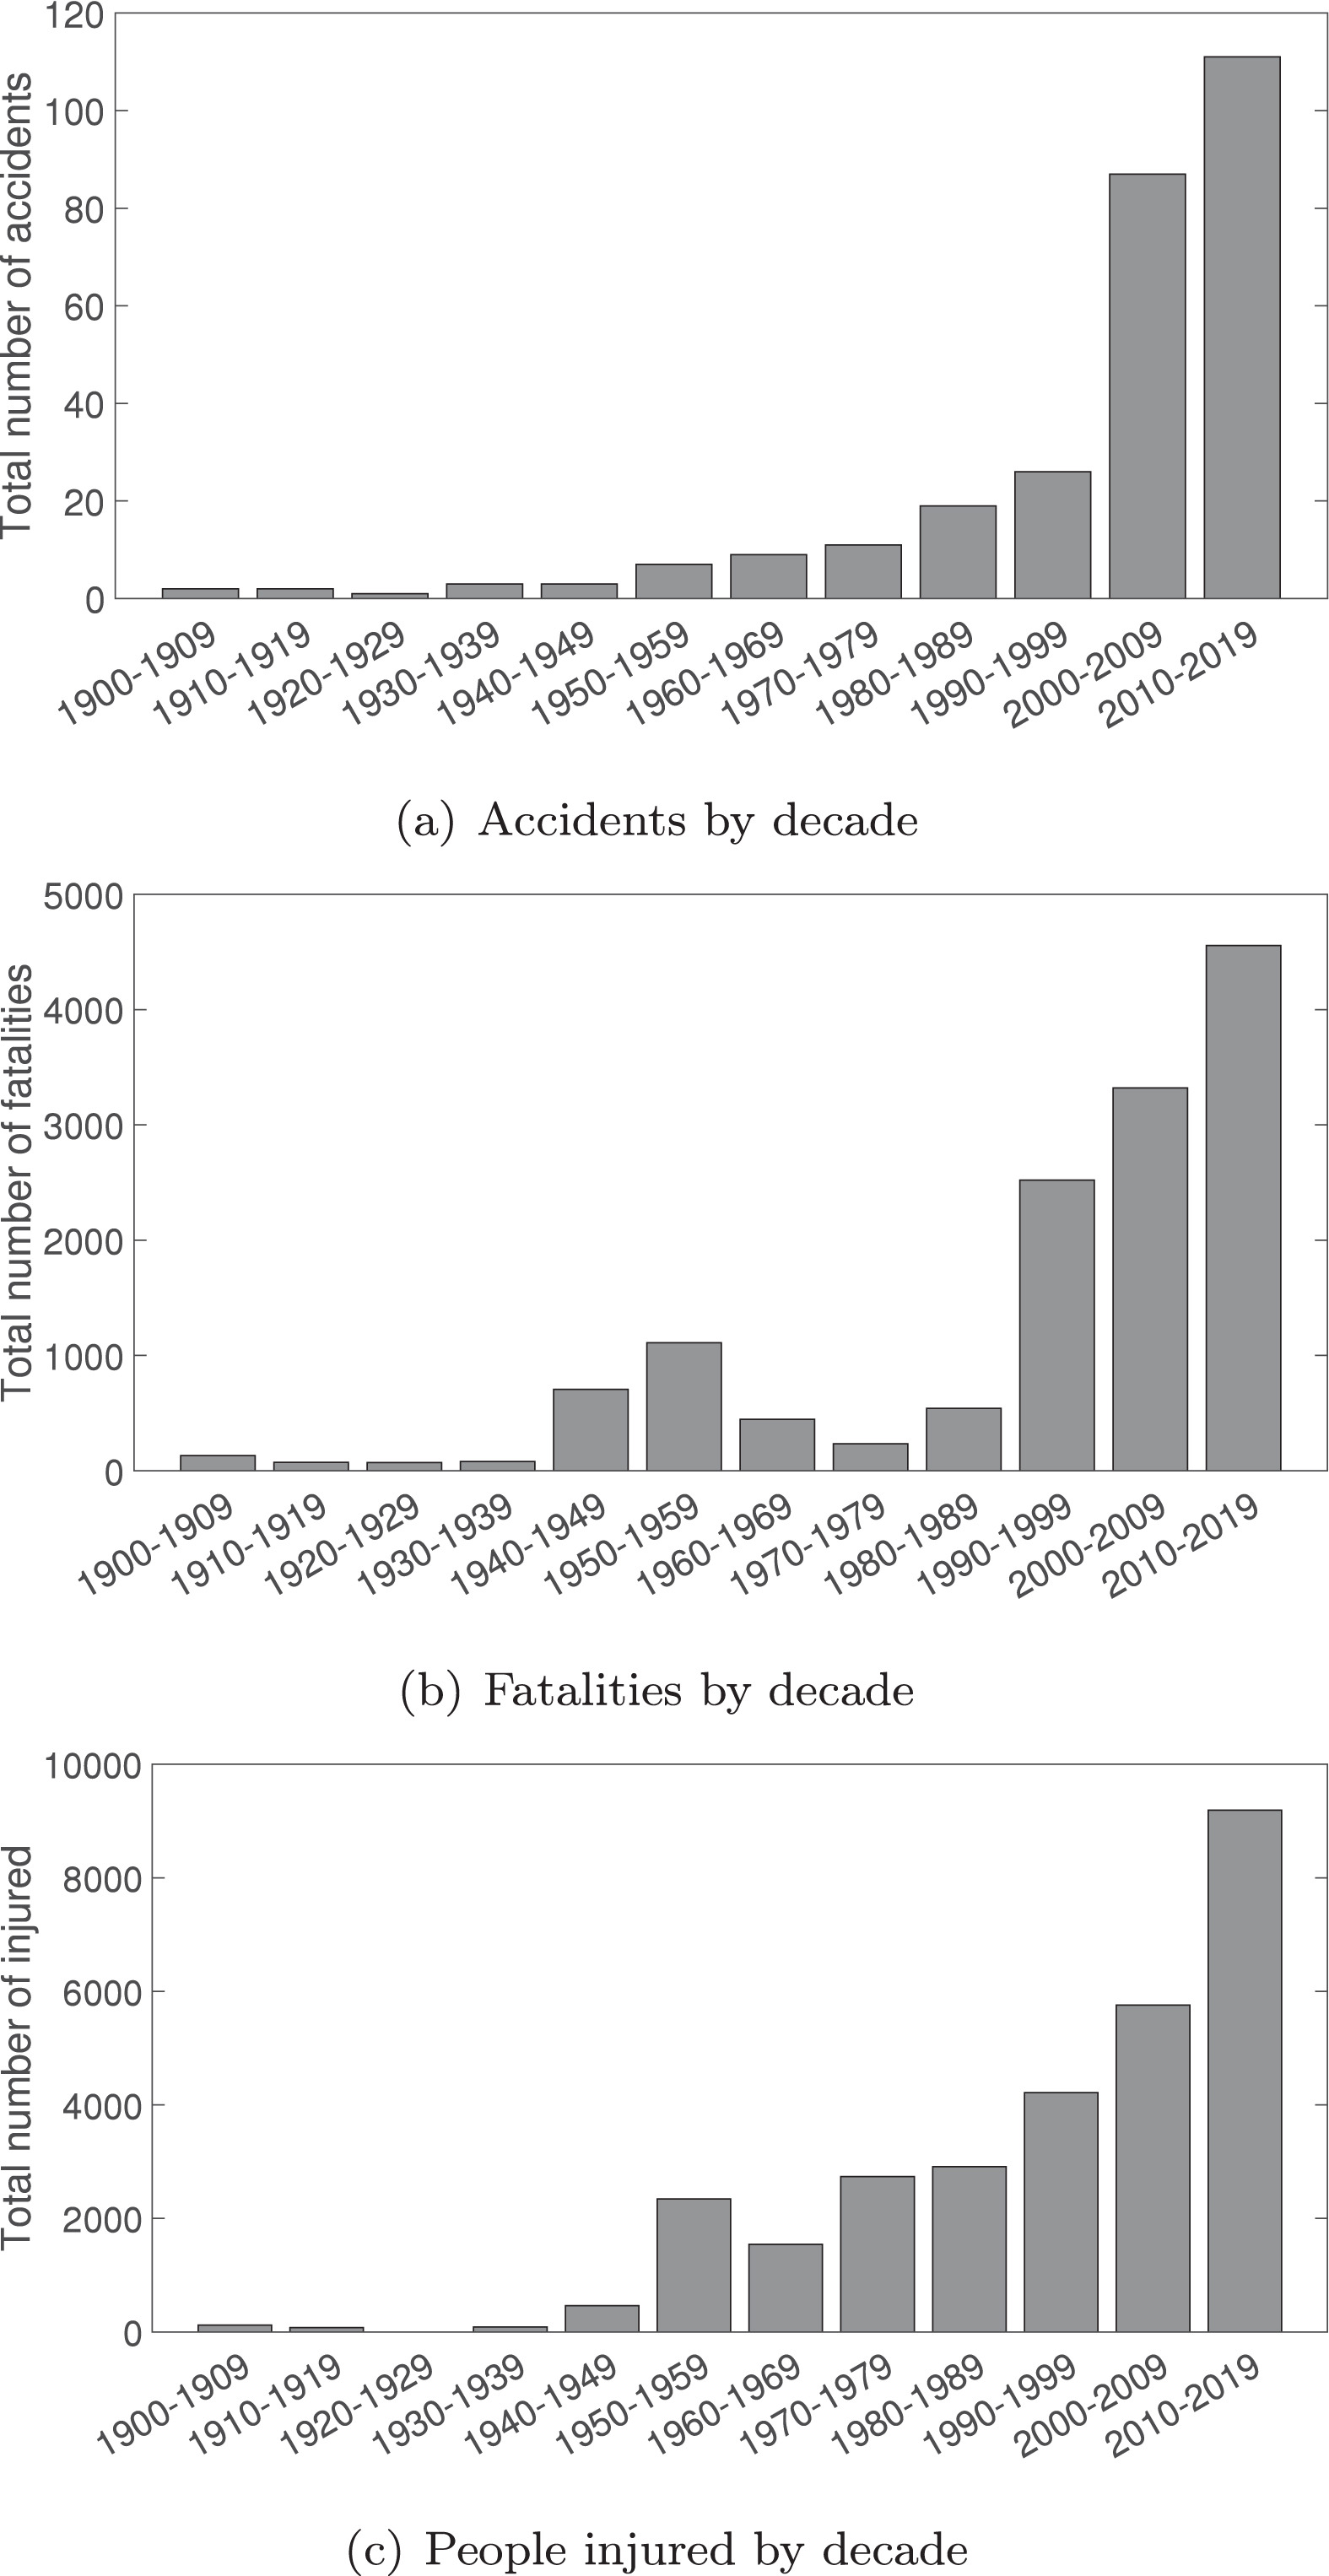
\includegraphics{../images/fatalities.jpg}

}

\caption{\label{fig-fatalities}Fatalities in crowds graph (Figure from
\protect\hyperlink{ref-FELICIANI2023106174}{Feliciani et al. 2023})}

\end{figure}

As seen from Figure~\ref{fig-fatalities} accidents, fatalities and
injuries at festivals and concerts worldwide are on the rise, with just
below 5.000 worldwide deaths in the decade of 2010-2019. The increasing
trend can be attributed to several causes, according to Raineri
(\protect\hyperlink{ref-inproceedings}{2004}): First of all, an increase
in the popularity of outdoor music festivals resulting in more and
larger festivals with large crowds. Also, high-risk behavior among crowd
attendants and the performing artist's music, behavior, and stage show
affects the crowd's safety. Cultural influence has also played a large
part in the safety of outdoor musical events. This can be behavior such
as crowd surfing, moshing, stage diving and the like.

It is worth mentioning that these figures and descriptions of situations
are often from media outlets. As such, it is not the full story. While
these statistics might make it seem that general safety and incidents at
festivals and the like have gotten worse, it is the opposite. It is
generally incredibly safe to attend these events, but using new
technologies we will attempt to enhance safety and comfort further.

At the same time, festivals in Denmark and the rest of the world have
had a focus on mitigating the safety risk in large crowds. This can be
seen by the establishment of the
\href{https://eventsafety.dk/historie}{Event Safety Foundation} in 2015.
This is a joint venture between the Skanderborg Festival Group
(Smukfest) and Muskelsvindfonden (Grøn Koncert). This foundation has the
purpose of securing the safety of the crowds at these two large Danish
festivals, as well as many other events in Denmark. They do this through
knowledge sharing, professionals and trained volunteers, courses and
counseling. This is the company that this project will be done in
collaboration with.

To have the best possible outcome for this project, Event Safety invited
us to Grøn Koncert and Smukfest in July and August to see how they work
and gather security video footage of real crowds at festivals to use as
training data. We will also use Event Safety for their practical and
theoretical knowledge of crowd safety to use in the system, user
feedback and user testing.

\hypertarget{sec-problem-statement}{%
\subsection{Problem Statement}\label{sec-problem-statement}}

Can computer vision software and AI techniques be leveraged to improve
crowd overview for security guards, by receiving video feed from large
crowds, and ultimately improve crowd safety?

\hypertarget{planning-and-method}{%
\subsection{Planning and method}\label{planning-and-method}}

In the context of developing a software system for our final project,
the Waterfall method is adopted as the project management approach. This
decision is informed by the specific requirements of the project,
including the size of the development group and the constrained
timeframe. The Waterfall model, characterised by its linear, sequential
and plan-driven approach, offers a structured framework that aligns well
with the project's objectives and constraints.

The Waterfall model follows the following approach
(\protect\hyperlink{ref-sommerville2011software}{Sommerville 2011}):

\begin{enumerate}
\def\labelenumi{\arabic{enumi}.}
\item
  Requirement analysis and definition.
\item
  System and software design.
\item
  Implementation and unit testing.
\item
  Integration and system testing.
\item
  Operation and maintenance: Not part of the scope. The project does,
  however, deliver documentation and user guides for future use.
\end{enumerate}

This project will largely follow this approach. There are however some
exceptions, including the types of tests performed in the implementation
and integration phases and the absence of the operation and maintenance
phase. These phases would be necessary for the use of our product after
the project but are not part of our project scope.

The Waterfall method was chosen for its clear, manageable workflow
suitable for a small two-member team compared to an agile Scrum
approach, its alignment with the project's timeline for delivering a
complex computer vision system, and its structured phases that ensure
thorough analysis, design, implementation, and testing.

The project timeline is structured into phases, each aligning with the
traditional stages of the Waterfall model as described above by
Sommerville (\protect\hyperlink{ref-sommerville2011software}{2011}). A
description of the planning of the project timeline can be seen here as
well as in Section~\ref{sec-appendices}. The following also includes a
description of the deliverables that are part of Sommerville's theory
behind the Waterfall method. These will be toned down to reduce the
documentation load and make up for the small group size.

\begin{enumerate}
\def\labelenumi{\arabic{enumi}.}
\item
  Preparation Phase (Pre-September): In this initial phase, the
  groundwork for the project is laid. This includes finalising the
  project description, establishing company collaborations, and
  collecting the necessary data. This phase is critical for ensuring
  that the project starts with a clear direction and the resources
  required for success.
\item
  Analysis and Design (September): The focus in September will be on
  analysing the collected data and designing the computer vision system.
  This stage involves understanding the requirements for crowd safety
  management and translating these into a viable software design. This
  phase delivers a requirement specification for the analysis and a
  software architecture design diagram for the design phase.
\item
  Implementation (October and November): During these months, the actual
  development of the software takes place. This phase involves coding
  the designed system, and ensuring that the software components are
  implemented correctly to achieve the desired functionality. This phase
  delivers an implemented system.
\item
  Testing (Early December): At the beginning of December, the system
  will undergo testing. This phase is crucial for identifying and
  rectifying any flaws or inefficiencies in the software. The testing
  phase ensures that the final product is reliable and meets the
  project's standards. This phase delivers a documented user test
  review.
\item
  Documentation and Reporting: Parallel to the other phases, the project
  report will be written continuously. This documentation will capture
  the development process, challenges, solutions, and overall learning
  from the project. The continuous nature of this task ensures that all
  aspects of the project are accurately and comprehensively recorded.
\end{enumerate}

Adopting the Waterfall method in this project provides a systematic and
predictable framework, crucial for managing the task of integrating
computer vision into crowd safety management and being able to deliver a
finished proof-of-concept. The structured phases of the Waterfall model
align well with the project's timelines and resource allocation,
ensuring a cohesive and efficient approach to achieving the project's
objectives.

\hypertarget{stakeholders}{%
\subsection{Stakeholders}\label{stakeholders}}

``Event Safety A/S'' is a key stakeholder in the project. The company,
its employees and its volunteers specialise in crowd safety management
at large-scale events like festivals, concerts, sporting events and
more. Their collaboration includes sharing expertise in crowd safety,
assisting in data collection through festival access, and offering
feedback for user testing. Event Safety will also provide theoretical
and practical insight into crowd safety and invite us to courses where
we can learn. Event Safety has an interest in the project's outcome, as
it directly aligns with their objective of improving event safety and
using new technology to fulfill this need better. The project team is
committed to fulfilling the project to Event Safety's needs by
integrating their insights, adhering to the responsible use of the data
collected on their festivals and ensuring the software system is
properly aligned with their interests, practically applicable and
effective in actual event scenarios.

\newpage{}

\hypertarget{sec-softa}{%
\section{State-of-the-art}\label{sec-softa}}

This section will describe the state-of-the-art technologies from
academic literature regarding computer vision and crowd counting that
will be used in this project.

\hypertarget{convolutional-neural-network-cnn-for-computer-vision}{%
\subsection{Convolutional Neural Network (CNN) for Computer
Vision}\label{convolutional-neural-network-cnn-for-computer-vision}}

Convolutional Neural Networks (CNN) are a type of Artificial Neural
Network (ANN) that are used to ``solve difficult image-driven pattern
recognition tasks.''
(\protect\hyperlink{ref-DBLP:journalsux2fcorrux2fOSheaN15}{O'Shea and
Nash 2015}) ANN's use input in the form of a multi-dimensional vector,
which will be distributed to several hidden layers. The hidden layers
will be weighted by evaluating how a stochastic change within itself
affects the final output (backpropagation). Deep learning is an ANN with
multiple hidden layers. ANN's can be either supervised: Being trained on
a set of labeled training data, or unsupervised: Having no labeled
training data, but instead minimising the result of the cost function.
According to O'Shea and Nash
(\protect\hyperlink{ref-DBLP:journalsux2fcorrux2fOSheaN15}{2015}) and
Lempitsky and Zisserman
(\protect\hyperlink{ref-NIPS2010_fe73f687}{2010}), supervised learning
is usually necessary for image-focused pattern recognition tasks.

CNNs are similar to ANNs in almost every way, with the only difference
being that CNNs allow encoding image-specific features such as edges,
textures, color patterns and shape features. This reduces the complexity
of a traditional ANN trained on image data, where a vector
representation grows in size exponentially depending on the image size.
Reducing the feature vector also reduces the risk of overfitting the
model. This is done through the process of convolution. In the
convolution layer, local regions of the image vector are scanned for
image-relevant features. Usually, the features are run through a pooling
layer, reducing its computational complexity by sampling and
down-scaling the features. This feature map is then fed to a traditional
ANN, with a given amount of hidden layers.

\hypertarget{solving-scale-variation-with-sasnet}{%
\subsection{Solving Scale-Variation with
SASNet}\label{solving-scale-variation-with-sasnet}}

Scale variation is one of the main challenges with crowd counting since
the perspective in the image will lead to different sizes of heads. One
solution to this is proposed by Song et al.
(\protect\hyperlink{ref-sasnet}{2021}). SASNet relies on the fact that
heads in a local path share roughly the same scale. It is currently not
a common approach to solve scale variation on a continuous scale. SASNet
solves it in 5 discrete steps using a weighted average. This bridges the
gap between discrete feature extraction and continuous feature
extraction. This architecture can be seen in Figure~\ref{fig-sasnet}.

\begin{figure}

{\centering 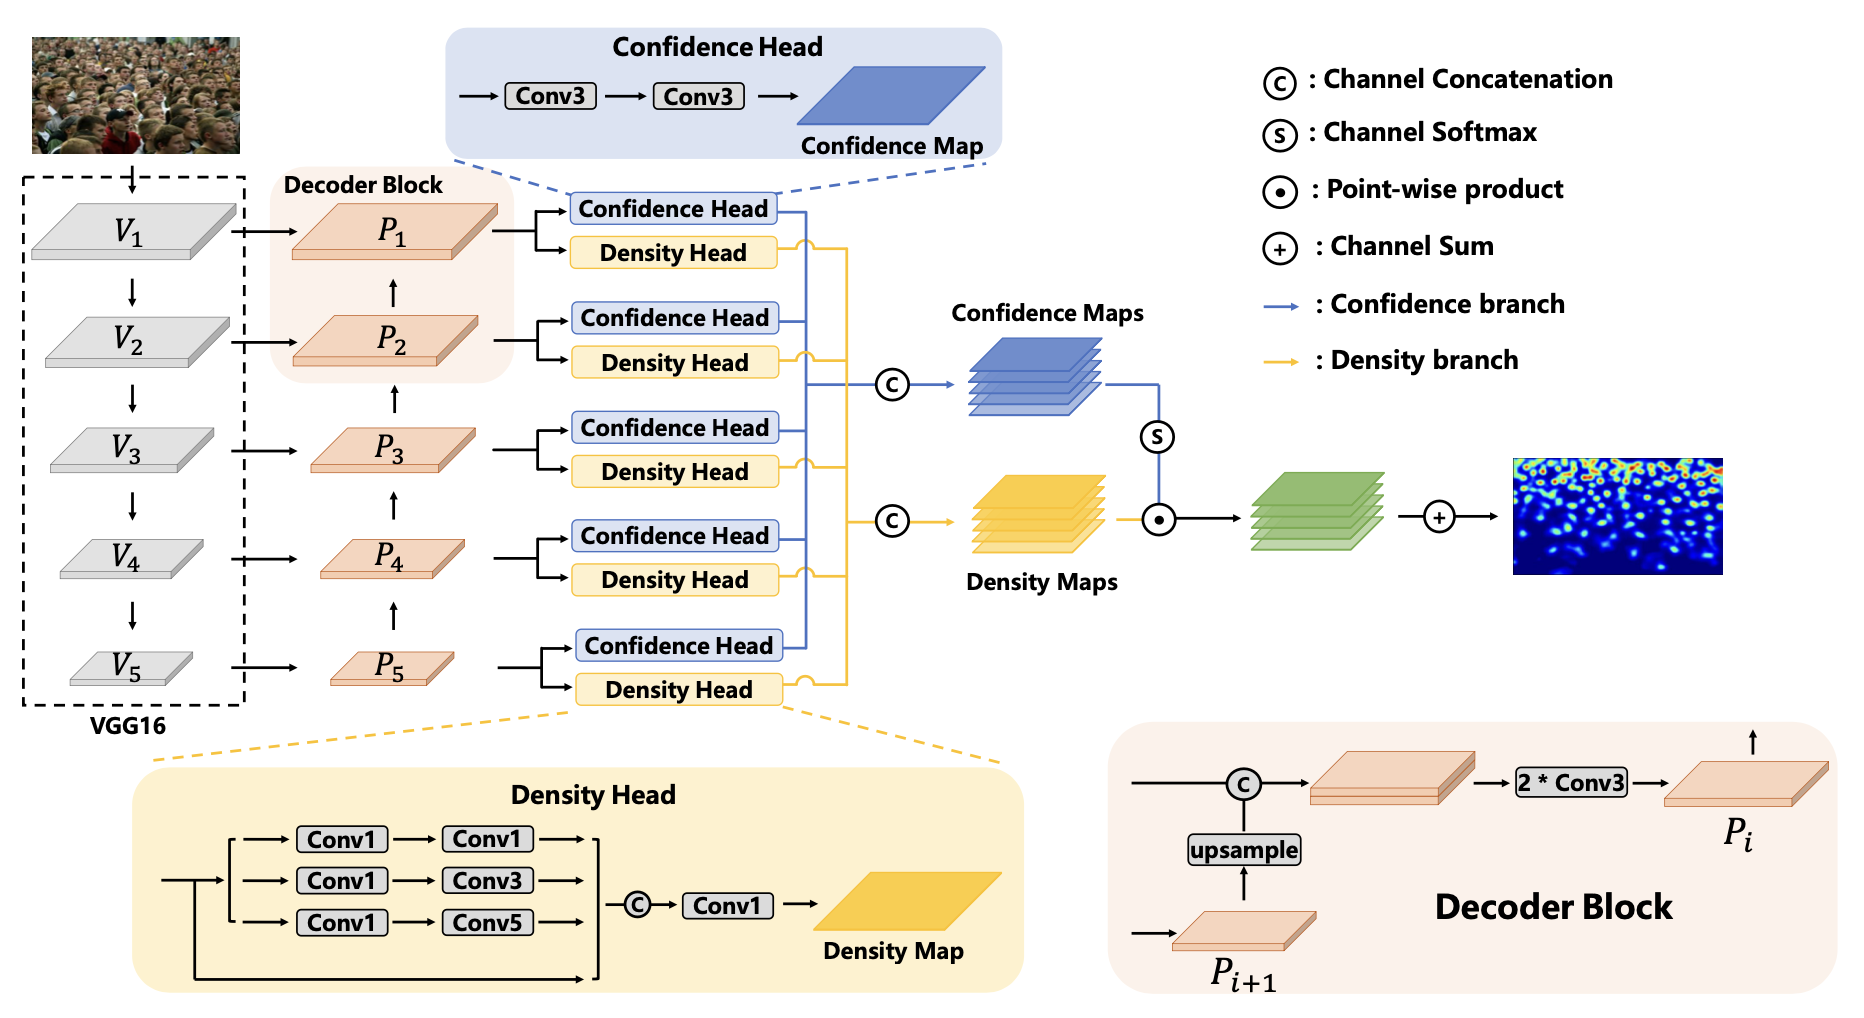
\includegraphics{../images/sasnet-architechture.png}

}

\caption{\label{fig-sasnet}Architecture of the SASNet model (Diagram
from \protect\hyperlink{ref-sasnet}{Song et al. 2021})}

\end{figure}

As can be seen from the diagram, SASNet uses the first 13 convolutional
layers from VGG-16 (\protect\hyperlink{ref-simonyan2014very}{Simonyan
and Zisserman 2014}) in the encoder. SASNet then produces 5 feature
levels with 5 levels of downsampling (\(V_n\)). It produces 5 levels of
predictions (\(P_n\)). This is what is referred to as the ``U-shaped
backbone''. These are then fed to a confidence branch and a density
branch that produces a confidence map and density map for each of the 5
levels. The complete density map is a product of the sum of the
individual density and confidence branches using a softmax function for
the confidence.

\hypertarget{leading-practical-projects-of-the-state-of-the-art-crowd-management-systems}{%
\subsection{Leading practical projects of the state-of-the-art crowd
management
systems}\label{leading-practical-projects-of-the-state-of-the-art-crowd-management-systems}}

While there are some academic research projects on crowd counting, the
practical implementations of this technology are hard to find. In
practice, the leading method of crowd counting is a variation of using
turnstiles and expertise in knowing what certain densities of people
look like and multiplying it with the area of the space, also known as
Jacob's method. (\protect\hyperlink{ref-dahl2023crowd}{Dahl 2023})
(\protect\hyperlink{ref-Still2014CrowdScience}{Still 2014}) Fruin's
Level of Service (LOS) is then applied to these densities. The LOS
standard is a measure of how many square meters each person needs to
feel comfortable when walking, climbing stairs or standing/queuing. The
LOS standard is based on a series of qualitative and quantitative
methods (\protect\hyperlink{ref-fruin1971pedestrian}{Fruin 1971}).
Fruin's LOS can be seen in Table~\ref{tbl-los}.

\hypertarget{tbl-los}{}
\begin{longtable}[]{@{}ll@{}}
\toprule\noalign{}
LOS & Density \\
\midrule\noalign{}
\endfirsthead
\toprule\noalign{}
LOS & Density \\
\midrule\noalign{}
\endhead
\bottomrule\noalign{}
\endlastfoot
LOS A & \textless{} 0.83 people per sq. meter \\
& \\
LOS B & \textless{} 1.07 people per sq. meter \\
& \\
LOS C & \textless{} 1.54 people per sq. meter \\
& \\
LOS D & \textless{} 3.58 people per sq. meter \\
& \\
LOS E & \textless{} 5.38 people per sq. meter \\
& \\
LOS F & \textgreater{} 5.38 people per sq. meter \\
\caption{\label{tbl-los}Table of Fruin's Level of Service (LOS). By
Fruin (\protect\hyperlink{ref-fruin1971pedestrian}{1971}). Originally in
square feet per person. Converted to densities (people per square meter)
with the formula
\(density=(1/feet per person)*10.763915\)}\tabularnewline
\end{longtable}

Depending on the type of festival Event Safety works with different
acceptable LOS. At Grøn which is a more family-friendly festival with
people sitting an acceptable service level might be LOS D close to the
stage and LOS C farther from the stage. At Smukfest an acceptable LOS
might be LOS D or near LOS E in some places. LOS F is usually never
acceptable as this can quickly become a safety issue.
(\protect\hyperlink{ref-dahl2023crowd}{Dahl 2023})

According to the best of our collaborators at Event Safety's knowledge,
there have not been any real projects that aim to use technology for
crowd counting and density estimations at festivals and concerts in
Denmark, nor any large-scale projects in Europe. The only example they
know of was a project at Roskilde Festival that tried to use cell data
to generate a heatmap of crowd densities and crowd size. This project
was abandoned because of its inaccuracy.

Commercial applications for object-detection-based cameras are
implemented at some places like airports, malls, sidewalks and
supermarkets to manage queues, flow and count small numbers of people.
This is products like
\href{https://www.hikvision.com/en/solutions/solutions-by-function/people-counting/}{Hikvision},
\href{https://www.terabee.com/products/people-counting/}{TeraBee},
\href{https://haltian.com/products/people-counting/}{Haltian},
\href{https://www.footfallcam.com/}{FootfallCam}. We have not been able
to find projects that use cameras to create a detailed heatmap of
densities and total crowd counts in a large area, with high density and
using existing surveillance camera infrastructure that does not
necessarily have to be high resolution.

\hypertarget{related-technologies}{%
\subsection{Related technologies}\label{related-technologies}}

A more advanced and evolved form of crowd counting is known as crowd
localisation. Gao, Gong, and Li
(\protect\hyperlink{ref-DBLP:journalsux2fcorrux2fabs-2108-00584}{2021})
Crowd localisation provides more in-depth data for each instance in the
crowd, meaning the position (and relative position) of individuals or
groups in a crowd. This is useful for analysing flow estimation or more
precise crowd counting. Crowd localisation is still a highly discussed
and continuously researched topic. For these reasons, we found
crowd-counting technologies more relevant to our project.

\newpage{}

\hypertarget{sec-analysis}{%
\section{Analysis}\label{sec-analysis}}

This section will describe the analysis of the problem statement and
define the outline of the system and functional- and non-functional
system requirements.

\hypertarget{system-specification}{%
\subsection{System specification}\label{system-specification}}

Using cameras mounted around a hotspot of a crowd or on a stationary
drone, we aim to develop a platform where an AI model receives video
footage from these cameras, uses the model to count the crowd, and helps
safety experts recognise a dangerous situation. This could be one or
more of the following (\protect\hyperlink{ref-inproceedings}{Raineri
2004}):

\begin{itemize}
\tightlist
\item
  Several people moving into the crowd from a specific direction create
  a dangerous pressure point
\item
  More than a specified amount of people in a marked area resulting in
  unsafe conditions (ie. \textgreater6 people per square meter)
\item
  Omnidirectional or directional movement in the crowd resulting in a
  dangerous situation
\item
  An area in the crowd suddenly being void of people, perhaps hinting at
  a mosh pit or an emergency
\end{itemize}

These are some of the situations this project aims to systematically
detect and alert professionals by providing meaningful feedback.

The system would consist of the following:

\begin{enumerate}
\def\labelenumi{\arabic{enumi}.}
\tightlist
\item
  A backend that receives the data from the cameras, with an
  implementation of a CNN to handle the video feed according to the
  bullet list above and exposes this data through an API.
\item
  A frontend or GUI to display this information in a meaningful way.
  This could be through a heat map, a numerical estimate of a risk
  factor, or other visual output.
\end{enumerate}

\begin{figure}

{\centering 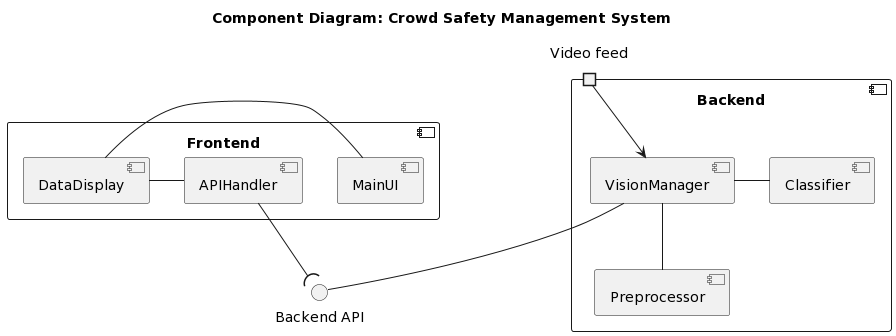
\includegraphics[width=\textwidth,height=0.5\textheight]{../images/component-diagram-1.png}

}

\caption{\label{fig-component-diagram}Component diagram of the system}

\end{figure}

An initial component diagram that maps this described system but is
subject to change can be seen in Figure~\ref{fig-component-diagram}.

\hypertarget{sec-functional-requirements}{%
\subsection{Functional Requirements}\label{sec-functional-requirements}}

This section describes the functional requirements for the proposed
system along with their ``MoSCoW'' prioritisation (``must have'',
``should have'', ``could have'', and ``will not have''). These are shown
in Table~\ref{tbl-functional-reqs}.

\hypertarget{tbl-functional-reqs}{}
\begin{longtable}[]{@{}
  >{\raggedright\arraybackslash}p{(\columnwidth - 4\tabcolsep) * \real{0.0429}}
  >{\raggedright\arraybackslash}p{(\columnwidth - 4\tabcolsep) * \real{0.2000}}
  >{\raggedright\arraybackslash}p{(\columnwidth - 4\tabcolsep) * \real{0.7571}}@{}}
\toprule\noalign{}
\begin{minipage}[b]{\linewidth}\raggedright
\textbf{ID}
\end{minipage} & \begin{minipage}[b]{\linewidth}\raggedright
\textbf{MoSCoW}
\end{minipage} & \begin{minipage}[b]{\linewidth}\raggedright
\textbf{Requirement}
\end{minipage} \\
\midrule\noalign{}
\endfirsthead
\toprule\noalign{}
\begin{minipage}[b]{\linewidth}\raggedright
\textbf{ID}
\end{minipage} & \begin{minipage}[b]{\linewidth}\raggedright
\textbf{MoSCoW}
\end{minipage} & \begin{minipage}[b]{\linewidth}\raggedright
\textbf{Requirement}
\end{minipage} \\
\midrule\noalign{}
\endhead
\bottomrule\noalign{}
\endlastfoot
1 & M & The system \textbf{must} be able to count the number of people
in the crowd with the accuracy required by the user base \\
& & \\
2 & M & The system \textbf{must} be able to segment the crowd into
virtual sections for further processing \\
& & \\
3 & M & The system \textbf{must} be able to create a heatmap of the
crowd density \\
& & \\
4 & S & The system \textbf{should} be able to calculate the physical
density of humans per square meter \\
& & \\
5 & S & The system \textbf{should} be able to detect the movement of
crowd sections \\
& & \\
6 & S & The system \textbf{should} be able to correct for camera
distortion, warp and perspective \\
& & \\
7 & S & The system \textbf{should} be able to detect choke points in the
crowd movements \\
& & \\
8 & S & The system \textbf{should} be able to generate a summarising
report of the concert with statistics of relevant safety indicators
(crowd density, crowd count, risk factors, choke points, and others)
after the event \\
& & \\
9 & C & The system \textbf{could} be able to estimate a numerical risk
factor based on available factors \\
& & \\
10 & C & The system \textbf{could} be able to generate a live, or
delayed, video overlaid user interface \\
& & \\
11 & W & The system \textbf{will not} be able to identify dangerous
situations that might call for cautionary actions such as crowd surges,
mosh pits, falls, blocked exits, etc. \\
& & \\
12 & W & The system \textbf{will not} be able to use data gathered
elsewhere at a concert such as alcohol sales, average crowd age, sound,
artists, etc. to give a more precise crowd profile and thus risk
factor \\
\caption{\label{tbl-functional-reqs}Table of functional
requirements}\tabularnewline
\end{longtable}

\hypertarget{sec-non-functional-requirements}{%
\subsection{Non-functional
requirements}\label{sec-non-functional-requirements}}

This section describes the non-functional requirements for the proposed
system along with their ``MoSCoW'' prioritisation (``must have'',
``should have'', ``could have'', ``will not have''). These are shown in
table Table~\ref{tbl-nonfunctional-reqs}.

\hypertarget{tbl-nonfunctional-reqs}{}
\begin{longtable}[]{@{}
  >{\raggedright\arraybackslash}p{(\columnwidth - 4\tabcolsep) * \real{0.0429}}
  >{\raggedright\arraybackslash}p{(\columnwidth - 4\tabcolsep) * \real{0.2000}}
  >{\raggedright\arraybackslash}p{(\columnwidth - 4\tabcolsep) * \real{0.7571}}@{}}
\toprule\noalign{}
\begin{minipage}[b]{\linewidth}\raggedright
\textbf{ID}
\end{minipage} & \begin{minipage}[b]{\linewidth}\raggedright
\textbf{MoSCoW}
\end{minipage} & \begin{minipage}[b]{\linewidth}\raggedright
\textbf{Requirement}
\end{minipage} \\
\midrule\noalign{}
\endfirsthead
\toprule\noalign{}
\begin{minipage}[b]{\linewidth}\raggedright
\textbf{ID}
\end{minipage} & \begin{minipage}[b]{\linewidth}\raggedright
\textbf{MoSCoW}
\end{minipage} & \begin{minipage}[b]{\linewidth}\raggedright
\textbf{Requirement}
\end{minipage} \\
\midrule\noalign{}
\endhead
\bottomrule\noalign{}
\endlastfoot
1 & M & The system \textbf{must} protect the privacy of the personal
data \\
& & \\
2 & S & The system \textbf{should} have a user-friendly interface that
is easy to manage for both technical and non-technical users \\
& & \\
3 & S & The system \textbf{should} have adequate documentation /
technical specification for technical users \\
& & \\
4 & S & The system \textbf{should} have adequate user manuals for
non-technical users \\
& & \\
5 & C & The system \textbf{could} have high reliability that is not
based on the visual circumstances and environment (e.g.~sunlight, stage
light, audience flashlights, and other visual effects) or report
confidence based on environment \\
& & \\
6 & C & The system \textbf{could} be scalable to simultaneous
interoperability between multiple cameras \\
& & \\
7 & C & The system \textbf{could} integrate with existing CCTV software
systems at venues \\
\caption{\label{tbl-nonfunctional-reqs}Table of non-functional
requirements}\tabularnewline
\end{longtable}

\hypertarget{sec-risks}{%
\subsection{Risk analysis}\label{sec-risks}}

More often than not a project will encounter problems that can hinder
the progress or outcome. By being well prepared we are able to mitigate
some of these risks. Table~\ref{tbl-risks} describes some of the risks
we might encounter in this project.

\hypertarget{tbl-risks}{}
\begin{longtable}[]{@{}
  >{\raggedright\arraybackslash}p{(\columnwidth - 8\tabcolsep) * \real{0.2000}}
  >{\raggedright\arraybackslash}p{(\columnwidth - 8\tabcolsep) * \real{0.2000}}
  >{\raggedright\arraybackslash}p{(\columnwidth - 8\tabcolsep) * \real{0.2000}}
  >{\raggedright\arraybackslash}p{(\columnwidth - 8\tabcolsep) * \real{0.2000}}
  >{\raggedright\arraybackslash}p{(\columnwidth - 8\tabcolsep) * \real{0.2000}}@{}}
\toprule\noalign{}
\begin{minipage}[b]{\linewidth}\raggedright
\textbf{ID}
\end{minipage} & \begin{minipage}[b]{\linewidth}\raggedright
\textbf{Name}
\end{minipage} & \begin{minipage}[b]{\linewidth}\raggedright
\textbf{Affects}
\end{minipage} & \begin{minipage}[b]{\linewidth}\raggedright
\textbf{Description}
\end{minipage} & \begin{minipage}[b]{\linewidth}\raggedright
\textbf{Mitigation}
\end{minipage} \\
\midrule\noalign{}
\endfirsthead
\toprule\noalign{}
\begin{minipage}[b]{\linewidth}\raggedright
\textbf{ID}
\end{minipage} & \begin{minipage}[b]{\linewidth}\raggedright
\textbf{Name}
\end{minipage} & \begin{minipage}[b]{\linewidth}\raggedright
\textbf{Affects}
\end{minipage} & \begin{minipage}[b]{\linewidth}\raggedright
\textbf{Description}
\end{minipage} & \begin{minipage}[b]{\linewidth}\raggedright
\textbf{Mitigation}
\end{minipage} \\
\midrule\noalign{}
\endhead
\bottomrule\noalign{}
\endlastfoot
R01 & Code is lost & Project, product & If the code is lost or corrupted
& Having a version control system for the codebase and report. \\
& & & & \\
R02 & Technology constraints & Product & If the used or available
technology is inadequate for the remaining requirements defined in the
project & Find alternative technologies or solutions for our
requirements before a barrier might be reached. Research the technology
and options in depth before implementation. Discuss with our supervisor
if alternatives exist. \\
& & & & \\
R03 & Personal Conflicts & Product, project & A project-related or
personal conflict between the 2 members of the project affecting either
the further development or the project as a whole. & Keeping a friendly
and open mindset in the work will take us far. Depending on the nature
of a potential conflict we would either discuss and solve it outside of
work or discuss it with our supervisor. \\
& & & & \\
R04 & Unusable data & Project, Product & If the data provided by the
drone or from Event Safety turns out to be unusable due to one or more
factors: Resolution, perspective, distortion etc. & Making sure that
provided data is on par regarding the requirements of our project. Some
data might be fixed by using mathematical algorithms but in general, a
proper standard for data is preferred. Can be replaced by data found
online, but will not have the same effect. \\
& & & & \\
R05 & Company collaboration ends & Project & If Event Safety or the
group decides to end the collaboration around the project early. &
Making sure that we listen to and adapt to feedback from Event Safety to
keep our good relationship with them. \\
\caption{\label{tbl-risks}Table of risks and their
impact}\tabularnewline
\end{longtable}

\hypertarget{sec-riskass}{%
\subsection{Risk assessment}\label{sec-riskass}}

To fully assess the risks described above it is vital that the
probability and severity of each risk is assessed. This is done by using
the following formula:

\[
Effect = Probabilty * Severity
\]

The probability and severity are given each given a score between 1 and
5. 1 being a low probability/severity and 5 being a very high
probability/severity. The effect is then calculated based on these
numbers. This can be seen in Table~\ref{tbl-risk-assesment}.

\hypertarget{tbl-risk-assesment}{}
\begin{longtable}[]{@{}
  >{\raggedright\arraybackslash}p{(\columnwidth - 8\tabcolsep) * \real{0.2000}}
  >{\raggedright\arraybackslash}p{(\columnwidth - 8\tabcolsep) * \real{0.2000}}
  >{\raggedright\arraybackslash}p{(\columnwidth - 8\tabcolsep) * \real{0.2000}}
  >{\raggedright\arraybackslash}p{(\columnwidth - 8\tabcolsep) * \real{0.2000}}
  >{\raggedright\arraybackslash}p{(\columnwidth - 8\tabcolsep) * \real{0.2000}}@{}}
\toprule\noalign{}
\begin{minipage}[b]{\linewidth}\raggedright
\textbf{ID}
\end{minipage} & \begin{minipage}[b]{\linewidth}\raggedright
\textbf{Probablity}
\end{minipage} & \begin{minipage}[b]{\linewidth}\raggedright
\textbf{Severity}
\end{minipage} & \begin{minipage}[b]{\linewidth}\raggedright
\textbf{Effect}
\end{minipage} & \begin{minipage}[b]{\linewidth}\raggedright
\textbf{Notes}
\end{minipage} \\
\midrule\noalign{}
\endfirsthead
\toprule\noalign{}
\begin{minipage}[b]{\linewidth}\raggedright
\textbf{ID}
\end{minipage} & \begin{minipage}[b]{\linewidth}\raggedright
\textbf{Probablity}
\end{minipage} & \begin{minipage}[b]{\linewidth}\raggedright
\textbf{Severity}
\end{minipage} & \begin{minipage}[b]{\linewidth}\raggedright
\textbf{Effect}
\end{minipage} & \begin{minipage}[b]{\linewidth}\raggedright
\textbf{Notes}
\end{minipage} \\
\midrule\noalign{}
\endhead
\bottomrule\noalign{}
\endlastfoot
R01 & 1 & 3 & 3 & The severity is based on the amount of code lost. \\
& & & & \\
R02 & 2 & 2 & 4 & Compute power limitations are the primary factor here.
However, we do not see the need for more than what accessible computing
resources can provide. \\
& & & & \\
R03 & 1 & 1 & 1 & Given the nature of previous work in semester projects
and friendship this is highly unlikely. \\
& & & & \\
R04 & 4 & 2 & 8 & The severity depends on how bad the data is and how
well we are able to adapt to it. \\
& & & & \\
R05 & 1 & 5 & 5 & Severity would depend on when in the process Event
Safety would cancel our collaboration. \\
\caption{\label{tbl-risk-assesment}Table of risk
assessment}\tabularnewline
\end{longtable}

Based on the table above, we can deduce that the major risk we should be
aware of is R04. How we handle the possibility of unusable data is
crucial to the success of this project. While other risks also have high
effects, their probability is too low to be considered threatening to
the project. However, having measurements in place to counteract every
risk is still important.

\newpage{}

\hypertarget{sec-design}{%
\section{Design}\label{sec-design}}

This chapter is going to describe the design choices made for the system
as a whole regarding the analysis of the problem in general and
requirement specification. This chapter will talk about approaches to
crowd counting and how crowd counting differs from object detection.
Following this, the chapter talks about the selection process for a
cloud computing service and why we decided to go with SASNet as the
model for this project

\hypertarget{sec-design-crowdcounting}{%
\subsection{About the choice of crowd
counting}\label{sec-design-crowdcounting}}

Crowd counting is a field of computer vision research that has developed
quickly in recent years. It is a technique that aims to count the
instances of any object in an image, no matter the context or density.
(\protect\hyperlink{ref-sasnet}{Song et al. 2021})

One of the original ideas for solving this problem was to use Meta's SAM
model. During the preliminary research sessions, it was discovered that
SAM was not adequate in counting people but better suited for object
detection. The following citation from Ma, Hong, and Shangguan
(\protect\hyperlink{ref-ma2023sam}{2023}) highlights the problems well:

``Although the Segment Anything model (SAM) has shown impressive
performance in many scenarios, it currently lags behind state-of-the-art
few-shot counting methods, especially for small and congested objects.
We believe that this is due to two main reasons. Firstly, SAM tends to
segment congested objects of the same category with a single mask.
Secondly, SAM is trained with masks that lack semantic class
annotations, which could hinder its ability to differentiate between
different objects. Nevertheless, further exploration of adapting SAM to
the object counting task is still worth studying.''
(\protect\hyperlink{ref-ma2023sam}{Ma, Hong, and Shangguan 2023})

SAM and other object detection methods (sometimes described as ``crowd
counting by detection'') are usually trained on one specific type of
object by extracting certain visual features. The benefits of using
crowd counting rather than object detection are:

\begin{itemize}
\item
  Crowd counting is less intensive on computing resources.
\item
  Crowd counting performs better in crowded scenes with varying scales
  of objects and overlapping objects.
\item
  Crowd counting is more robust in environments with changes in light,
  without the need for specific training data.
\item
  Crowd counting is not as exposed to the risk of overfitting the model.
  (\protect\hyperlink{ref-li2021approaches}{Li et al. 2021})
\item
  Crowd counting does not single out individuals, but looks at the crowd
  holistically. (\protect\hyperlink{ref-chan2008}{Chan, Liang, and
  Vasconcelos 2008})
\end{itemize}

For these reasons, crowd counting is a method that can be used for many
domains including traffic and parking analysis, pedestrian crowds, corn
and crop counting, and much more. This project will use crowd-counting
methods to analyse, count and estimate the density of concert crowds.

(\protect\hyperlink{ref-li2021approaches}{Li et al. 2021}) says the
current leading approach to crowd counting is the use of a
regression-based method, especially in large crowds where detection
might not suffice. This paper, contrary to our definition of crowd
counting, includes object detection as a method of crowd counting. The
main challenge with regression-based methods for crowd counting is to
differentiate between the large-scale variations in the countable human
heads. (\protect\hyperlink{ref-li2021approaches}{Li et al. 2021})
discusses several categories of approaches for regression-based models
to solve scale variation problems, one of which is multi-scale fusion.
This approach is the category that this paper proposes for further
research, as it shows promising results in the balance between
performance and accuracy.

For the reasons outlined here from O'Shea and Nash
(\protect\hyperlink{ref-DBLP:journalsux2fcorrux2fOSheaN15}{2015}) and Li
et al. (\protect\hyperlink{ref-li2021approaches}{2021}), this project
will focus on the use of CNN and regression-based models for crowd
counting.

One of the useful datasets for crowd counting, ``ShanghaiTech'' comes
from the paper Zhang et al.
(\protect\hyperlink{ref-Zhang_2016_CVPR}{2016}). In this paper, there
are defined two datasets, ``part a'' and ``part b''. For the CSMS data,
``ShanghaiTech Part A'' is a more representative dataset to use, since
it contains more densely populated crowds from a bird's eye view. The
dataset is labeled with one dot representing roughly the middle of a
person's head. This is the approach outlined in one of the founding
papers of crowd counting: Lempitsky and Zisserman
(\protect\hyperlink{ref-NIPS2010_fe73f687}{2010}). In Lempitsky and
Zisserman (\protect\hyperlink{ref-NIPS2010_fe73f687}{2010}), it is
explained how their approach to crowd counting, which has become the
primary method in the field, is to create a density function \(F\) as a
function of the pixels in an image \(I\). This density function is
analogous to the physical idea of density, however not a direct
representation of the same concept, as physical density is based on
physical area. Integrating \(F\) over the entire image \(I\) will return
the number of people in \(I\).
(\protect\hyperlink{ref-NIPS2010_fe73f687}{Lempitsky and Zisserman
2010}) Each object in the image I should be represented by a normalised
2D Gaussian kernel with the mean at the person's head.

One disadvantage of this approach is that the kernel for objects close
to the edge of the image will not be counted as a whole object when
summed. It is not assumed that this will pose a significant source of
error for the CSMS. The downside of using the crowd counting approach is
that it will be difficult to track the movement of members of the crowd,
rather than using a detection-based counting method. Regression-based
crowd counting might also perform worse for very small crowds as it
relies on overall patterns in crowds. Despite this, and because this can
be seen as an advantage from a privacy point of view (see
Section~\ref{sec-facial-recognition}), the choice was made together with
our collaborators to use the regression-based method.

\hypertarget{design-considerations-regarding-security-and-privacy}{%
\subsection{Design considerations regarding security and
privacy}\label{design-considerations-regarding-security-and-privacy}}

Being citizens of and using the data of people from an EU country, we
have to abide by the rules of GDPR. This means that security and privacy
around the data that we have acquired are crucial. Practically, this
means that we have a responsibility to make sure that we only upload the
images and videos we need to run the model on when they need to be there
and remove them when not needed. In a perfect world, we would run our
program locally to limit the uploading and removal of sensitive data. It
is of course also necessary to consider the business and ethical
considerations of how using CCTV and computer vision more extensively
can affect some peoples' sense of privacy when attending a festival.

\hypertarget{sec-facial-recognition}{%
\subsubsection{Facial recognition vs.~Crowd
Counting}\label{sec-facial-recognition}}

When reading through this project, one might assume that privacy around
facial recognition would be an issue. However, as this is related to
heatmaps, crowd counting and crowd density of people, not facial
recognition, the identity of people in our footage is not a major
concern and thus was not featured in our risk management section. The
CSMS anonymises the output data and does not track individuals through
time, which could be a privacy concern.\\

\hypertarget{selecting-a-cloud-computing-service}{%
\subsubsection{Selecting a cloud computing
service}\label{selecting-a-cloud-computing-service}}

Initially, the backend of this project was run on a paid but still
resource-limited version of Google Collab - a Jupyter Notebook
collaboration space with access to cloud computing CPU and GPUs.
However, it was decided to research possible alternatives for easier
scalability and maintainability. When talking about renting cloud
computing GPU, the main factor is cost, as with enough money you can
rent almost unlimited cloud processing power. However, for our project
the amount of processing power available was not the primary concern -
data security was. This brought our attention away from international
services like Google Cloud/vertex and Amazon AWS to a local service:
UCloud. UCloud is a capable cloud computing service hosted locally on
SDU. Through our supervisor, we took action and applied for resources
for this project which were quickly granted. This allowed us to move our
initial backend to UCloud, which was a major progression for the
following reasons:

\begin{enumerate}
\def\labelenumi{\arabic{enumi}.}
\item
  UCloud is ``free'' for students and approved projects. You apply for a
  set amount of currency to use on the platform.
\item
  UCloud processing power is only limited by the amount of currency
  available to us on the platform, unlike Google Collab which was
  limited based on current global usage.
\end{enumerate}

As mentioned, data handling and data privacy are very important for this
project. With this in mind, we decided to research the policies of
UCloud regarding data handling before implementing our software on the
platform. According to SDU Cloud
(\protect\hyperlink{ref-UCloud_Security}{2020}), UCloud is ISO 27001
certified. This means that the platform lives up to an international
standard for information security management systems
(\protect\hyperlink{ref-iso27001}{International Organization for
Standardization 2013}). Furthermore, according to SDU Cloud
(\protect\hyperlink{ref-UCloud_Security}{2020}), UCloud is hosted
locally on SDU and not by a 3rd party operator. Using this information,
we can conclude that UCloud as a platform is safe to use for our project
and regulated to relevant standards.

\hypertarget{sec-model-selection}{%
\subsection{Choosing a technology for Crowd
Counting}\label{sec-model-selection}}

There are many open-source implementations of crowd counting models,
many of which can be seen in the
\href{https://github.com/gjy3035/Awesome-Crowd-Counting}{Awesome Crowd
Counting} repository by Gong
(\protect\hyperlink{ref-gjy3035_awesome_crowd_counting}{2023}) along
with research papers and benchmarks. After careful consideration, the
choice of using SASNet was based on four different factors:

\begin{enumerate}
\def\labelenumi{\arabic{enumi}.}
\item
  SASNets fits our need to solve the problem of scale variation in the
  video material. It was not possible to obtain video material from an
  approximate orthographic perspective. However, future endeavors for
  this project might include cameras like those from one of our
  collaborators \href{https://www.phaseone.com/}{PhaseOne} who produces
  approximate orthographic perspectives using high pixel density cameras
  from high altitudes. SASNet, however, fulfills the requirement to
  produce relatively high accuracy prediction on an image with
  perspective for now.
\item
  SASNet has some of the lowest absolute errors on the ShanghaiTech
  testing data, according to Gong
  (\protect\hyperlink{ref-gjy3035_awesome_crowd_counting}{2023}) which
  compares at least 45 different crowd-counting models and methods.
\item
  SASNet is open source and licensed under the permissive Apache 2.0
  license, which allows us to use it legally and for free in our
  project. SASNet also publishes the pre-trained model weights (trained
  on ShanghaiTech A and B), which means we can save many computing- and
  time resources instead of training the model ourselves.
\item
  SASNet publishes the model weights from the training on either
  ShanghaiTech part A or part B. For this project, it is deemed more
  useful to use the images from part A. While the labeled dataset is
  smaller in part A than in part B, it more closely represents the data
  (i.e.~amount of people, density and perspectives) that will be used in
  this project.
\end{enumerate}

\hypertarget{backend-behavior}{%
\subsection{Backend behavior}\label{backend-behavior}}

\begin{figure}

{\centering 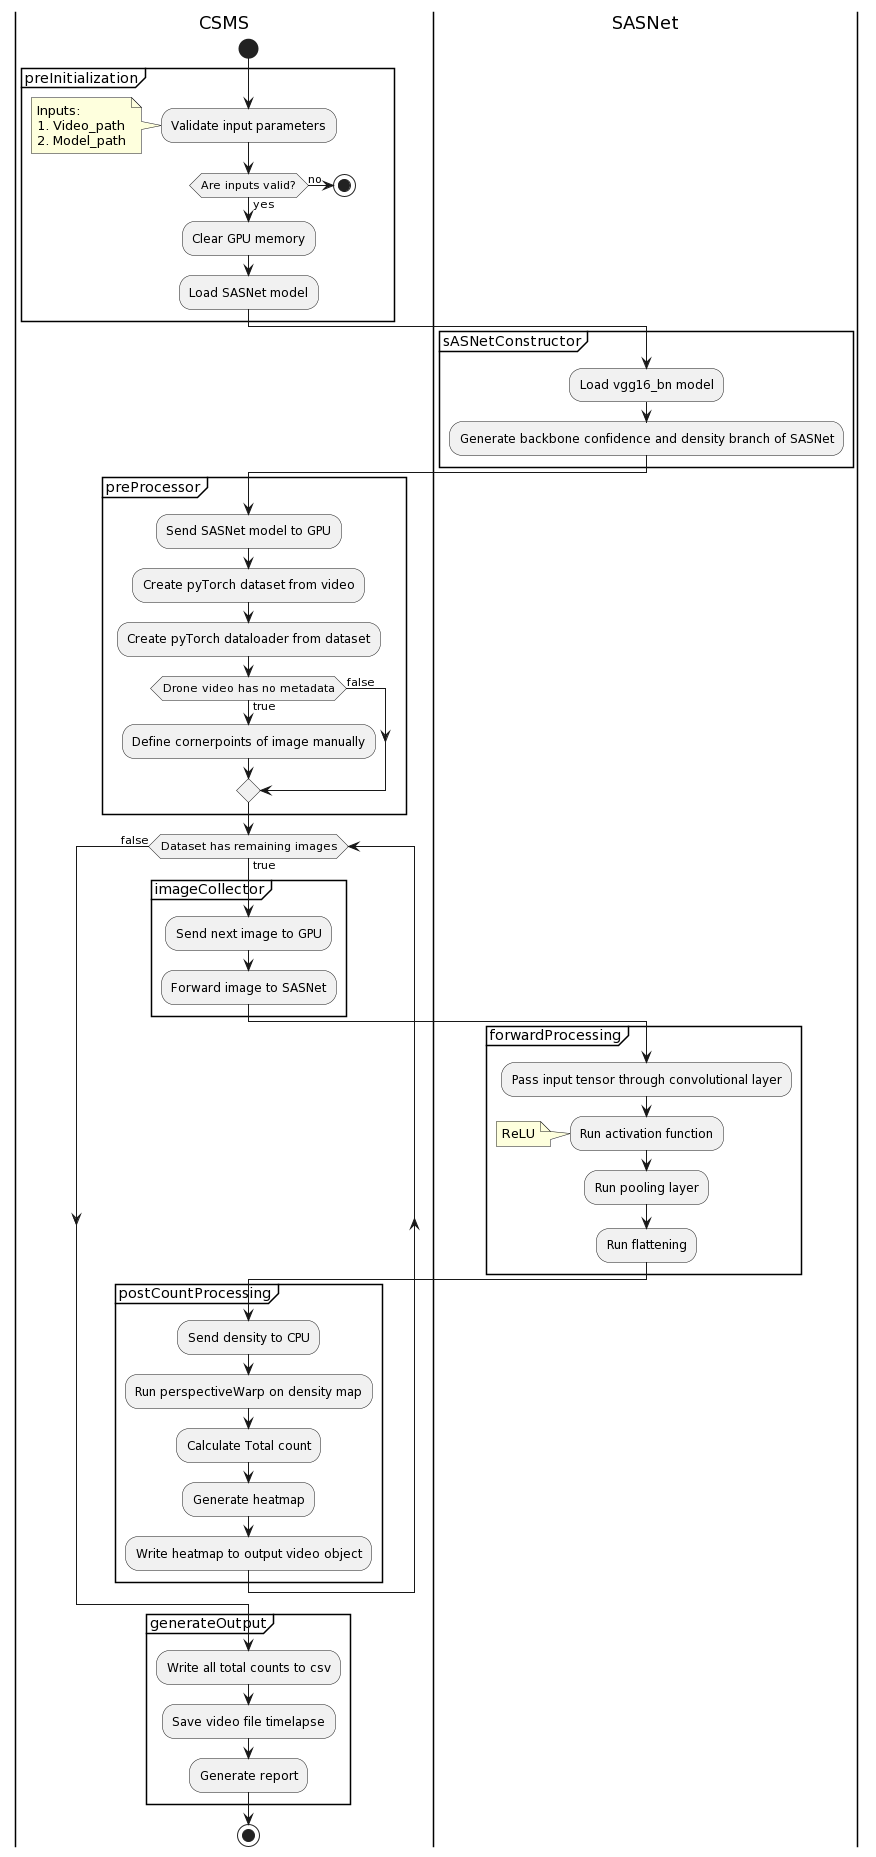
\includegraphics{../images/activity-diagram-1.png}

}

\caption{\label{fig-activity-diagram}Activity diagram depicting flow in
the solution}

\end{figure}

Figure~\ref{fig-activity-diagram} illustrates the flow of the program
through an activity diagram. The diagram was created to obtain a deeper
understanding of the general flow and processes the program goes through
during its runtime. The diagram is split into 2 ``swimlanes'', one lane
for our CSMS system and one lane for the implementation of the SASNet
model. In broad terms, this can also be specified as a CPU and a GPU
lane where our CSMS system handles CPU processing and SASNet focuses on
GPU processing.

As depicted in the diagram, sections of the activities are divided into
partitions to visualise a rough partitioning into classes and for better
readability throughout the diagram. The input is specified as the path
to the pre-trained model and the path to the video for it to run on.

Below is a short run-through of the different partitions.

\begin{enumerate}
\def\labelenumi{\arabic{enumi}.}
\tightlist
\item
  System initialisation and input validation.
\end{enumerate}

The CSMS is initialised and the inputs for the model and video path are
validated

\begin{enumerate}
\def\labelenumi{\arabic{enumi}.}
\setcounter{enumi}{1}
\tightlist
\item
  SASNet model setup and construction.
\end{enumerate}

The SASNet model is loaded together with the VGG16 model which it is
based on. This sets the foundation for subsequent image processing.

\begin{enumerate}
\def\labelenumi{\arabic{enumi}.}
\setcounter{enumi}{2}
\tightlist
\item
  Pre-processing of input data.
\end{enumerate}

Pre-processing involves creating a dataset from the video in pyTorch and
in turn creating a dataloader from this dataset.

\begin{enumerate}
\def\labelenumi{\arabic{enumi}.}
\setcounter{enumi}{3}
\tightlist
\item
  Image processing loop.
\end{enumerate}

The images in the dataloader are iterated through and forwarded to the
SASNet model until the dataloader is empty. Each image is processed
through the different layers to prepare them for post-processing

\begin{enumerate}
\def\labelenumi{\arabic{enumi}.}
\setcounter{enumi}{4}
\tightlist
\item
  Post-processing and result generation.
\end{enumerate}

Following the image processing, the CSMS takes over again. Here density
information is computed, and perspective warping is applied to in turn
generate the correct heatmap for further analysis.

\begin{enumerate}
\def\labelenumi{\arabic{enumi}.}
\setcounter{enumi}{5}
\tightlist
\item
  Output generation and reporting.
\end{enumerate}

All of the outputted data is saved to a file that can be used in the
frontend to form a timelapse and a report, summarising the observations.

\hypertarget{sec-ux}{%
\subsection{Design considerations regarding user
experience}\label{sec-ux}}

For many purposes, a video with a heatmap could be sufficient. However,
to make it possible to satisfy requirements such as functional
requirements 2 and 8 in Table~\ref{tbl-functional-reqs} as well as
non-functional requirement 2 in Table~\ref{tbl-nonfunctional-reqs}, it
was decided to have a user interface. Ideally, by using a frontend with
an API integration to the backend. Alternatively, a frontend where one
may upload the data output from the backend themselves, to analyse the
data further, described as a ``reporting tool'' in functional
requirement 8. The frontend should also have a way of changing the color
scheme of the heatmap for users who have other color preferences or
color blindness.

It is also important to remember that the data produced by the backend
is a means of achieving and solving the overall problem statement.
Keeping the user in mind, they might experience information overload
when looking at a large heatmap with many colors. That is why the
backend is going to downsample the heatmap data to the ratio of 1 pixel
to 1 square meter. This can be upscaled in the front again to improve
the image quality and size, but keeping the ratio of each block on the
image corresponding to one square meter. This makes it easier for the
users to quickly correlate the information with their preexisting
knowledge of service levels (\protect\hyperlink{ref-dahl2023crowd}{Dahl
2023}). Service levels are usually described in people per square meter.
Limiting the heatmap color scale to cap out at \textgreater5 people per
square meter as this is when the density could become worrisome.

\hypertarget{the-cyber-physical-system}{%
\subsection{The Cyber-Physical System}\label{the-cyber-physical-system}}

Our system could in a cyber-physical aspect integrate the automated
sensors (cameras) within a closed network IoT framework to monitor the
crowd density. The sensors collect data in real-time, which is then
processed and analysed centrally.

Despite the automated data collection, decision-making remains a
human-driven process, with safety experts interpreting the sensor
outputs. The interface for this system is user-friendly described in
Section~\ref{sec-ux}, and could offer real-time visualisations of crowd
dynamics. Future enhancements may explore more automated decision-making
capabilities. See Section~\ref{sec-perspective}.

It is necessary to implement an IoT framework to implement
non-functional requirements 6 and 7 in
Section~\ref{sec-non-functional-requirements}. It would also be
necessary in order to implement functional requirement 12 in
Section~\ref{sec-functional-requirements}. However, this requirement is
not part of the project scope as it is a ``will not'' in the MoSCoW
prioritisation.

\newpage{}

\hypertarget{sec-implementation}{%
\section{Implementation}\label{sec-implementation}}

This section is going to describe the implementation of as many designed
elements as possible within the timeframe, following the prioritisation
in Section~\ref{sec-analysis} and the design choices made in
Section~\ref{sec-design}.

\hypertarget{data-collection-and-preparation}{%
\subsection{Data Collection and
Preparation}\label{data-collection-and-preparation}}

To implement this project it was necessary to gather useful evaluation
data. For this project, that is video security footage and drone
footage. Our collaborative partner Event Safety was very helpful in
letting us gather this data at their 2 festivals, ``Smukfest'' and
``Grøn''. This was done 1-2 months before the project started since this
is when the festivals were held. This means that we gathered the data
before completing the research on crowd counting and computer vision. It
did pose a challenge to collect the data before knowing exactly what
type of data was needed. For these reasons, we collected many types of
data, including:

\begin{enumerate}
\def\labelenumi{\arabic{enumi}.}
\item
  Drone footage from ``Grøn'' at an altitude of 25-50 meters from the
  entrance
\item
  Drone footage from ``Grøn'' at an altitude of 25-50 meters of the
  concerts and end of concerts
\item
  GoPro footage from ``Grøn'' at an altitude of 2-5 meters from the
  entrance
\item
  Security camera footage from ``Smukfest at an altitude of
  approximately 10-15 meters from the center of the stage.
\item
  Security camera footage from ``Smukfest'' at various heights from bars
  and paths
\end{enumerate}

What turned out to be most useful was option number 2 and option number
4. Having a perspective from a higher altitude means that more people
are clearly visible and also minimises distortion when warping for
perspective correction. Having an even higher resolution from a higher
altitude could also increase the accuracy of the predictions. The
resolution of the drone footage was 1080p. Having a higher resolution
could limit the video compression artifacts. The camera options were
discussed with our secondary partner PhaseOne. They have experience with
ultra-high-resolution top-down drone footage. This could be an option
for future endeavors, which will be discussed in
Section~\ref{sec-perspective} of this report.

While we, with the help of a certified drone pilot, collected the
footage from ``Grøn'' ourselves, the security footage from ``Smukfest''
was collected by Event Safety. For this, we created a technical
specification with our requirements for the footage at the time. This
can be read in Section~\ref{sec-appendices}.

\hypertarget{sec-backend}{%
\subsection{Backend implementation}\label{sec-backend}}

This section will describe the implementation of the backend. The
backend is where the majority of the expensive computing is going to be
performed, as well as the use of SASNet and expensive computer vision
functions.

To create an efficient, manageable and scaleable backend, an
object-oriented design in Python was chosen. In this section, we will
look at the responsibilities of each class and how they interact to
fulfill the requirements. A class diagram of the backend is shown below
in Figure~\ref{fig-class-backend}.

\begin{figure}

{\centering 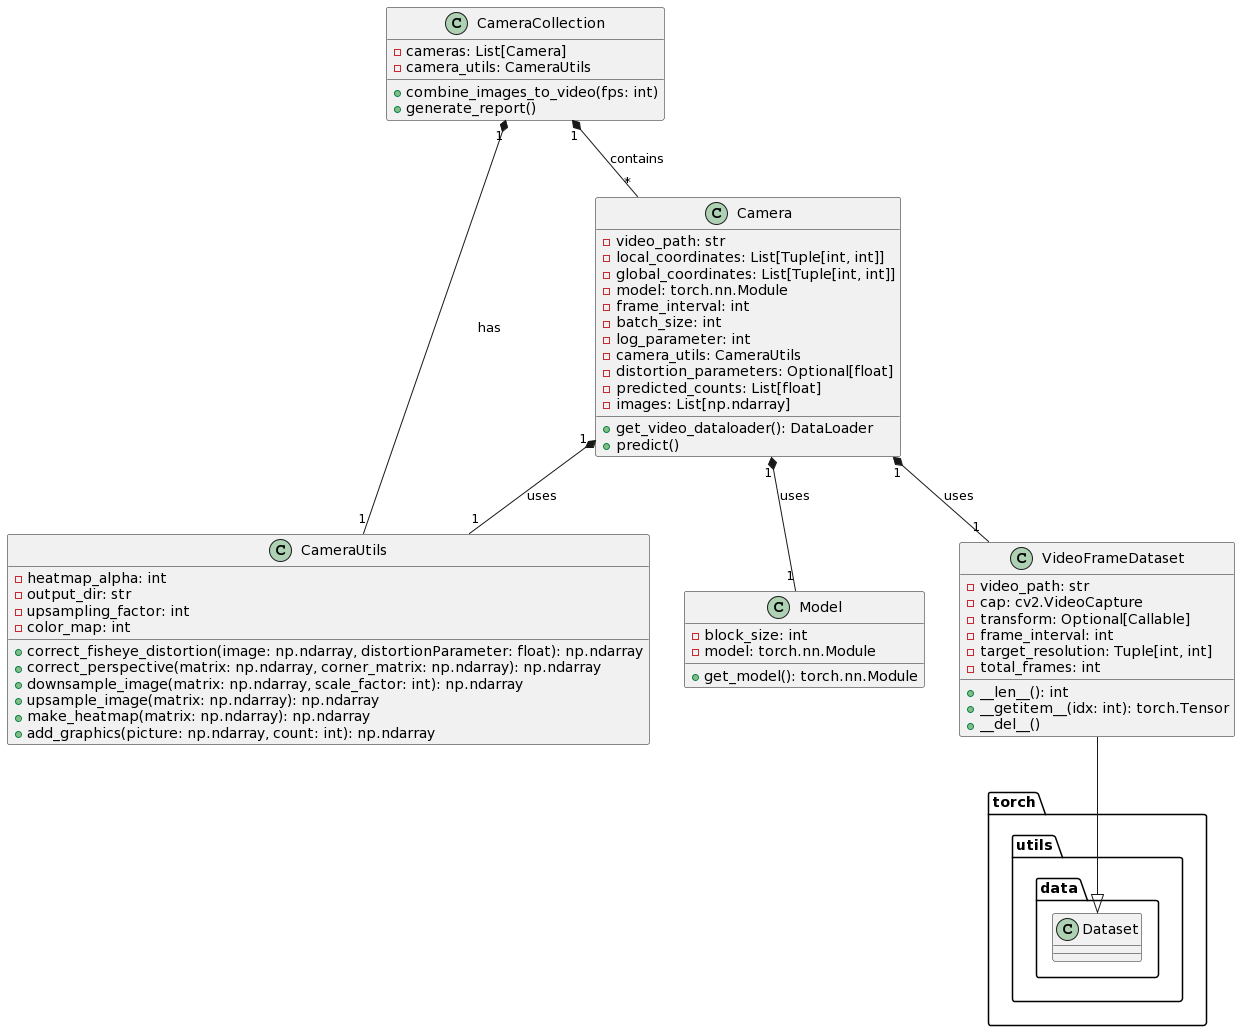
\includegraphics{../images/class-backend.png}

}

\caption{\label{fig-class-backend}Class diagram depicting the structure
of the backend}

\end{figure}

In this section, we will refer back to
Section~\ref{sec-functional-requirements} to show the implementation of
a few requirements.

\hypertarget{sec-classes}{%
\subsubsection{Backend class structure}\label{sec-classes}}

Referring to Figure~\ref{fig-class-backend}, we see that the backend
mainly consists of 5 classes:

\begin{enumerate}
\def\labelenumi{\arabic{enumi}.}
\tightlist
\item
  VideoFrameDataset
\item
  ModelWrapper
\item
  Camera
\item
  CameraUtils
\item
  CameraCollection
\end{enumerate}

The system is built on the OOP paradigm for easier scalability to
additional cameras in the future. The responsibilities of the 5 main
classes are described in the following:

\begin{itemize}
\item
  VideoFrameDataset VideoFrameDataset takes the video input and converts
  it to the type of Dataset. This allows us to segment the video based
  on a frame interval for easier manipulation later on. Here, the size
  of the video is also set to a specific resolution based on passed
  parameters and resized using the cv2.resize() function. The class
  returns the frames of the video in a Dataset.\\
\item
  ModelWrapper ModelWrapper loads the model from the SASNet repository
  into a Model object with relevant parameters. The class contains a
  get\_model() method for fetching the model in the other classes.\\
\item
  Camera The Camera class contains the main predict() method. This
  method is explained in Section~\ref{sec-crowdcount-implement}. Beyond
  the predict() method, the class gets the Dataset from earlier and
  passes it to a Dataloader which the predict method fetches. When the
  predict() method has run, it returns a heatmap for processing in the
  frontend.\\
\item
  CameraUtils The CameraUtils class is a large collection of methods
  used in the Camera and CameraUtils classes. These methods include, but
  are not limited to: correct\_fisheye\_distortion(),
  correct\_perspective(), downsample\_image(), upsample\_image() and
  make\_heatmap(). All of these methods are used in the predict() method
  in the camera class and aid in manipulating the frames of the video
  for better and more accurate crowd counting.\\
\item
  CameraCollection As the main goal of this project is to help improve
  crowd safety management, the implementation of software that can
  handle multiple cameras at once is important. The CameraCollection
  class does just that. The other main responsibility of this class is
  the conversion from frames in a Dataset back to a video timelapse. The
  class takes all of the frames and combines them into a video with a
  set amount of frames per second(FPS) and then saves the video to the
  .avi format.\\
\end{itemize}

\hypertarget{sec-environment}{%
\subsubsection{Environment setup}\label{sec-environment}}

Setting up an environment for machine learning in Python is not trivial.
It is a requirement to have access to a NVIDIA GPU to take advantage of
the CUDA toolkit in PyTorch. This opens up GPU acceleration which
enables a performance boost rather than running the CNN models on the
CPU. Furthermore, the SASNet open-source project was built for Python
3.6.8 and PyTorch \textgreater= 1.5.0
(\protect\hyperlink{ref-sasnet}{Song et al. 2021}). All of this has to
taken into account when setting up the environment. We created a bash
script which can be seen in Section~\ref{sec-appendices} with the
following responsibilities to initiate the environment:

\begin{itemize}
\item
  Initiating and cloning Git submodules
\item
  Installing necessary Ubuntu packages
\item
  Installing necessary Python installation
\item
  Installing Python package manager (PIP)
\item
  Installing all Python package dependencies
\end{itemize}

\hypertarget{ucloud-service}{%
\subsubsection{UCloud service}\label{ucloud-service}}

SDU provides a cloud computing service for faculty members through
\href{https://escience.sdu.dk/index.php/national-hpc-systems/}{eScience}.
Our supervisor applied through this site for a cloud computing resource
with 50 GPU hours. The project was granted 100 GB storage and the
``u1-gpu @ DeiC Interactive HPC (SDU)'' server. In UCloud we used the
application ``Coder CUDA'' to run the project. The bash script from
Section~\ref{sec-environment} is run to initialise the environment.

\hypertarget{sasnet-model-adaptation}{%
\subsubsection{SASNet Model Adaptation}\label{sasnet-model-adaptation}}

The SASNet model is loaded using pre-trained weights and biases for the
underlying vgg16\_bn model trained on ImageNet
(\protect\hyperlink{ref-sasnet}{Song et al. 2021}). This allows SASNet
to more efficiently identify image features with low memory usage.
Furthermore, the SASNet weights and bias fine-tunings are loaded into
the model which has been trained on the ShanghaiTech Part A dataset.

\hypertarget{sec-req-imp}{%
\subsubsection{Implementation of requirements}\label{sec-req-imp}}

This section about the backend implementation will take a closer look at
how functional requirements 1 and 4 were implemented.

\hypertarget{sec-crowdcount-implement}{%
\paragraph{Implementing crowd counting}\label{sec-crowdcount-implement}}

This section describes the implementation of functional requirement 1:
``\emph{The system must be able to count the number of people in the
crowd with the precision required by the user base.}''

To count the people in a crowd, the SASNet crowd counting model
mentioned in Section~\ref{sec-model-selection} was implemented in the
backend. This is done in the model\_wrapper.py class. The model\_wrapper
class has a get\_model() method that returns the model for use in the
camera class.

Before we can use the model on our data, it needs to be preprocessed. As
the SASNet model is made for singular images, converting the input
videos to an image-based format is needed. This is done using the Python
torch.utils.dataset class. This iterable dataset allows for loading a
frame interval from a video into an array of images using cv2. Using
cv2, we are also able to resize the video to a specified resolution for
easier handling. Once a specified frame interval, resolution and other
parameters for the video are defined, it is ready for processing and
gets loaded by the camera class.

\begin{Shaded}
\begin{Highlighting}[]
\KeywordTok{def}\NormalTok{ predict(}\VariableTok{self}\NormalTok{) }\OperatorTok{{-}\textgreater{}} \VariableTok{None}\NormalTok{:}
\NormalTok{torch.cuda.empty\_cache()}
\NormalTok{gc.collect()}

\NormalTok{dataloader }\OperatorTok{=} \VariableTok{self}\NormalTok{.get\_video\_dataloader()}

\ControlFlowTok{for}\NormalTok{ img }\KeywordTok{in}\NormalTok{ dataloader:}
\NormalTok{  img }\OperatorTok{=}\NormalTok{ img.cuda()}

  \ControlFlowTok{with}\NormalTok{ torch.no\_grad():}
    \VariableTok{self}\NormalTok{.model.}\BuiltInTok{eval}\NormalTok{()}
\NormalTok{    pred\_map }\OperatorTok{=} \VariableTok{self}\NormalTok{.model(img)}
\NormalTok{  pred\_map }\OperatorTok{=}\NormalTok{ pred\_map.data.cpu().numpy()}

  \ControlFlowTok{for}\NormalTok{ i\_img }\KeywordTok{in} \BuiltInTok{range}\NormalTok{(pred\_map.shape[}\DecValTok{0}\NormalTok{]):}
\NormalTok{    pred\_cnt }\OperatorTok{=}\NormalTok{ np.}\BuiltInTok{sum}\NormalTok{(pred\_map[i\_img]) }\OperatorTok{/} \VariableTok{self}\NormalTok{.log\_parameter}
    \VariableTok{self}\NormalTok{.predicted\_counts.append(pred\_cnt)}

\NormalTok{    grayscale\_map }\OperatorTok{=}\NormalTok{ pred\_map[i\_img][}\DecValTok{0}\NormalTok{] }\CommentTok{\# Extract the first channel (grayscale) from the density map}

    \ControlFlowTok{if} \VariableTok{self}\NormalTok{.distortion\_parameters }\KeywordTok{and} \BuiltInTok{len}\NormalTok{(}\VariableTok{self}\NormalTok{.distortion\_parameters) }\OperatorTok{\textgreater{}} \DecValTok{0}\NormalTok{:}
\NormalTok{      undistorted\_map }\OperatorTok{=} \VariableTok{self}\NormalTok{.camera\_utils.correct\_fisheye\_distortion(grayscale\_map, }\VariableTok{self}\NormalTok{.distortion\_parameters[}\DecValTok{0}\NormalTok{])}
    \ControlFlowTok{else}\NormalTok{:}
\NormalTok{      undistorted\_map }\OperatorTok{=}\NormalTok{ grayscale\_map}

\NormalTok{    corrected\_map }\OperatorTok{=} \VariableTok{self}\NormalTok{.camera\_utils.correct\_perspective(undistorted\_map, }\VariableTok{self}\NormalTok{.local\_coordinates)}

\NormalTok{    width\_after }\OperatorTok{=} \VariableTok{self}\NormalTok{.global\_coordinates[}\DecValTok{3}\NormalTok{][}\DecValTok{0}\NormalTok{] }\OperatorTok{{-}} \VariableTok{self}\NormalTok{.global\_coordinates[}\DecValTok{0}\NormalTok{][}\DecValTok{0}\NormalTok{]}
\NormalTok{    scale\_factor }\OperatorTok{=} \BuiltInTok{int}\NormalTok{(corrected\_map.shape[}\DecValTok{1}\NormalTok{] }\OperatorTok{/}\NormalTok{ width\_after)}

\NormalTok{    downsampled\_map }\OperatorTok{=} \VariableTok{self}\NormalTok{.camera\_utils.downsample\_image(corrected\_map, scale\_factor)}

\NormalTok{    upsampled\_map }\OperatorTok{=} \VariableTok{self}\NormalTok{.camera\_utils.upsample\_image(downsampled\_map)}

\NormalTok{    heatmap }\OperatorTok{=} \VariableTok{self}\NormalTok{.camera\_utils.make\_heatmap(upsampled\_map)}

    \VariableTok{self}\NormalTok{.images.append(heatmap)}
\end{Highlighting}
\end{Shaded}

After loading both the model and dataset, the Camera.predict() method
seen above is called. The predict method first clears the garbage
collector and empties cached GPU memory. Each image in the dataset is
then iterated over and assigned to PyTorch.Cuda, sending it to be
processed by the GPU. The model now infers the image and the resulting
density map is assigned to the pred\_map variable.

After assigning the density maps several post-processing steps happen.
First, the predicted count is calculated by the SASnet model. How this
works is explained in simple terms in
Section~\ref{sec-design-crowdcounting}.

Secondly, the method checks if parameters for fisheye correction are
passed. If true, the program applies fisheye correction from cv2 and
continues, otherwise, this part is skipped.

Third, the first color channel (grayscale) is extracted for further
processing. Following this, perspective correction and aggregate
downsampling are performed. Upsampling using ``nearest'' interpolation
is also applied if the upsampling factor is different from 1. For use
with the frontend, the upsampling factor should be 1 as the upsampling
should be done in the frontend. More on this in
Section~\ref{sec-correction}. It is important to note that crowd
counting is done before perspective correction, as the model is unable
to count accurately on the warped image.

Finally, the corrected map is converted into a heatmap using the
make\_heatmap() method from CameraUtils if a heatmap color scheme is
provided. For use with the frontend this should not be provided as the
heatmap will be applied in the frontend. The resulting image is returned
to be written to a video file.

In CameraUtils we also find the add\_graphics() method, simply adding a
small graphic to the image with the predicted count if it is wanted to
use the video without the frontend.

\hypertarget{sec-correction}{%
\paragraph{Implementing the functions to create
heatmaps}\label{sec-correction}}

This section describes the implementation of functional requirement 4:
``\emph{The system should be able to calculate the physical density of
humans pr. area unit}''

Before explaining how functional requirement 4 is implemented, a look at
how downsampling and perspective correction work in our system is
needed.

When a camera is instantiated in the main class, a set of local and
global coordinates are passed with it, as seen in the code snippet
below.

\begin{Shaded}
\begin{Highlighting}[]
\NormalTok{local\_coords }\OperatorTok{=}\NormalTok{ [(}\DecValTok{797}\NormalTok{, }\DecValTok{293}\NormalTok{), (}\DecValTok{287}\NormalTok{, }\DecValTok{653}\NormalTok{), (}\DecValTok{1761}\NormalTok{, }\DecValTok{1040}\NormalTok{), (}\DecValTok{1734}\NormalTok{, }\DecValTok{411}\NormalTok{)]}
\NormalTok{global\_coords }\OperatorTok{=}\NormalTok{ [(}\DecValTok{0}\NormalTok{, }\DecValTok{0}\NormalTok{), (}\DecValTok{0}\NormalTok{, }\DecValTok{80}\NormalTok{), (}\DecValTok{100}\NormalTok{, }\DecValTok{80}\NormalTok{), (}\DecValTok{100}\NormalTok{, }\DecValTok{0}\NormalTok{)]}
\end{Highlighting}
\end{Shaded}

The local coordinates are taken from the frame of the video, depicting
the area we want to analyse and correct. The global coordinates are the
real-world distances between points, taken from various land surveys of
the different festivals provided by our partner at Event Safety. Using
these coordinates as measurements we can correct the perspective of each
frame for accurate density heatmaps based on physical distances.

Perspective correction is done using the cv2 method which takes the
extracted grayscale map from earlier and the local coordinates from the
frame. First, the transformation matrix M is calculated using the
original input coordinates and the desired output coordinates. See
Figure~\ref{fig-transformation-matrix}.

\begin{figure}

{\centering 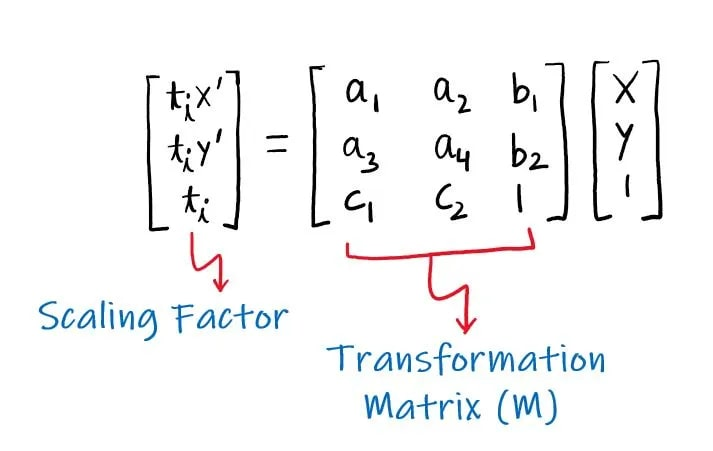
\includegraphics{../images/perspec-trans-matrix.jpg}

}

\caption{\label{fig-transformation-matrix}Depiction of transformation
matrix and scale factor (From
\protect\hyperlink{ref-cv2-warpperspective}{The AI Learner, n.d.})}

\end{figure}

After finding the transformation matrix, the operation is performed on
the section of the image defined in local\_coordinates, using the
warpPerspective() method from cv2. The process can be seen in
Figure~\ref{fig-perspective-transformation}.

\begin{figure}

{\centering 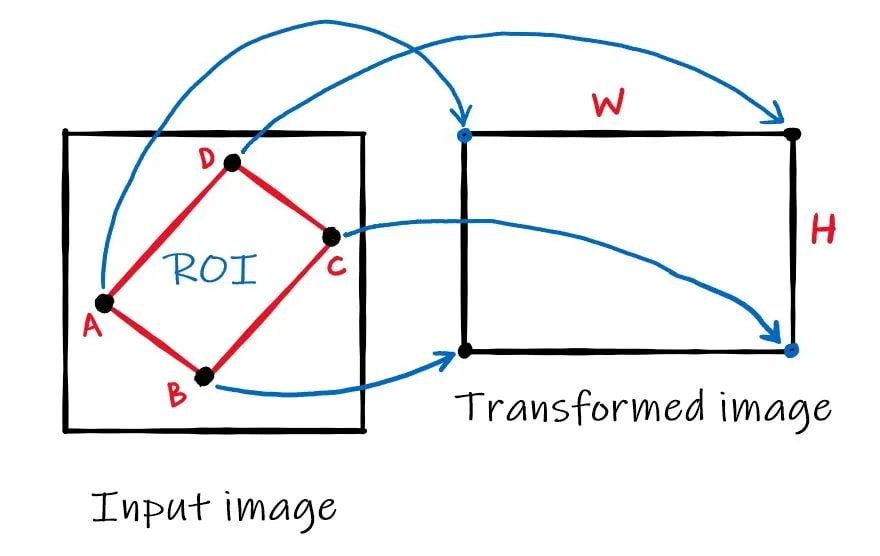
\includegraphics{../images/perspective-transformation-visual.jpg}

}

\caption{\label{fig-perspective-transformation}Depiction of perspective
correction from The AI Learner
(\protect\hyperlink{ref-cv2-warpperspective}{n.d.})}

\end{figure}

The code snippet for perspective correction is also found below:

\begin{Shaded}
\begin{Highlighting}[]
 \KeywordTok{def}\NormalTok{ correct\_perspective(}\VariableTok{self}\NormalTok{, matrix: np.ndarray, corner\_matrix: np.ndarray) }\OperatorTok{{-}\textgreater{}}\NormalTok{ np.ndarray:}
\NormalTok{  pt\_A }\OperatorTok{=}\NormalTok{ corner\_matrix[}\DecValTok{0}\NormalTok{]}
\NormalTok{  pt\_B }\OperatorTok{=}\NormalTok{ corner\_matrix[}\DecValTok{1}\NormalTok{]}
\NormalTok{  pt\_C }\OperatorTok{=}\NormalTok{ corner\_matrix[}\DecValTok{2}\NormalTok{]}
\NormalTok{  pt\_D }\OperatorTok{=}\NormalTok{ corner\_matrix[}\DecValTok{3}\NormalTok{]}

\NormalTok{  width\_AD }\OperatorTok{=}\NormalTok{ np.sqrt(((pt\_A[}\DecValTok{0}\NormalTok{] }\OperatorTok{{-}}\NormalTok{ pt\_D[}\DecValTok{0}\NormalTok{]) }\OperatorTok{**} \DecValTok{2}\NormalTok{) }\OperatorTok{+} 
\NormalTok{  ((pt\_A[}\DecValTok{1}\NormalTok{] }\OperatorTok{{-}}\NormalTok{ pt\_D[}\DecValTok{1}\NormalTok{]) }\OperatorTok{**} \DecValTok{2}\NormalTok{))}

\NormalTok{  width\_BC }\OperatorTok{=}\NormalTok{ np.sqrt(((pt\_B[}\DecValTok{0}\NormalTok{] }\OperatorTok{{-}}\NormalTok{ pt\_C[}\DecValTok{0}\NormalTok{]) }\OperatorTok{**} \DecValTok{2}\NormalTok{) }\OperatorTok{+} 
\NormalTok{  ((pt\_B[}\DecValTok{1}\NormalTok{] }\OperatorTok{{-}}\NormalTok{ pt\_C[}\DecValTok{1}\NormalTok{]) }\OperatorTok{**} \DecValTok{2}\NormalTok{))}

\NormalTok{  maxWidth }\OperatorTok{=} \BuiltInTok{max}\NormalTok{(}\BuiltInTok{int}\NormalTok{(width\_AD), }\BuiltInTok{int}\NormalTok{(width\_BC))}


\NormalTok{  height\_AB }\OperatorTok{=}\NormalTok{ np.sqrt(((pt\_A[}\DecValTok{0}\NormalTok{] }\OperatorTok{{-}}\NormalTok{ pt\_B[}\DecValTok{0}\NormalTok{]) }\OperatorTok{**} \DecValTok{2}\NormalTok{) }\OperatorTok{+} 
\NormalTok{  ((pt\_A[}\DecValTok{1}\NormalTok{] }\OperatorTok{{-}}\NormalTok{ pt\_B[}\DecValTok{1}\NormalTok{]) }\OperatorTok{**} \DecValTok{2}\NormalTok{))}

\NormalTok{  height\_CD }\OperatorTok{=}\NormalTok{ np.sqrt(((pt\_C[}\DecValTok{0}\NormalTok{] }\OperatorTok{{-}}\NormalTok{ pt\_D[}\DecValTok{0}\NormalTok{]) }\OperatorTok{**} \DecValTok{2}\NormalTok{) }\OperatorTok{+} 
\NormalTok{  ((pt\_C[}\DecValTok{1}\NormalTok{] }\OperatorTok{{-}}\NormalTok{ pt\_D[}\DecValTok{1}\NormalTok{]) }\OperatorTok{**} \DecValTok{2}\NormalTok{))}

\NormalTok{  maxHeight }\OperatorTok{=} \BuiltInTok{max}\NormalTok{(}\BuiltInTok{int}\NormalTok{(height\_AB), }\BuiltInTok{int}\NormalTok{(height\_CD))}

\NormalTok{  input\_pts }\OperatorTok{=}\NormalTok{ np.float32([pt\_A, pt\_B, pt\_C, pt\_D])}
\NormalTok{  output\_pts }\OperatorTok{=}\NormalTok{ np.float32([[}\DecValTok{0}\NormalTok{, }\DecValTok{0}\NormalTok{],}
\NormalTok{                          [}\DecValTok{0}\NormalTok{, maxHeight }\OperatorTok{{-}} \DecValTok{1}\NormalTok{],}
\NormalTok{                          [maxWidth }\OperatorTok{{-}} \DecValTok{1}\NormalTok{, maxHeight }\OperatorTok{{-}} \DecValTok{1}\NormalTok{],}
\NormalTok{                          [maxWidth }\OperatorTok{{-}} \DecValTok{1}\NormalTok{, }\DecValTok{0}\NormalTok{]])}
\end{Highlighting}
\end{Shaded}

When the perspective of the frame is corrected, the image is then
downsampled to reduce information overload and increase the crowd
overview by having each ``pixel'' of the frame correlate to 1 square
meter in real life based on the global coordinates. After this, the
image is then upsampled again so the data is still readable but not
overwhelming.

The code for the downsample\_image() method is seen below:

\begin{Shaded}
\begin{Highlighting}[]
 \KeywordTok{def}\NormalTok{ downsample\_image(}\VariableTok{self}\NormalTok{, matrix: np.ndarray, scale\_factor: }\BuiltInTok{int}\NormalTok{) }\OperatorTok{{-}\textgreater{}}\NormalTok{ np.ndarray:}
    \CommentTok{\# Calculate the dimensions of the downscaled array with padding}
\NormalTok{  new\_height }\OperatorTok{=}\NormalTok{ matrix.shape[}\DecValTok{0}\NormalTok{] }\OperatorTok{//}\NormalTok{ scale\_factor }\OperatorTok{+}\NormalTok{ (matrix.shape[}\DecValTok{0}\NormalTok{] }\OperatorTok{\%}\NormalTok{ scale\_factor }\OperatorTok{\textgreater{}} \DecValTok{0}\NormalTok{)}
\NormalTok{  new\_width }\OperatorTok{=}\NormalTok{ matrix.shape[}\DecValTok{1}\NormalTok{] }\OperatorTok{//}\NormalTok{ scale\_factor }\OperatorTok{+}\NormalTok{ (matrix.shape[}\DecValTok{1}\NormalTok{] }\OperatorTok{\%}\NormalTok{ scale\_factor }\OperatorTok{\textgreater{}} \DecValTok{0}\NormalTok{)}

  \CommentTok{\# Initialize the downscaled array with zeros}
\NormalTok{  downscaled\_array }\OperatorTok{=}\NormalTok{ np.zeros((new\_height, new\_width), dtype}\OperatorTok{=}\NormalTok{matrix.dtype)}

  \CommentTok{\# Iterate through the downscaled array and calculate the sum of the pixels}
  \ControlFlowTok{for}\NormalTok{ i }\KeywordTok{in} \BuiltInTok{range}\NormalTok{(new\_height):}
    \ControlFlowTok{for}\NormalTok{ j }\KeywordTok{in} \BuiltInTok{range}\NormalTok{(new\_width):}
\NormalTok{      row\_start }\OperatorTok{=}\NormalTok{ i }\OperatorTok{*}\NormalTok{ scale\_factor}
\NormalTok{      row\_end }\OperatorTok{=} \BuiltInTok{min}\NormalTok{((i }\OperatorTok{+} \DecValTok{1}\NormalTok{) }\OperatorTok{*}\NormalTok{ scale\_factor, matrix.shape[}\DecValTok{0}\NormalTok{])}
\NormalTok{      col\_start }\OperatorTok{=}\NormalTok{ j }\OperatorTok{*}\NormalTok{ scale\_factor}
\NormalTok{      col\_end }\OperatorTok{=} \BuiltInTok{min}\NormalTok{((j }\OperatorTok{+} \DecValTok{1}\NormalTok{) }\OperatorTok{*}\NormalTok{ scale\_factor, matrix.shape[}\DecValTok{1}\NormalTok{])}
\NormalTok{      downscaled\_array[i, j] }\OperatorTok{=}\NormalTok{ np.}\BuiltInTok{sum}\NormalTok{(matrix[row\_start:row\_end, col\_start:col\_end])}

  \ControlFlowTok{return}\NormalTok{ downscaled\_array}
\end{Highlighting}
\end{Shaded}

This leaves us with the steps condensed into:

\begin{enumerate}
\def\labelenumi{\arabic{enumi}.}
\tightlist
\item
  Correct the perspective of the heatmap based on global coordinates.
\item
  Downsample the corrected greyscale heatmap to ensure that each pixel
  in a given frame corresponds to area units - square meters in this
  case.
\item
  Upsample the downsampled image for better readability while still
  maintaining a linear relationship between pixels and area units. (This
  is only done if the frontend is not used)
\end{enumerate}

After the complete image processing and the steps above are complete,
the greyscale heatmap is uploaded to the frontend. Here the pixel sum of
the entire image is divided by the amount of pixels to find the density.
This is due to the density of people being represented by pixel density
as explained in Section~\ref{sec-design-crowdcounting}.

\newpage{}

\hypertarget{frontend}{%
\subsection{Frontend}\label{frontend}}

To create a flexible user interface, the output data was stripped of all
post-processing artifacts (heatmap, scale, count and other text) as this
would now be calculated in the frontend. The frontend is created using
\href{https://wiki.qt.io/Qt_for_Python}{Qt for Python} to allow for
cross-platform compatibility, to have access to video playback
components and the Python OpenCV module to allow for preprocessing of
the video. There are 3 main widgets in the frontend. The main
VideoPlayer widget that has buttons to upload the video, clear mask and
change heatmap color scheme. The InfoWidget that displays textual data
such as the count, count in the selection, density, density in selection
and time passed. The FloatingOverlay that is an overlay that follows the
size and position of the VideoPlayer where the user can draw a polygon
to define an area on the video that should be counted, as defined in
functional requirement 2 in Table~\ref{tbl-functional-reqs}.

\begin{figure}

{\centering 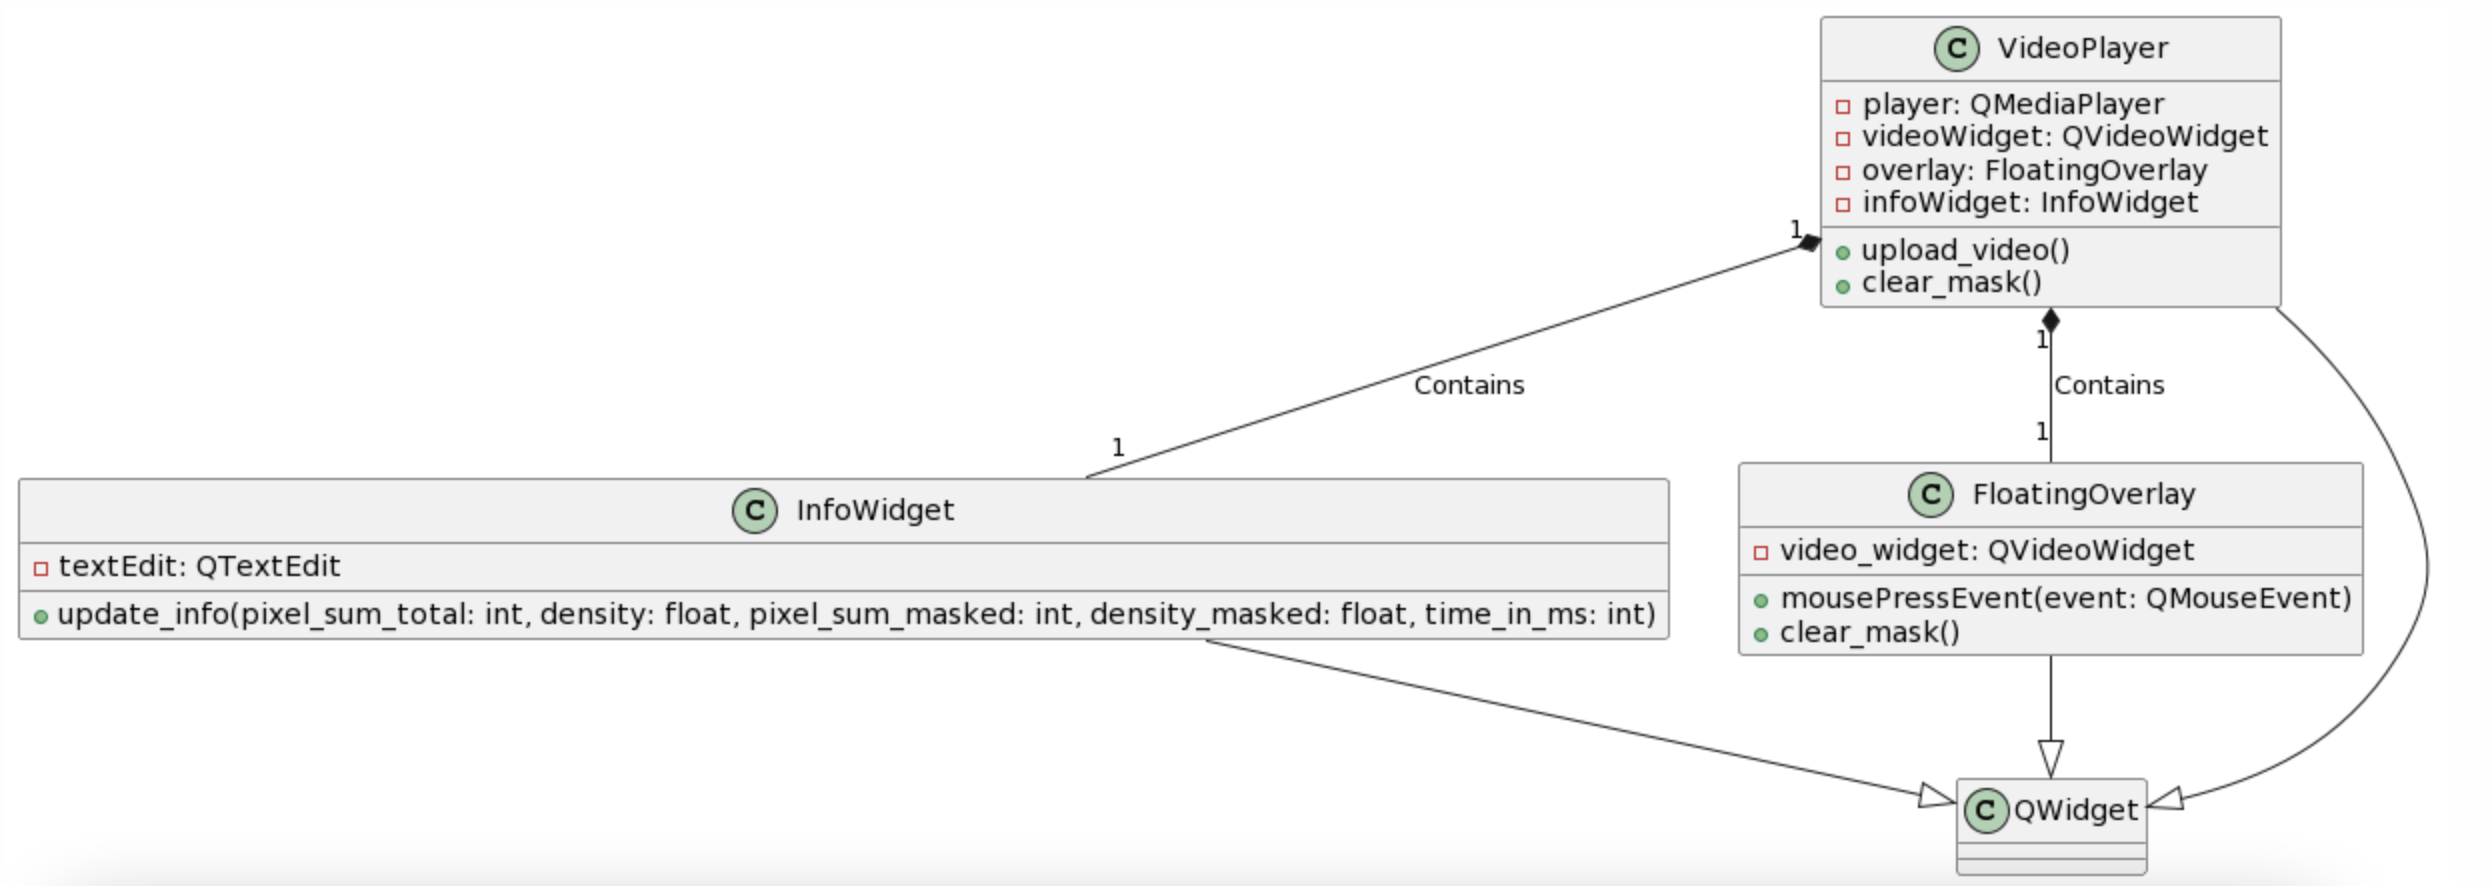
\includegraphics{../images/class-diagram-frontend.png}

}

\caption{\label{fig-fcd}Simplified class diagram depicting the structure
of the frontend}

\end{figure}

A simplified version of this structure can be seen in
Figure~\ref{fig-fcd} and the full diagram with all methods and
attributes can be seen in the appendix. The VideoPlayer calls a
preprocess function that adds the selected heatmap and upscales the
downsampled video before sending it to the QVideoWidget. A density scale
is also created after the video has been uploaded. All of this is done
using OpenCV. This is done in accordance with functional requirement 3
in Table~\ref{tbl-functional-reqs}.

\hypertarget{integeration}{%
\subsection{Integeration}\label{integeration}}

Although a proper API between the frontend and backend was described in
the component diagram, Figure~\ref{fig-component-diagram}, it has not
been a priority of the project and has thus not been developed. Further
development could allow for direct upload to the backend processing unit
from the frontend. Instead as of right now, all video content must be
uploaded to UCloud for processing which then produces an output video
file in the .avi file format that can be read and processed properly by
the frontend. Pairing this file with a metadata file containing the
input parameters to the backend such as frame sampling interval could
also be useful so these parameters become dynamic in the frontend. The
metadata file could also contain total counts and average densities over
time, so these expensive operations do not have to be unnecessarily
recalculated in the frontend.

\hypertarget{optimisation-and-performance}{%
\subsection{Optimisation and
Performance}\label{optimisation-and-performance}}

For two main reasons, it is necessary to limit the compute resource
usage:

\begin{enumerate}
\def\labelenumi{\arabic{enumi}.}
\item
  This project is using limited GPU and compute resources provided by
  UCloud. Computer vision and CNN's can be very GPU intensive, so it is
  in the project's interest to limit the GPU memory consumption as this
  was found to be the largest resource bottleneck.
\item
  For the CSMS to be scalable to (near) real-time evaluation
  performance, it makes sense to limit the use of computing power as
  much as possible.
\end{enumerate}

According to Contributors (\protect\hyperlink{ref-pytorch}{2023}),
\href{https://pytorch.org/docs/stable/generated/torch.no_grad.html}{disabling
gradient calculation} is useful for lowering memory usage when using a
model for inference. This fits the use case and greatly reduces memory
usage. This was done in the following way:

\begin{Shaded}
\begin{Highlighting}[]
\NormalTok{img }\OperatorTok{=}\NormalTok{ img.cuda()}
\ControlFlowTok{with}\NormalTok{ torch.no\_grad():}
\NormalTok{  model.}\BuiltInTok{eval}\NormalTok{()}
\NormalTok{  pred\_map }\OperatorTok{=}\NormalTok{ model(img)}
\NormalTok{pred\_map }\OperatorTok{=}\NormalTok{ pred\_map.data.cpu().numpy()}
\end{Highlighting}
\end{Shaded}

Here the image tensor is first sent to the NVIDIA GPU using img.cuda().
Gradient calculations are then disabled for the inference, and the model
is set to eval mode. These two reduce the GPU memory usage. Finally,
after the inference is run and the predicition\_map is calculated, the
tensor data is sent to the CPU and the tensor is converted to a NumPy
matrix (an image). This way limits the time that the tensor spends in
the GPU greatly, as well as reducing memory usage.

\newpage{}

\hypertarget{sec-validation-verification}{%
\section{Validation and
Verification}\label{sec-validation-verification}}

Since this project is a proof of concept, automated unit tests and
integration tests are not as favored as user tests and similar. Because
of the innovative nature of the product, validation of the idea is more
important than verification. Testing this system relies on making sure
that it is useful and understandable to those who need it. To accomplish
these tests, we decided to perform both manual count comparisons and get
the opinions of Event Safety security personnel and professionals about
our project and its viability.

\hypertarget{sec-accuracy}{%
\subsection{Accuracy of Crowd Count}\label{sec-accuracy}}

To test the accuracy of the model, a manual test was conducted on a
small area of the video.

\begin{figure}

{\centering 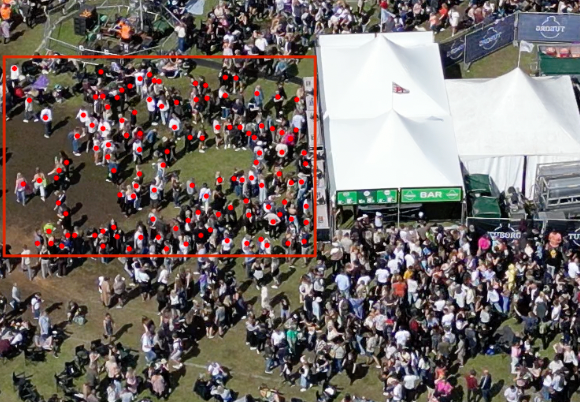
\includegraphics{../images/manual-count1.png}

}

\caption{\label{fig-manual-count1}Small section of bar after concert -
Manual count}

\end{figure}

In the image seen in Figure~\ref{fig-manual-count1}, a section of the
queue to a bar towards the end of a concert. A rough manual count of the
visible people was conducted. This resulted in a count of around 120
people

Now, the same area is highlighted in the frontend to count the people
using the model. This can be seen in Figure~\ref{fig-count-comparison}.

\begin{figure}

{\centering 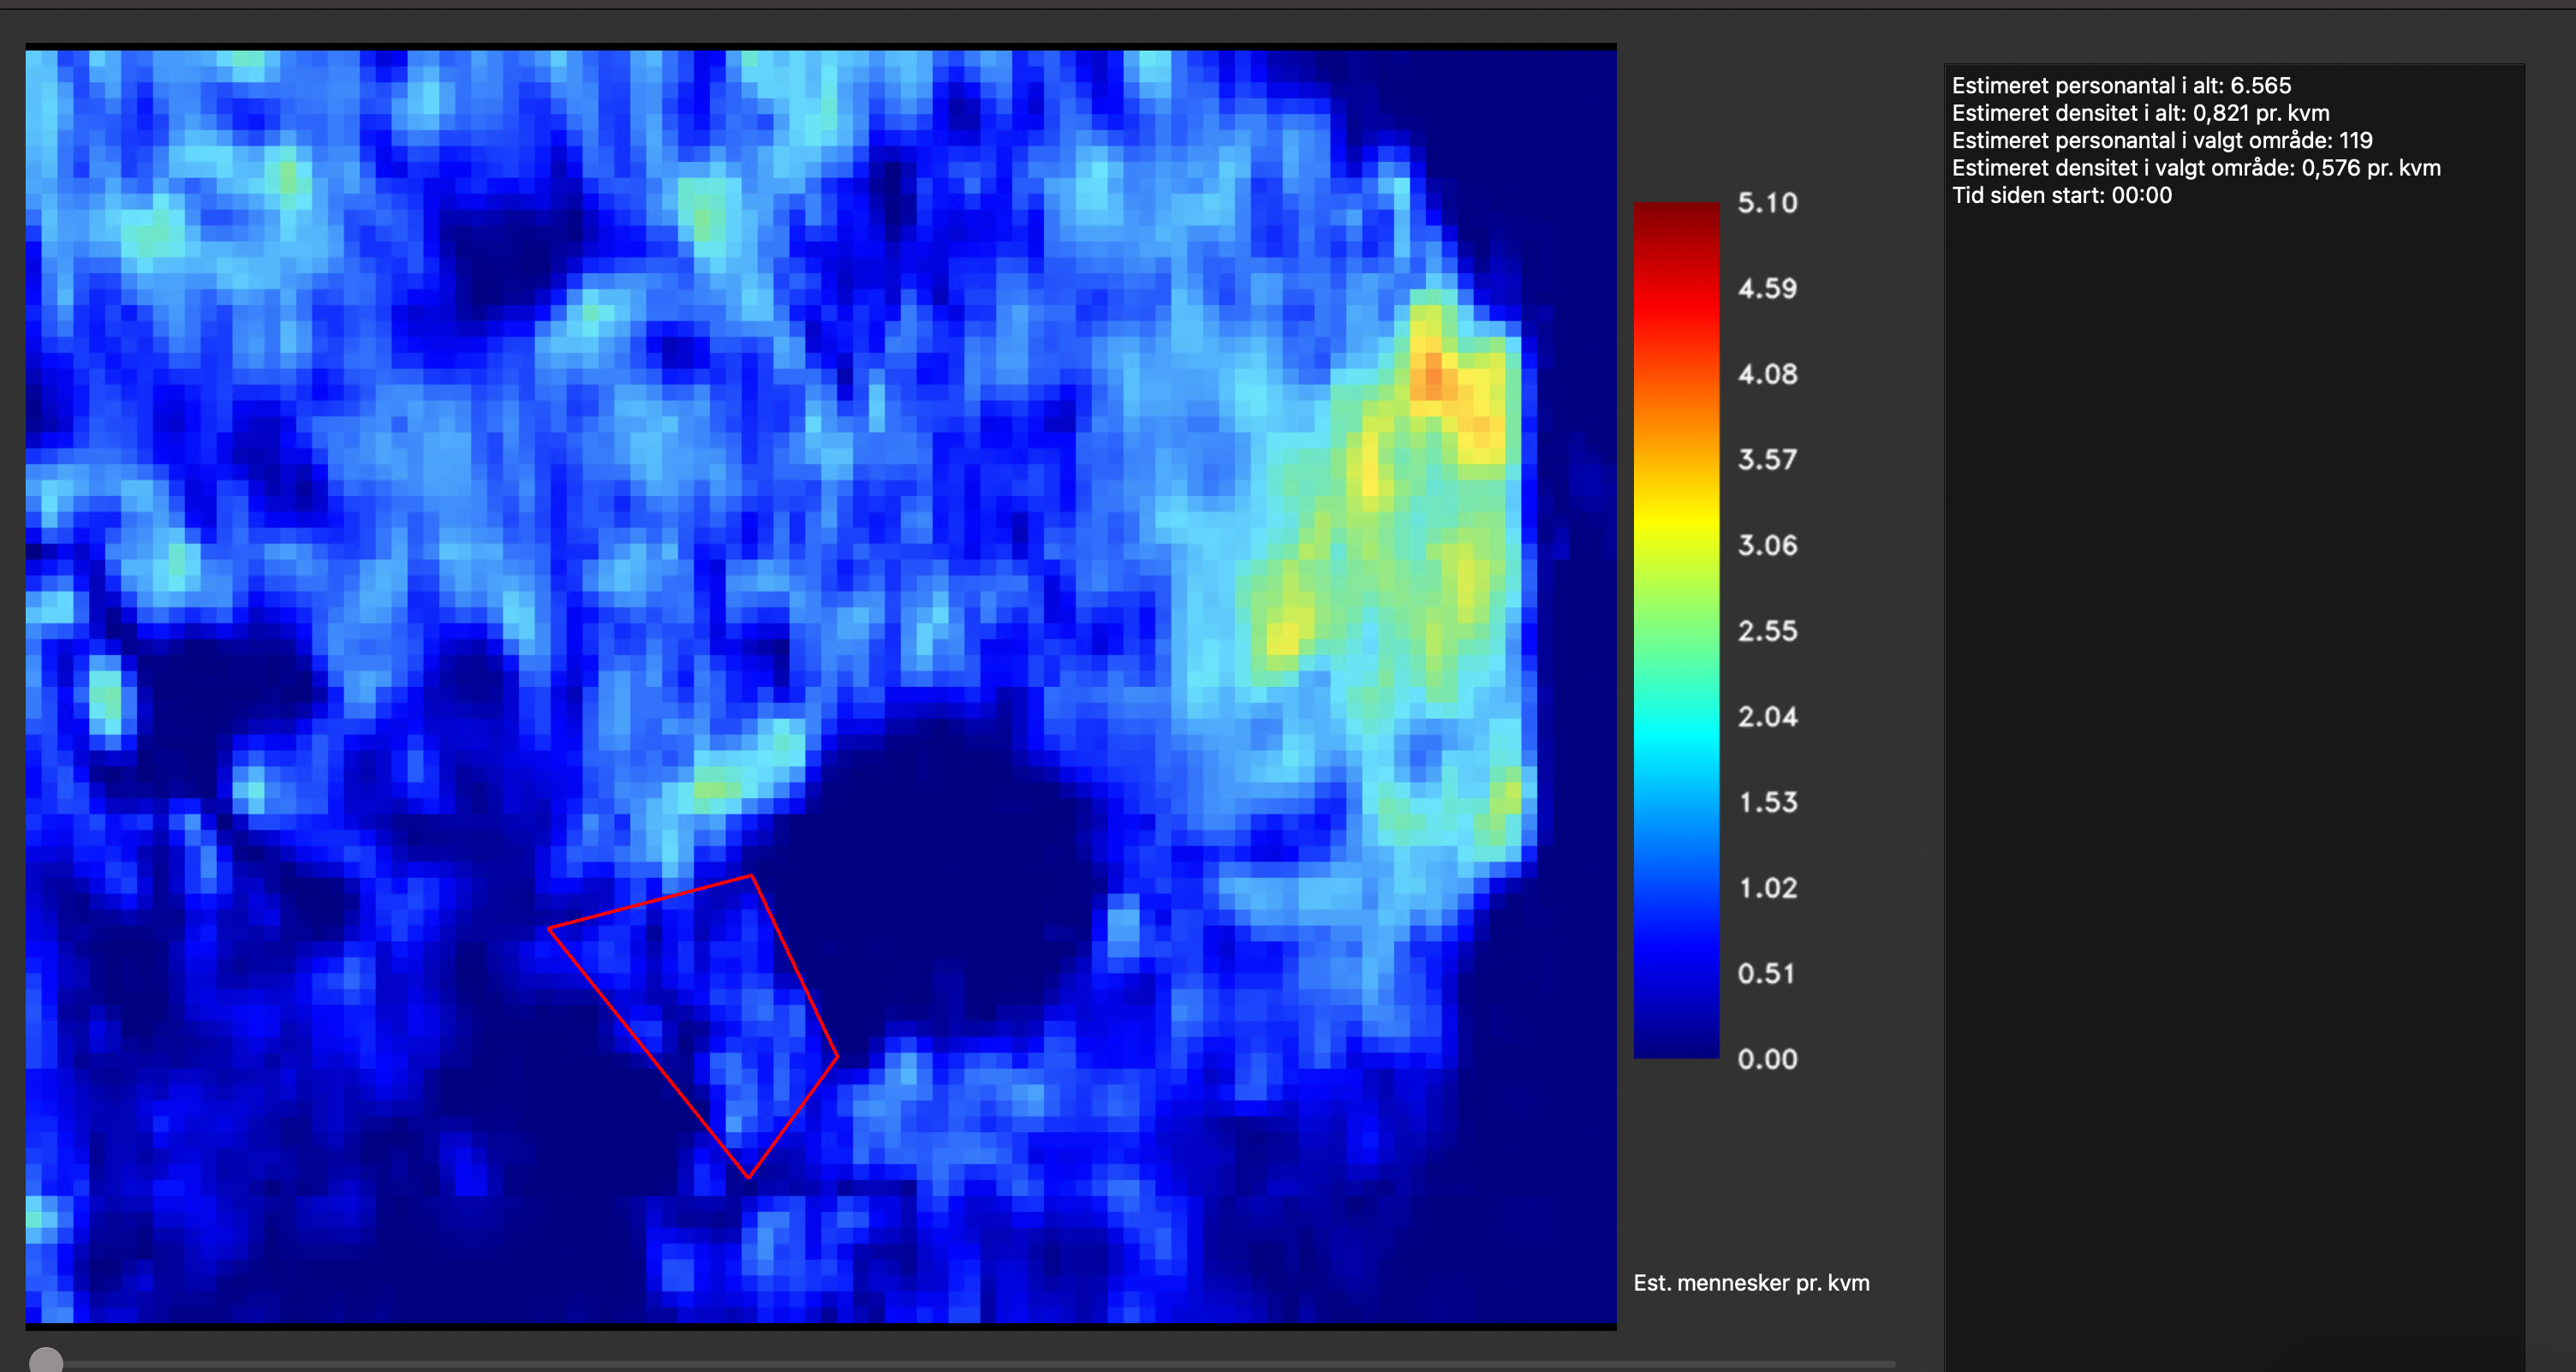
\includegraphics{../images/count-comparison.png}

}

\caption{\label{fig-count-comparison}Small section of bar after concert
- Model count}

\end{figure}

While this test shows that the model is precise in optimal
circumstances, there are of course limitations. The model can only count
as well as a human would be able to. This means that under circumstances
where lighting, stage artifacts (Confetti, fireworks etc.) or bad image
quality is present, the model is unable to count precisely. More on this
in Section~\ref{sec-discussion}

\hypertarget{sec-runtime}{%
\subsection{Runtime and GPU usage}\label{sec-runtime}}

While GPU usage is something already discussed in implementation,
runtime and the optimisation of this are still crucial to test. While we
originally wanted this project to be able to run in real-time, we
quickly realised that this was close to impossible with our current
setup and implementation. When running the model on a video, we
originally ran it on a 3-minute clip with an image every 30 frames being
processed. This resulted in a 180-frame video and a runtime of the
program of around 15 minutes. In the future, if we want to run this
live, additional resources or optimisation is required. Alternatively,
the frame sampling interval could be adjusted to match the speed of the
inference process, which would result in a very low frame rate, but
likely still useful. More about this in Section~\ref{sec-perspective}.

\hypertarget{event-safety-presentation}{%
\subsection{Event Safety presentation}\label{event-safety-presentation}}

Based on the analysis, design and development of the crowd management
system we were invited to present our project to more people from Event
Safety. Research was conducted into how a proper focus group is
structured and managed properly, to give the best possible feedback and
evaluation on the project.

\hypertarget{sec-focusgroup}{%
\subsubsection{Focus group}\label{sec-focusgroup}}

A focus group's purpose is described as: ``As a summative evaluation,
focus groups can be used to assess the acceptance of a new campaign or
gauge customer satisfaction levels''
(\protect\hyperlink{ref-designers_research_manual}{Jenn and Visocky
O'Grady 2017}). This fits the needs and possibilities for this
evaluation. Based on research from this book we arrived at the following
conclusion for our focus group:

\begin{itemize}
\tightlist
\item
  A group of 6-9 people is the preferred group size
\item
  A group of similarly experienced people is needed to encourage a
  proper discussion
\item
  If possible, have more groups with different people
\end{itemize}

For the presentation, a group of 8 employees from Event Safety attended
the presentation with questions and feedback for us along the way. The
employees all had major experience with crowd management and event
planning. Most of them had heard of our project beforehand but had no
further technical insight. The presentation consisted of a short
introduction to the background, context and process, a live
demonstration of the CSMS containing real examples of situations and
concerts they know about, followed by a questionnaire that gives
quantitative and qualitative data on the evaluation.

The focus group session started with an exercise, asking them to
estimate the amount of people in a large crowd section. They were only
given the meta information such as the time of day, place and size of
the area. This was intended to help us validate the idea. Their range
estimates varied from 2.000 to 12.000 in a section with 6.000 crowd
members. This is often the current process when making density and crowd
count estimates, although sometimes helped in real life by other data
such as turnstile counts and tickets sold. This validates the system
because of the large uncertainty in their estimates. Safety guards could
be working against each other's interests if one believes there are
2.000 people in an area, while another believes there are 12.000 people.

\hypertarget{sec-questionnaire}{%
\subsubsection{Focus Group Questionaire}\label{sec-questionnaire}}

Following the focus group, a questionnaire is conducted to gain further
insight. Normally, a questionnaire is used to gather information from a
large group. For our presentation, we still felt a questionnaire was
relevant in order for us to be able to document their answers in a
written format.

The questionnaire was conducted using Mentimeter and consisted of
scales, open-ended questions and rankings. This section will highlight
some of the answers the attendees provided. All the questions and their
results (in Danish) can be found in Section~\ref{sec-appendices}.\\

\textbf{1: To which degree can you see the usefulness in this system for
live events and for post-event evaluations?}\\
In question 1 the participants are asked to verify the need for the
product and the system as a whole. They are asked what they think the
usefulness of the system is as a whole for post-event evaluations (4,6 /
5) and as a live system (4,4 / 5). This verifies that there is a need
for the product and that it has been a correct prioritisation to focus
on a post-event evaluation tool while still having a use case in making
the process live in the future.

\textbf{2: Non-functional system properties}\\

\begin{figure}

{\centering 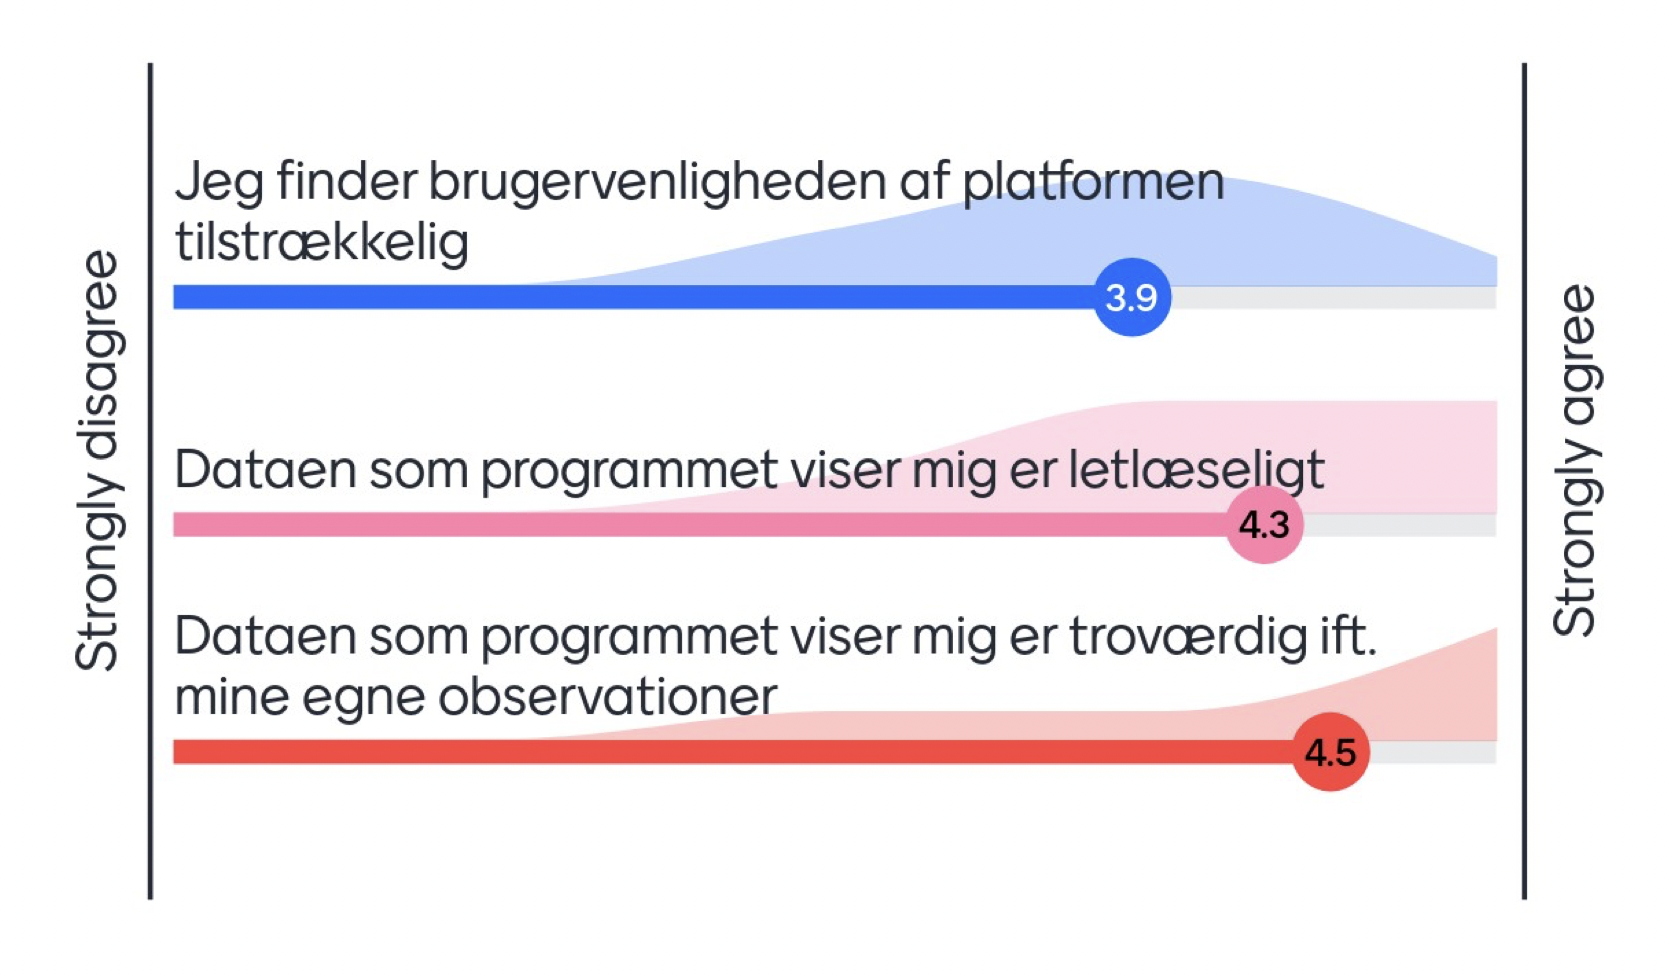
\includegraphics{../images/Evaluation_question2.png}

}

\caption{\label{fig-evaluation_question_2}Questionnaire question 2}

\end{figure}

Question 2 had the attendees evaluate 3 statements on a scale of 1 to 5
and ``strongly disagree'' to ``strongly agree''. 1 being disagree and 5
being agree.

The 3 statements were as follows:

\begin{enumerate}
\def\labelenumi{\arabic{enumi}.}
\item
  I find the usability of the platform adequately simple.
\item
  The data the program visualises is easy to read and understand.
\item
  The data the program provides is credible compared to my own
  observations.
\end{enumerate}

The first statement was evaluated to a score of 3,9, showing that while
the platform in general seems intuitive and fulfills non-functional
requirement 2, there is room for visual improvements.

Statement 2 further validates the implementation of non-functional
requirement \#2 with a score of 4,3.

Statement 3 shows that the professional observations from our attendees
align with the output of our program, showing that functional
requirement 1 is fulfilled.

An attendee also mentioned that the heatmap provided by the program
gives more value than a precise count of individuals in a crowd. This
comment was unfortunately not documented.

\textbf{3: Accuracy and uncertainty of the system}\\

\begin{figure}

{\centering 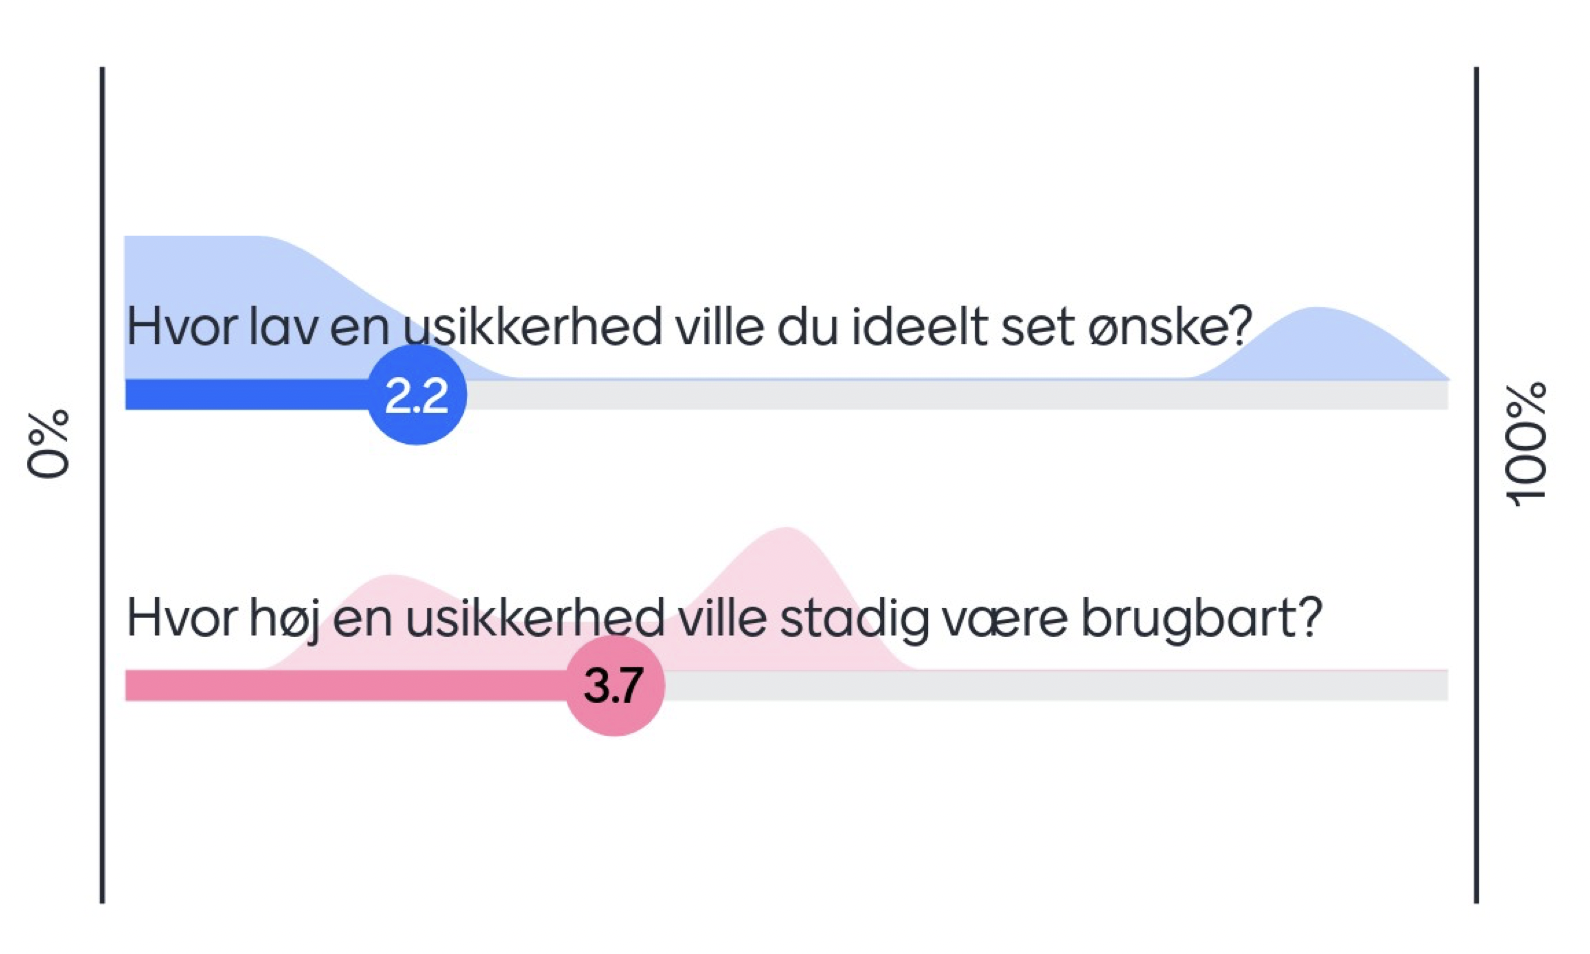
\includegraphics{../images/Evaluation_question3.png}

}

\caption{\label{fig-evaluation_question_3}Questionnaire question 3}

\end{figure}

Question 3 had the attendees evaluate 2 statements from 0 to 100\% based
on their preferred uncertainty of the data provided.

\begin{enumerate}
\def\labelenumi{\arabic{enumi}.}
\item
  What percentage of uncertainty would you prefer?
\item
  How high of an uncertainty would you be willing to accept?
\end{enumerate}

Statement 1 shows a score of 2,2, meaning an uncertainty of around 22\%
would be ideal for the crowd-counting values provided by the program.
This is useful to evaluate functional requirement 1.

Statement 2 shows a score of 3,7, meaning an uncertainty of around 37\%
would still be useful. This further ties into the comment made to
question 2, that the precision of the counts is not as important as the
visualised density maps - though these do rely on each other.

It is also important to note that the required uncertainty percentages
vary depending on the total size of the crowd.

\hypertarget{sec-eval_functional_requirements}{%
\subsection{Evaluation of functional
requirements}\label{sec-eval_functional_requirements}}

Based on the results and evaluation of our presentation for Event Safety
personnel, we can say the following about our functional requirements:

\begin{enumerate}
\def\labelenumi{\arabic{enumi}.}
\tightlist
\item
  The system \textbf{must} be able to count the number of people in the
  crowd with the precision required by the user base
\end{enumerate}

The system can use the model to count crowds of people where a human
would be able to. When lighting conditions or materials from a concert
(bright lights, confetti, fireworks etc.) are present, crowd counting
precision is dramatically reduced. Based on answers in question 3 and
previous conversations with Event Safety, we learned that a higher
precision is not as desirable as a proper heatmap. This meant that focus
was put on perspective warping and generating a proper heatmap of
density in favor of \emph{very} precise crowd counting.

\begin{enumerate}
\def\labelenumi{\arabic{enumi}.}
\setcounter{enumi}{1}
\tightlist
\item
  The system \textbf{must} be able to segment the crowd into virtual
  sections for further processing.
\end{enumerate}

When the processed video is uploaded to our frontend, the user can
select a polygon for further processing. The program provides a count
and density value for the specified area.

\begin{enumerate}
\def\labelenumi{\arabic{enumi}.}
\setcounter{enumi}{2}
\tightlist
\item
  The system \textbf{must} be able to create a heatmap of the crowd
  density.
\end{enumerate}

The system creates a heatmap of the analysed video to visualise crowd
density. The user can select the color scheme of the heatmap themselves
before uploading a video.

\begin{enumerate}
\def\labelenumi{\arabic{enumi}.}
\setcounter{enumi}{3}
\tightlist
\item
  The system \textbf{should} be able to calculate the physical density
  of humans per area unit.
\end{enumerate}

The system can calculate and display the physical density based on the
sum of pixel values in a given area, as each pixel value corresponds to
a certain amount of people. This is dependent on a land survey.

\begin{enumerate}
\def\labelenumi{\arabic{enumi}.}
\setcounter{enumi}{4}
\tightlist
\item
  The system \textbf{should} be able to detect the movement of crowd
  sections.
\end{enumerate}

The system is not directly able to detect the movement of a crowd.
However, the system does create a timelapse of the area in a video which
can be used to manually follow certain crowd movements. According to the
focus group evaluation, it is a desired feature to be able to follow the
flow in and out of a selected area.

\begin{enumerate}
\def\labelenumi{\arabic{enumi}.}
\setcounter{enumi}{5}
\tightlist
\item
  The system \textbf{should} be able to correct for camera distortion,
  warp, and perspective.
\end{enumerate}

The system can correct for perspective by providing ground measurements
and image coordinates to the cv2.warpPerspective() method of the OpenCV
library. The system cannot currently correct for fish eye distortion.

\begin{enumerate}
\def\labelenumi{\arabic{enumi}.}
\setcounter{enumi}{6}
\tightlist
\item
  The system \textbf{should} be able to detect choke points in the crowd
  movements.
\end{enumerate}

The system is not able to detect chokepoints beyond manual observations
of the users.

\begin{enumerate}
\def\labelenumi{\arabic{enumi}.}
\setcounter{enumi}{7}
\tightlist
\item
  The system \textbf{should} be able to generate a summarising report of
  the concert with statistics of (crowd density, crowd count, risk
  factors, choke points, and other) relevant safety indicators after the
  event.
\end{enumerate}

The system is not able to generate a report of every statistic provided
here. The report is based on the current frame of the timelapse and
shows crowd count and crowd density.

\begin{enumerate}
\def\labelenumi{\arabic{enumi}.}
\setcounter{enumi}{8}
\tightlist
\item
  The system \textbf{could} be able to estimate a numerical risk factor
  based on available factors.
\end{enumerate}

The system is not able to estimate a numerical risk factor.

\begin{enumerate}
\def\labelenumi{\arabic{enumi}.}
\setcounter{enumi}{9}
\tightlist
\item
  The system \textbf{could} be able to generate a live, or delayed,
  video overlaid user interface.
\end{enumerate}

The system can generate a delayed video user interface based on the
input. It is not live.

\hypertarget{sec-eval_non_functional_requirements}{%
\subsection{Evaluation of non-functional
requirements}\label{sec-eval_non_functional_requirements}}

Likewise, we can say the following about our non-functional requirements

\begin{enumerate}
\def\labelenumi{\arabic{enumi}.}
\item
  The system \textbf{must} protect the privacy of personal data.\\
  The system only handles sensitive when analysing the surveillance
  footage. The only way the data is ever close to online is when it is
  processed on UCloud. However, as the only online part of the process
  is the usage of UCloud GPUs, the data is never compromised.
\item
  The system \textbf{should} have a user-friendly interface that is easy
  to manage for both technical and non-technical users.\\
  The system has a user-friendly interface that is easy to manage for
  both technical and non-technical users. This is based on the answers
  provided in Section~\ref{sec-focusgroup}. With an average score of
  3,9, there is still room for improvement.
\item
  The system \textbf{should} have adequate documentation/technical
  specifications for technical users.\\
  The backend has a README.md file which instructs technical users on
  how to run the backend as well as system requirements. This can be
  seen in the backend/README.md and in Section~\ref{sec-appendices}.
\item
  The system \textbf{should} have adequate user manuals for
  non-technical users.\\
  The frontend has a user guide with instructions on how to use the
  frontend CSMS and the videos produced by the technical users in the
  backend. This can be seen in Section~\ref{sec-appendices}.
\item
  The system \textbf{could} have high reliability that is not based on
  the visual circumstances and environment (e.g.~sunlight, stage light,
  audience flashlights, and other visual effects) or report confidence
  based on the environment.\\
  See Section~\ref{sec-eval_functional_requirements}
\item
  The system \textbf{could} be scalable to simultaneous interoperability
  between multiple cameras.\\
  The system can provide output from multiple sources of input at the
  same time. While this should also be a functional requirement for it
  to be fully satisfied, the system has been implemented with this in
  mind, making it easily scalable to multiple cameras. The focus group
  evaluation showed that this is one of the most wanted properties of
  the system.
\item
  The system \textbf{could} integrate with existing CCTV software
  systems at venues.\\
  The system is not able to integrate with existing CCTV beyond the
  footage provided to it.
\end{enumerate}

\newpage{}

\hypertarget{sec-operation}{%
\section{Operation}\label{sec-operation}}

This section will describe the plan for operation. Due to the seasonal
nature of festivals, it has not been possible to test the system in
operation at a real festival or concert, nor has it been possible to
collect more or improved data. Thus the ``operation and
maintenance''-phase of the Waterfall model from Sommerville
(\protect\hyperlink{ref-sommerville2011software}{2011}) has not been a
priority in the project. The project's purpose was as a proof of concept
from the beginning. However, the system has been designed with
maintainability in mind

The frontend and backend code bases are maintainable for a few reasons.
The Python code has been written using type hints. Even though typing is
not supported by the Python runtime {``Python Documentation''}
(\protect\hyperlink{ref-PythonDocumentation}{2023}), it is used by IDE's
and linters to enforce good coding practice. The system is also written
using an OOP paradigm which makes it easier to understand due to the
abstraction of implementation. Writing the code in pair programming also
helps maintainability as knowledge is shared and not isolated. When
necessary, this knowledge has been documented in README files.

There are no developers in Event Safety. This means that there have not
been any considerations for development handover or for second part
developers to get involved in the process. For the product to get
applied in their day-to-day work it would take building up a small
catalogue of processed videos of different examples from different
venues. The frontend could be handed over to the users. Users would be
employees and volunteers at Event Safety, Smukfest and Grøn Koncert.
This would provide significant value based on our focus group research.

\newpage{}

\hypertarget{sec-discussion}{%
\section{Discussion}\label{sec-discussion}}

This section will discuss our results including the accuracy of the CSMS
and qualitative user feedback from our partners. It will describe how
this system could affect the crowd safety management flow. It will also
discuss the current system's shortcomings and what can be done in the
future to prevent this. Then it will discuss how this system is an
improvement from the status quo. It will discuss the privacy and ethical
concerns that might be with a system that deals with personal data.
Finally, it will also evaluate the process of developing this system and
on the choice of technologies.

To evaluate the accuracy of the developed system we first look at the
quantitative benchmark of SASNet. Here it was stated that SASNet
performs better or on par with several other state-of-the-art crowd
counting models. On the ShanghaiTech part A specifically, which the
model weights used in the CSMS are trained on, SASNet performs with a
mean average error of 53.59 (\protect\hyperlink{ref-sasnet}{Song et al.
2021}). According to Modolo et al.
(\protect\hyperlink{ref-modolo2021understanding}{2021}), the Shanghai
Tect Part A has an average of 500 people in each image, meaning the
average error percentage is 10.6\% on this dataset. This is the dataset
that most closely matches our spread and density distributions in the
collected data. When doing our testing as described in
Section~\ref{sec-accuracy} we achieve a similar, good accuracy. The
required accuracy according to our user research in
Section~\ref{sec-focusgroup} is that an accuracy of less than 10-20\% is
ideal, but 20-40\% might still be useful. This is well within the bounds
of the accuracy of the CSMS.

However, our accuracy is limited by the important factor that our system
as a whole aims to calculate the actual crowd count of the physical
space and not just the crowd count of the countable crowd members on the
video footage. As an example, we would likely achieve a 0\% error if the
camera was low enough to only count a handful of members, but this is
useless in regards to the overall problem statement of improving the
crowd overview for security guards. It is uncertain how prevalent this
type of uncertainty is in our data, as we do not have this real ground
truth. The limiting factors for achieving this goal are:

\begin{enumerate}
\def\labelenumi{\arabic{enumi}.}
\item
  The cameras must have a high point of view so the maximum amount of
  crowd members are visible.
\item
  The lighting must be good enough to distinguish members of the crowd.
\item
  Stage effects (smoke, confetti) must not cover members of the crowd.
\item
  Video compression artifacts must not be too prominent.
\item
  The camera must be in focus.
\end{enumerate}

While the collected data for these purposes is a good starting point, it
is important to have these factors in mind when collecting data in the
future. Some of these factors are difficult to affect because of other
circumstances. Number 1 in the list above is limited by drone law
regulations or the height of the stage or nearby masts. Number 2 is
difficult during night concerts. It could be possible by installing
night vision or infrared cameras, but it is uncertain how SASNet would
perform with this kind of input data. Number 3 is not possible to affect
directly, but camera angles could affect how stage effects affect the
input data. It might also be useful to sample frames from moments
without many stage effects. Numbers 4 and 5 should be manageable by
using proper camera setups.

Based on the section Section~\ref{sec-eval_functional_requirements} the
CSMS at this point fully satisfies all the ``must have'' functional
requirements and 1 ``should have'' requirement (requirement 4). It also
satisfies most of functional requirements 6 and 8, while functional
requirements 5 and 7 are not directly implemented. The ``could have''
requirements 9 and 10 have not been implemented. In regards to our
evaluation of the non-function requirements in
Section~\ref{sec-eval_non_functional_requirements}, the ``must have''
and ``should have'' requirements are fulfilled. The ``could have''
requirements are partly fulfilled. Particularly the ``could have''
requirement 6 regarding ``interoperability between multiple cameras''
was paid attention during the implementation as this was found to be
important for the company. According to our focus group results in
Section~\ref{sec-focusgroup}, the good feedback, on the trustworthiness
of the output data and the usefulness of the heatmap, validates the
implementation of a large part of the functional and non-functional
requirements. The qualitative feedback from the focus group also
verifies the need for the problem statement and the usefulness of a
system like this in general compared to the status quo, which is manual
estimates of crowd count and densities. According to
Section~\ref{sec-validation-verification} The CSMS is both faster and
more accurate than manual estimates.

The project's collaborators did not have many ethical concerns when
asked. However, it is still our responsibility as the experts, to have
these considerations. That is why we researched the data policy of the
cloud provider UCloud which satisfied the need for data privacy and
responsible use. The ethical considerations were also one of the reasons
why we decided to use the regression-based crowd counting method of
SASnet rather than ``crowd count by detection''. The crowd count based
methods remove the detection of individuals as each output pixel could
be an aggregate of many Gaussian kernels, as described in
Section~\ref{sec-design-crowdcounting}. The extent of discriminatory
biases in the dataset and algorithms such as racial, gender or handicap
has not been tested. Using a crowd count algorithm should be less biased
than the counting by detection algorithm, making it unlikely that it has
a large impact on the final result. However, the choice of crowd
counting method made the implementation of some functional requirements,
in regards to tracking the movement of crowd members, more difficult to
implement which resulted in them not being implemented. A workaround
could be implemented while still using SASNet by looking at delta
changes in densities over multiple time periods, but it is not trivial
to infer the average paths of crowd members (functional requirement 5).

Following these considerations and results, ``crowd count by detection''
and specifically SASnet's way of solving the scale variation has proved
to be a reliable, accurate and fast way of crowd counting, while also
reducing the potential ethical concerns of a system that creates data of
tracked individuals.

The planned timeline of the project was followed and did not prove to be
too tight. The timeline could have been slightly improved by also having
a way of gathering data after having learned the lessons of the
implementation phase, but this was not possible due to the time of year.
Some would perhaps argue that the fact that we were able to follow the
planned timeline is a sign that more work could have been done, but that
was not the case. The prioritisation of the requirements and planning of
the phases resulted in a system that we were able to finish within the
timeframe while still creating a product that was useful for our target
group. The project was completed using a waterfall process rather than a
Scrum process. This was done because the later stages in the design and
implementation phase depend on the knowledge of the earlier stages. This
choice has been a good process for the project since we ended up with a
finished and working proof-of-concept product. A Scrum process could
have resulted in difficulty in meeting deadlines because of the group
size of 2.

\newpage{}

\hypertarget{sec-conclusion}{%
\section{Conclusion}\label{sec-conclusion}}

In conclusion of this project on the Crowd Safety Management System
(CSMS) that uses SASNet for crowd counting and density estimation at
festival events, we look back at what was achieved and the challenges
faced. This is done with regards to the original problem statement from
Section~\ref{sec-problem-statement} that is: ``Can computer vision
software and AI techniques be leveraged to improve crowd overview for
security guards, by receiving video feed from large crowds, and
ultimately improve crowd safety?''

The main success of the project was incorporating a crowd counting
model, specifically SASNet, effectively for density estimation. This
method was very accurate in many crowd situations, which was crucial for
the system's usability at the festivals Grøn and Smukfest. We tested the
system using data from different festivals and under different densities
and circumstances and found success in most common scenarios.

A key part of our work was following GDPR, data privacy and ethical
considerations. This was important because we were dealing with
sensitive video data. We used the crowd count method to keep individual
identities private and instead used aggregate sums of people per square
meter, showing our commitment to ethical data handling and maintaining
the public image of the festivals to festival guests that they and their
sensitive data are safe.

Creating a user-friendly interface was a non-functional requirement. We
wanted the system to be easy to use for both technical and non-technical
users. The interface we developed helped users easily understand complex
data, like heat maps and crowd density figures. It was found from the
focus group session that the heat map is very useful in improving crowd
overview for security guards at post-event evaluations.

We chose to use regression-based methods for crowd counting to avoid
more intrusive methods like tracking individual people. This decision
was important to respect individual privacy and align with ethical
standards in surveillance technology. The technology also proved to be
useful when considering the needed computing power for the alternative.

The project also expectedly faced challenges. Physical environmental
factors like poor lighting and stage effects sometimes affected how
accurately the system worked. These are common issues at festivals and
make maintaining consistent performance difficult.

There were also technical challenges. The system did not fully develop
some features that could be interesting for managing crowds, like
detecting crowd movements and identifying potential choke points.
However, during user testing and discussions, it was not features that
were missing for achieving the overall goal and proving the concept of
the system. Integrating the system with existing CCTV systems was also a
requirement that was not developed because it would not be able to be
tested.

Handling and processing a lot of high-resolution video data was
challenging. We had to balance the need for powerful processing and
storage with the requirement for real-time or near-real-time data
processing. This was a tough task given the amount and type of data we
were dealing with. The delay showed to be around 4-5 seconds for each
frame which is a low enough delay for the use case.

Our focus group evaluation in Section~\ref{sec-focusgroup} shows that
experts on crowd safety find this system extremely useful as a tool in
their work with crowd safety and crowd comfort, successfully proving
this technology and system as a proof-of-concept.

Overall, this project has successfully proved the usefulness of AI and
computer vision techniques for crowd safety management to our company
collaborators. We faced and overcame many challenges and complexities,
creating a system that improves not only crowd safety but also crowd
comfort at festivals. The experiences and knowledge gained from this
project provide a solid base for future developments and improvements in
crowd management and safety systems. These will be summarised in section
Section~\ref{sec-perspective}.

\newpage{}

\hypertarget{sec-perspective}{%
\section{Future Perspectives}\label{sec-perspective}}

There are many opportunities for further development of this project in
collaboration with the company collaborators, under the assumption that
the ethical considerations in Section~\ref{sec-discussion} are kept in
mind.

The current implementation is mostly suitable for post-event
evaluations. This was decided during the design phase, as this would
produce a usable product that was possible to implement. It is, however,
also a possibility to adjust the implementation to allow for a live feed
of the heatmaps, with as little delay as 4-5 seconds on each frame with
the current performance described in Section~\ref{sec-runtime}. Seeing
the heatmaps could open up completely new use cases for the users and
possibly change the workflows of the crowd safety managers and security
camera operators.

The system's use cases are not limited to festivals and concerts. This
can of course be used by any authority or organisation in charge of
large gatherings of people. This could be other users like police,
defence authorities, emergency management agencies, transportation
authorities, sports stadium managers, retail and shopping malls, theme
park managers, for handling events like protests, public national
celebrations (eg. sports celebrations, royal birthdays), sports events,
special days resulting in high-density gatherings like Black Friday, New
Years and Christmas. The only requirement is the ability to collect
usable video input data from a high altitude viewpoint, and a group of
people with the necessary knowledge of crowd safety willing to use the
information provided by the CSMS in a meaningful way to make decisions.

During the design and implementation phase, a multi-camera setup was
briefly investigated as a way of improving the output from venues with
many smaller corridors and no possibility for aerial top-down views
(such as Smukfest). While the collected data was not ideal for this
idea, the current implementation is set up to allow for this, by
defining multiple cameras and their physical bounds.

It could be an interesting perspective to incorporate more
cyber-physical or IoT aspects into this system. Currently, the system
consists of a sensor system with video as input that helps crowd safety
managers in their decision-making. The system could implement an
automated control system for adjusting density imbalances by controlling
entrance flow, affecting human behavior by pushing information through
an app, stage LED screens or public address systems. The sensor system
could also be improved by incorporating more data sources into the
algorithms and predict the crowd behavior, so decisions could be made in
due time. This could be done by implementing an IoT system with a
network of sensor devices such as data from bar sales, turnstiles, crowd
profiles, data from cellphones, etc. and integrating the data into an AI
prediction algorithm.

During our discussions with the drone company PhaseOne, they
demonstrated some interesting technologies regarding drone and camera
technology where this system could be applied. The company provides
software and hardware for extremely high-resolution imagery on drones.
Using this technology it could be possible to cover a very large
geographical area using only one or few drones from a high altitude,
making it possible to cover multiple or spread out gatherings at once
while requiring almost no setup time. Their technology can also allow
for approximate orthographic projections, reducing or completely
removing the need for perspective warp. This technology could be very
useful for open-air festivals with many stages at once, protests and
urban gatherings that are often spread out and high density.

Another interesting idea for further development of this project would
be to advance the project from crowd counting to crowd localisation. As
described in Section~\ref{sec-softa}, crowd localisation is a more
advanced, proposed form of crowd counting. Advancing to an
implementation of this would allow us to further increase the usability
of the program by implementing accurate flow estimation and a more
precise count. This would also open up the possibility of tracking
individual groups of people if users wanted to keep an eye on a certain
section of the crowd. However, going in this direction would likely also
require higher information security, as you would now be tracking the
movement of parts of the crowd.

\newpage{}

\hypertarget{references}{%
\section*{References}\label{references}}
\addcontentsline{toc}{section}{References}

\hypertarget{refs}{}
\begin{CSLReferences}{1}{0}
\leavevmode\vadjust pre{\hypertarget{ref-chan2008}{}}%
Chan, Antoni, John Liang, and Nuno Vasconcelos. 2008. {``Privacy
Preserving Crowd Monitoring: Counting People Without People Models or
Tracking.''} In \emph{Computer Vision and Pattern Recognition}.
\url{https://doi.org/10.1109/CVPR.2008.4587569}.

\leavevmode\vadjust pre{\hypertarget{ref-pytorch}{}}%
Contributors, PyTorch. 2023. \emph{PyTorch Documentation}.
\url{https://pytorch.org/docs/stable/index.html}.

\leavevmode\vadjust pre{\hypertarget{ref-dahl2023crowd}{}}%
Dahl, Sofie. 2023. {``Crowd Management.''} EventSafety.

\leavevmode\vadjust pre{\hypertarget{ref-FELICIANI2023106174}{}}%
Feliciani, Claudio, Alessandro Corbetta, Milad Haghani, and Katsuhiro
Nishinari. 2023. {``Trends in Crowd Accidents Based on an Analysis of
Press Reports.''} \emph{Safety Science} 164: 106174.
https://doi.org/\url{https://doi.org/10.1016/j.ssci.2023.106174}.

\leavevmode\vadjust pre{\hypertarget{ref-fruin1971pedestrian}{}}%
Fruin, John J. 1971. {``Pedestrian Planning and Design.''}

\leavevmode\vadjust pre{\hypertarget{ref-DBLP:journalsux2fcorrux2fabs-2108-00584}{}}%
Gao, Junyu, Maoguo Gong, and Xuelong Li. 2021. {``Congested Crowd
Instance Localization with Dilated Convolutional Swin Transformer.''}
\emph{CoRR} abs/2108.00584. \url{https://arxiv.org/abs/2108.00584}.

\leavevmode\vadjust pre{\hypertarget{ref-gjy3035_awesome_crowd_counting}{}}%
Gong, Jia-Yu. 2023. {``Awesome-Crowd-Counting.''}
\url{https://github.com/gjy3035/Awesome-Crowd-Counting}.

\leavevmode\vadjust pre{\hypertarget{ref-iso27001}{}}%
International Organization for Standardization. 2013. {``{ISO/IEC
27001:2013 - Information security management systems}.''} 2013.
\url{https://www.iso.org/standard/27001}.

\leavevmode\vadjust pre{\hypertarget{ref-designers_research_manual}{}}%
Jenn, and Ken Visocky O'Grady. 2017. \emph{A Designer's Research Manual:
Second Edition, Updated + Expanded}. Second. Rockport Publishers.

\leavevmode\vadjust pre{\hypertarget{ref-NIPS2010_fe73f687}{}}%
Lempitsky, Victor, and Andrew Zisserman. 2010. {``Learning to Count
Objects in Images.''} In \emph{Advances in Neural Information Processing
Systems}, edited by J. Lafferty, C. Williams, J. Shawe-Taylor, R. Zemel,
and A. Culotta. Vol. 23. Curran Associates, Inc.
\url{https://proceedings.neurips.cc/paper_files/paper/2010/file/fe73f687e5bc5280214e0486b273a5f9-Paper.pdf}.

\leavevmode\vadjust pre{\hypertarget{ref-li2021approaches}{}}%
Li, Bo, Hongbo Huang, Ang Zhang, Peiwen Liu, and Cheng Liu. 2021.
{``Approaches on Crowd Counting and Density Estimation: A Review.''}
\emph{Pattern Analysis and Applications} 24: 853--74.

\leavevmode\vadjust pre{\hypertarget{ref-ma2023sam}{}}%
Ma, Zhiheng, Xiaopeng Hong, and Qinnan Shangguan. 2023. {``Can SAM Count
Anything? An Empirical Study on SAM Counting.''}
\url{https://arxiv.org/abs/2304.10817}.

\leavevmode\vadjust pre{\hypertarget{ref-modolo2021understanding}{}}%
Modolo, Davide, Bing Shuai, Rahul Rama Varior, and Joseph Tighe. 2021.
{``Understanding the Impact of Mistakes on Background Regions in Crowd
Counting.''} In \emph{Proceedings of the IEEE/CVF Winter Conference on
Applications of Computer Vision}, 1650--59.

\leavevmode\vadjust pre{\hypertarget{ref-DBLP:journalsux2fcorrux2fOSheaN15}{}}%
O'Shea, Keiron, and Ryan Nash. 2015. {``An Introduction to Convolutional
Neural Networks.''} \emph{CoRR} abs/1511.08458.
\url{http://arxiv.org/abs/1511.08458}.

\leavevmode\vadjust pre{\hypertarget{ref-PythonDocumentation}{}}%
{``Python Documentation.''} 2023. \url{https://docs.python.org/3/}.

\leavevmode\vadjust pre{\hypertarget{ref-inproceedings}{}}%
Raineri, Aldo. 2004. {``The Causes and Prevention of Serious Crowd
Injury and Fatalities at Outdoor Music Festivals.''} In.
\url{https://doi.org/10.13140/2.1.3036.0005}.

\leavevmode\vadjust pre{\hypertarget{ref-UCloud_Security}{}}%
SDU Cloud. 2020. {``{Introduction to Cloud Security}.''} 2020.
\url{https://docs.cloud.sdu.dk/intro/security.html}.

\leavevmode\vadjust pre{\hypertarget{ref-simonyan2014very}{}}%
Simonyan, Karen, and Andrew Zisserman. 2014. {``Very Deep Convolutional
Networks for Large-Scale Image Recognition.''} \emph{arXiv Preprint
arXiv:1409.1556}.

\leavevmode\vadjust pre{\hypertarget{ref-sommerville2011software}{}}%
Sommerville, I. 2011. \emph{Software Engineering}. International
Computer Science Series. Pearson.
\url{https://books.google.es/books?id=l0egcQAACAAJ}.

\leavevmode\vadjust pre{\hypertarget{ref-sasnet}{}}%
Song, Qingyu, Changan Wang, Yabiao Wang, Ying Tai, Chengjie Wang, Jilin
Li, Jian Wu, and Jiayi Ma. 2021. {``To Choose or to Fuse? Scale
Selection for Crowd Counting.''} \emph{The Thirty-Fifth AAAI Conference
on Artificial Intelligence (AAAI-21)}.

\leavevmode\vadjust pre{\hypertarget{ref-Still2014CrowdScience}{}}%
Still, G. Keith. 2014. \emph{Introduction to Crowd Science}. CRC Press.

\leavevmode\vadjust pre{\hypertarget{ref-cv2-warpperspective}{}}%
The AI Learner. n.d. {``{OpenCV cv2.warpPerspective() Function}.''}
\url{https://theailearner.com/tag/cv2-warpperspective/}.

\leavevmode\vadjust pre{\hypertarget{ref-Zhang_2016_CVPR}{}}%
Zhang, Yingying, Desen Zhou, Siqin Chen, Shenghua Gao, and Yi Ma. 2016.
{``Single-Image Crowd Counting via Multi-Column Convolutional Neural
Network.''} In \emph{Proceedings of the IEEE Conference on Computer
Vision and Pattern Recognition (CVPR)}.

\end{CSLReferences}

\newpage{}

\hypertarget{sec-appendices}{%
\section{Appendix}\label{sec-appendices}}

\hypertarget{technical-specifications-for-camera}{%
\subsection*{Technical specifications for
camera}\label{technical-specifications-for-camera}}
\addcontentsline{toc}{subsection}{Technical specifications for camera}

\begin{figure}

{\centering 
\includegraphics{../appendices/teknisk-specifikation.png}

}

\caption{\label{fig-camera-specs}Technical specification document for
cameras}

\end{figure}

\newpage{}

\hypertarget{full-class-diagram-for-frontend}{%
\subsection*{Full class diagram for
frontend}\label{full-class-diagram-for-frontend}}
\addcontentsline{toc}{subsection}{Full class diagram for frontend}

\begin{figure}

{\centering 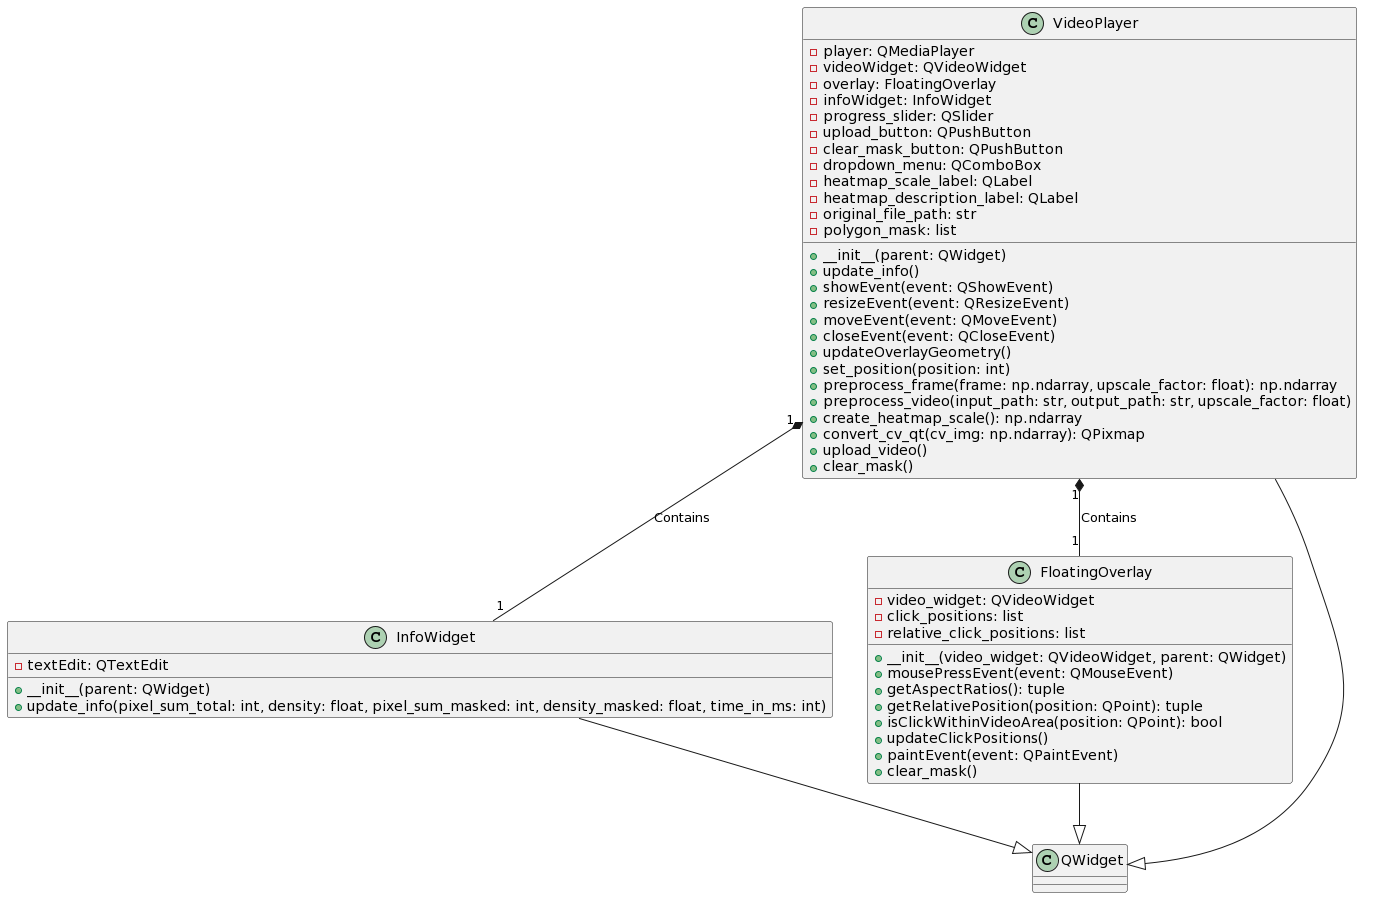
\includegraphics[width=\textwidth,height=0.9\textheight]{../images/class-diagram-frontend-full.png}

}

\caption{\label{fig-frontend-class-diagram-full}Class diagram for
frontend}

\end{figure}

\newpage{}

\hypertarget{timeline}{%
\subsection*{Timeline}\label{timeline}}
\addcontentsline{toc}{subsection}{Timeline}

\begin{longtable}[]{@{}
  >{\raggedright\arraybackslash}p{(\columnwidth - 2\tabcolsep) * \real{0.5000}}
  >{\raggedright\arraybackslash}p{(\columnwidth - 2\tabcolsep) * \real{0.5000}}@{}}
\toprule\noalign{}
\begin{minipage}[b]{\linewidth}\raggedright
\textbf{Date}
\end{minipage} & \begin{minipage}[b]{\linewidth}\raggedright
\textbf{Activity}
\end{minipage} \\
\midrule\noalign{}
\endhead
\bottomrule\noalign{}
\endlastfoot
July-August & Gathering data at attended festivals in collaboration with
Event Safety \\
& \\
August & Drafting the project description \\
& \\
31-08-2023 & Delivering the project description \\
& \\
09-09-2023 & Final discussion with Event Safety regarding the proposed
solutions, requirements and the project going forward \\
September & In-depth analysis of use cases (with Event Safety) In-depth
analysis of required technologies and methods used in academic
literature. Design of the system \\
& \\
25-09-2023 & Progress update with Event Safety regarding the design of
the system \\
& \\
October & Implementation of proof of concept system (primarily
backend) \\
& \\
26-10-2023 & Progress update with Event Safety and small-scale user
testing \\
& \\
31-10-2023 & Attending Crowd Safety Course hosted by Event Safety in
Copenhagen \\
& \\
November & Implementation of proof of concept system \\
& \\
December & Final implementation of the system Documentation of the
system User testing and evaluation \\
\end{longtable}

\newpage{}

\hypertarget{mentimeter-presentation-result}{%
\subsection*{Mentimeter presentation
result}\label{mentimeter-presentation-result}}
\addcontentsline{toc}{subsection}{Mentimeter presentation result}

\begin{figure}

{\centering 
\includegraphics{../appendices/MentimeterPresentation.pdf}

}

\caption{\label{fig-presentation-results}Mentimeter presentation result}

\end{figure}

\newpage{}

\hypertarget{backend-initialisation-script}{%
\subsection*{Backend initialisation
script}\label{backend-initialisation-script}}
\addcontentsline{toc}{subsection}{Backend initialisation script}

\begin{Shaded}
\begin{Highlighting}[]

\CommentTok{\#!/bin/bash}

\FunctionTok{git}\NormalTok{ submodule init}
\FunctionTok{git}\NormalTok{ submodule update}

\FunctionTok{sudo}\NormalTok{ add{-}apt{-}repository }\AttributeTok{{-}y}\NormalTok{ ppa:deadsnakes/ppa   }
\FunctionTok{sudo}\NormalTok{ apt{-}get update}
\FunctionTok{sudo}\NormalTok{ apt{-}get install }\AttributeTok{{-}y}\NormalTok{ libgl1{-}mesa{-}glx}

\CommentTok{\# Install Python 3.7 and the distutils package which is required for pip installation}
\FunctionTok{sudo}\NormalTok{ apt{-}get install }\AttributeTok{{-}y}\NormalTok{ python3.7 python3.7{-}distutils}

\CommentTok{\# Set Python3.7 as the default python3 installation}
\FunctionTok{sudo}\NormalTok{ update{-}alternatives }\AttributeTok{{-}{-}install}\NormalTok{ /usr/bin/python3 python3 /usr/bin/python3.7 1}
\FunctionTok{sudo}\NormalTok{ update{-}alternatives }\AttributeTok{{-}{-}config}\NormalTok{ python3}

\CommentTok{\# Install pip for Python3}
\FunctionTok{sudo}\NormalTok{ apt{-}get install }\AttributeTok{{-}y}\NormalTok{ python3{-}pip}

\CommentTok{\# Upgrade pip to the latest version}
\ExtensionTok{python3} \AttributeTok{{-}m}\NormalTok{ pip install }\AttributeTok{{-}{-}upgrade}\NormalTok{ pip}

\CommentTok{\# Install packages from the requirements file}
\ExtensionTok{pip}\NormalTok{ install }\AttributeTok{{-}r}\NormalTok{ CrowdCounting{-}SASNet/requirements.txt}
\ExtensionTok{pip}\NormalTok{ install }\AttributeTok{{-}r}\NormalTok{ requirements.txt}
\end{Highlighting}
\end{Shaded}

\hypertarget{crowd-counting-documentation-technical-users}{%
\subsection*{Crowd Counting Documentation (technical
users)}\label{crowd-counting-documentation-technical-users}}
\addcontentsline{toc}{subsection}{Crowd Counting Documentation
(technical users)}

\hypertarget{system-requirements}{%
\subsubsection{System requirements}\label{system-requirements}}

\begin{itemize}
\item
  Debian-based Unix system like Ubuntu.
\item
  Able to execute Bash scripts with root access.
\item
  Git installed.
\item
  Internet access.
\end{itemize}

\hypertarget{step-by-step-guide}{%
\subsubsection{Step-by-step guide}\label{step-by-step-guide}}

\begin{enumerate}
\def\labelenumi{\arabic{enumi}.}
\item
  Clone the repository at \url{https://github.com/anirv20/crowd-safety}.
\item
  Run the init.sh using \texttt{bash\ backend/init.sh}.
\item
  Download the SHHA.pth model weights from
  \href{https://drive.google.com/drive/folders/1uTkJLQOn-jQg81yNAluBpGpIJ-XaZaGI}{SASNet}.
\item
  In main.py: Configure the path to the SHHA.pth model weights.
  (MODEL\_PATH)
\item
  In main.py: Configure the output directory. (OUTPUT\_DIR)
\item
  In main.py: Configure the frame sampling interval. (FRAME\_INTERVAL)
\item
  In main.py: If the intended use is with the frontend: Set
  UPSAMPLING\_FACTOR to 1 and COLOR\_MAP to None.
\item
  In main.py: Define the corners of the cropped area on the video in (x,
  y) pairs in local\_coordinates for each Camera instance.
\item
  In main.py: Define the global coordinates based on the land survey for
  each Camera instance.
\item
  In main.py: Define the path to the camera video for each Camera
  instance.
\item
  In main.py: Add the Camera instance to the same or different Camera
  collections.
\item
  Run main.py and download the output video from the specified
  OUTPUT\_DIR. This can now be uploaded to the frontend if step 7 was
  followed.
\end{enumerate}

\hypertarget{frontend-guide-non-technical-users}{%
\subsection*{Frontend Guide (Non-technical
users)}\label{frontend-guide-non-technical-users}}
\addcontentsline{toc}{subsection}{Frontend Guide (Non-technical users)}

Below is a user guide for the frontend and its functions\\

\begin{figure}

{\centering 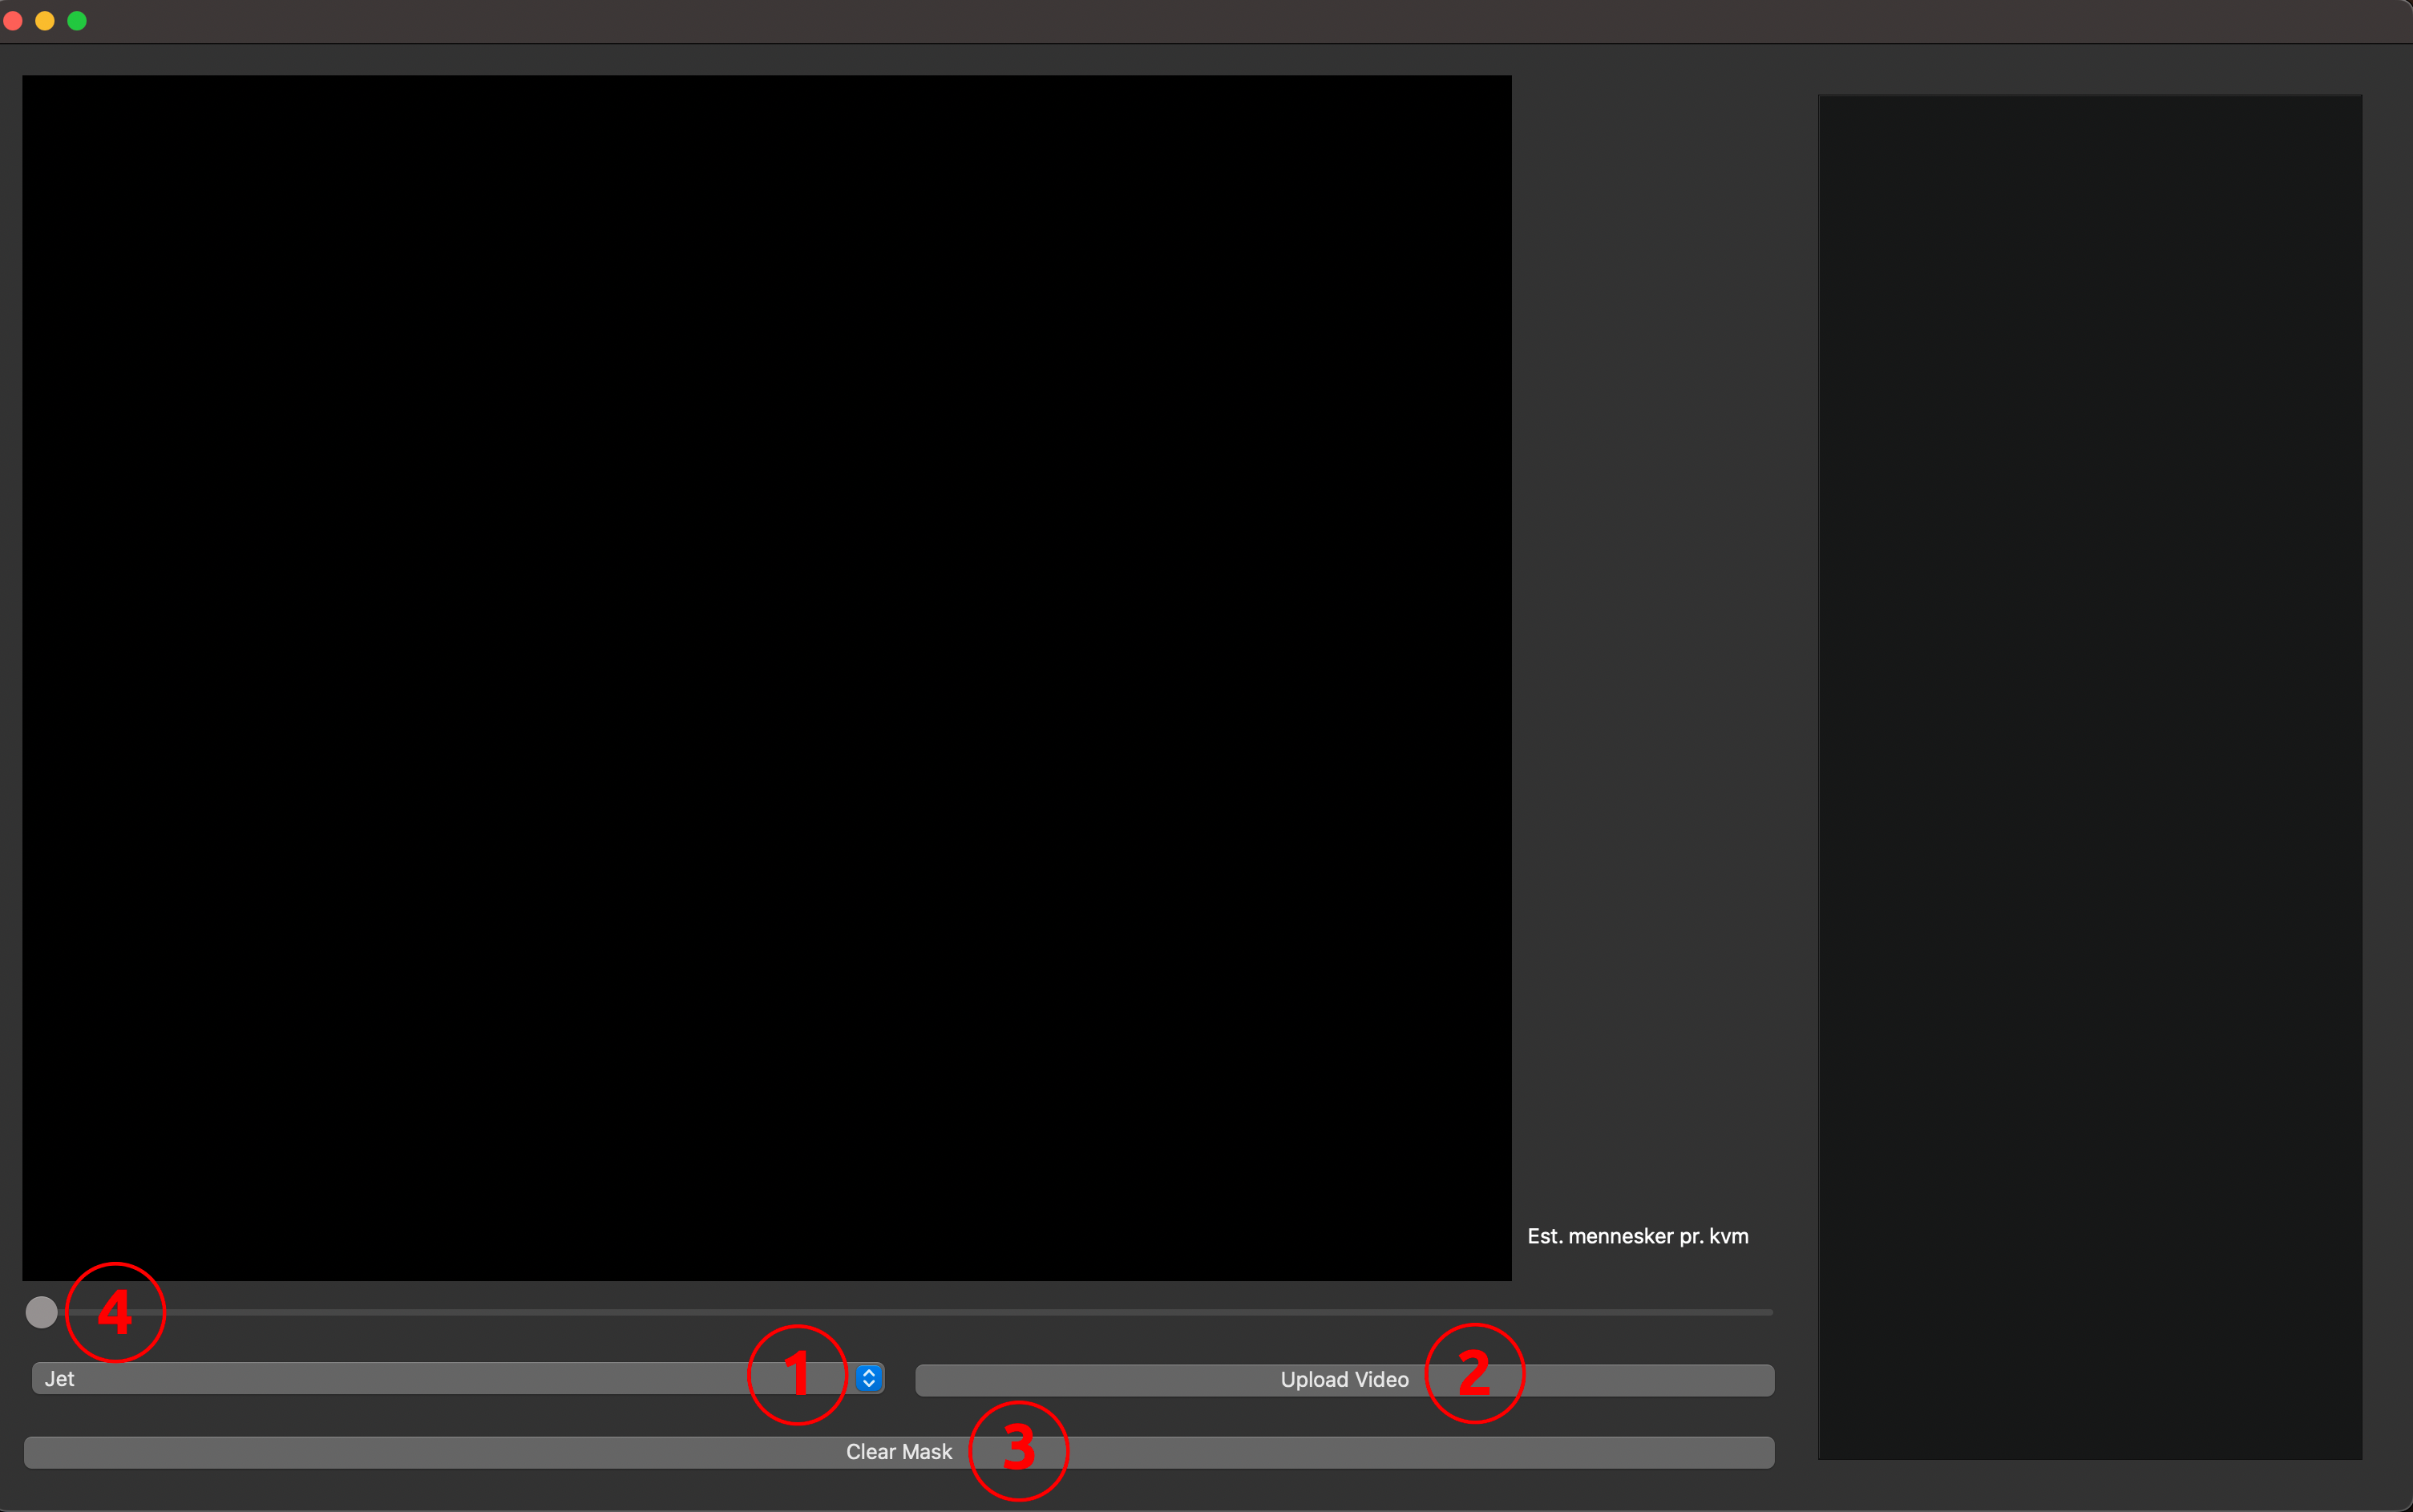
\includegraphics{../appendices/Frontend.png}

}

\caption{\label{fig-frontend}Frontend user guide}

\end{figure}

\begin{enumerate}
\def\labelenumi{\arabic{enumi}.}
\item
  Colorspace for the heatmap. This menu allows the user to select a
  specific color space for the heatmap. The colorspace ``JET'' is
  selected by default
\item
  The upload video button allows the user to upload a video that has
  been processed by the backend
\item
  When a video has been uploaded, the user can use their mouse to select
  a series of points to define an area for specific analysis - See
  Figure~\ref{fig-count-comparison}. This button removes the polygon and
  allows the user to mark a new one.
\item
  When a video is uploaded, the user can use the progress bar to move
  forward or backward in the video.
\end{enumerate}



\end{document}
